% Created with jtex v.1.0.20
\documentclass[a4paper,11pt,oneside]{book}
\usepackage[top=2cm, bottom=2cm, left=2cm, right=2cm]{geometry}
\usepackage[T1]{fontenc}
\usepackage[utf8]{inputenc}
\usepackage{lmodern}
\usepackage{graphicx}
\usepackage{caption}
\usepackage{natbib}
\usepackage{xcolor}
\usepackage{changepage}
\usepackage{framed}
\usepackage{hyperref}
\usepackage{amssymb}
\bibliographystyle{abbrvnat}

% Make list items more compact
\usepackage{enumitem}
\setlist[itemize]{noitemsep, topsep=0pt}

%%%%%%%%%%%%%%%%%%%%%%%%%%%%%%%%%%%%%%%%%%%%%%%%%%
%%%%%%%%%%%%%%%%%%%%  imports  %%%%%%%%%%%%%%%%%%%
\usepackage{booktabs}
\usepackage{url}
%%%%%%%%%%%%%%%%%%%%%%%%%%%%%%%%%%%%%%%%%%%%%%%%%%


\hypersetup{
  colorlinks,
  linkcolor={black},
  citecolor={black},
  urlcolor={black}
}

% Style quotes
\definecolor{darkblue}{rgb}{0.0, 0.0, 0.55}
\definecolor{quoteshade}{rgb}{0.95, 0.95, 1}
\renewenvironment{quote}{%
  \def\FrameCommand{%
    \hspace{1pt}%
    {\color{darkblue}\vrule width 2pt}%
    {\color{quoteshade}\vrule width 4pt}%
    \colorbox{quoteshade}%
  }%
  \MakeFramed {\advance\hsize-\width \FrameRestore}%
  \noindent\hspace{-8pt}% disable indenting first paragraph
  \begin{adjustwidth}{0pt}{0pt}% adjust as needed
  \vspace{2pt}\vspace{2pt}%
}
{%
  \vspace{2pt}\end{adjustwidth}\endMakeFramed%
}

\title{\Huge \textbf{OpenScienceLab Documentation}}
\author{\textsc{The ASF Services Team}}

\begin{document}
\sloppy

\frontmatter
\maketitle

\tableofcontents
% \listoffigures
% \listoftables

\mainmatter

% \include{preface.tex}
% \include{acknowledgements.tex}

\section{Troubleshooting}

\subsection{Troubleshooting Guide}

\newline
\begin{itemize}
\item Why~don’t~any~labs~appear~on~the~OpenScienceLab~home~page?
\item Why~did~the~kernel~die~while~running~a~notebook?
\item I~successfully~ran~a~notebook~earlier~on~the~same~data~but~now~it~is~killing~the~kernel.
\item I~receive~a~Kernel~not~found~message~when~I~open~a~notebook.
\item My~notebook~won’t~open,~opens~slowly,~or~won’t~save.
\item I~am~receiving~a~No~space~left~on~device~error.
\item My~server~won’t~start~and~I~cannot~access~OpenSARlab.
\item The~edits~I~made~to~an~ASF~notebook~have~disappeared~since~the~last~time~I~used~OpenSARlab.
\item One~of~my~notebooks~looks~like~it~has~a~mix~of~code~from~various~versions~of~the~notebook.
\item I~am~having~trouble~setting~up~a~web~server~and~developing~my~web~app~in~OpenSARlab.
\item A~notebook~won’t~load.~A~new~browser~tab~opens~and~shows~the~JupyterHub~header,~but~no~notebook~appears.
\item My~issue~is~not~on~this~list
\end{itemize}

\subsubsection{Why don't any labs appear on the OpenScienceLab home page?}\label{Why-dont-any-labs-appear-on-the-OpenScienceLab-home-page}

You most likely have not yet configured Multi-Factor Authentication (MFA). While
any user can log in without MFA, until a user has configured their MFA device,
they will be unable to access any OpenScienceLab resources.

See \href{/mfa}{Configuring Multi-Factor Authentication} for more information and
a detailed walkthrough.

\subsubsection{Why did the kernel die while running a notebook?}\label{Why-did-the-kernel-die-while-running-a-notebook}

\begin{figure}[!htbp]
\centering
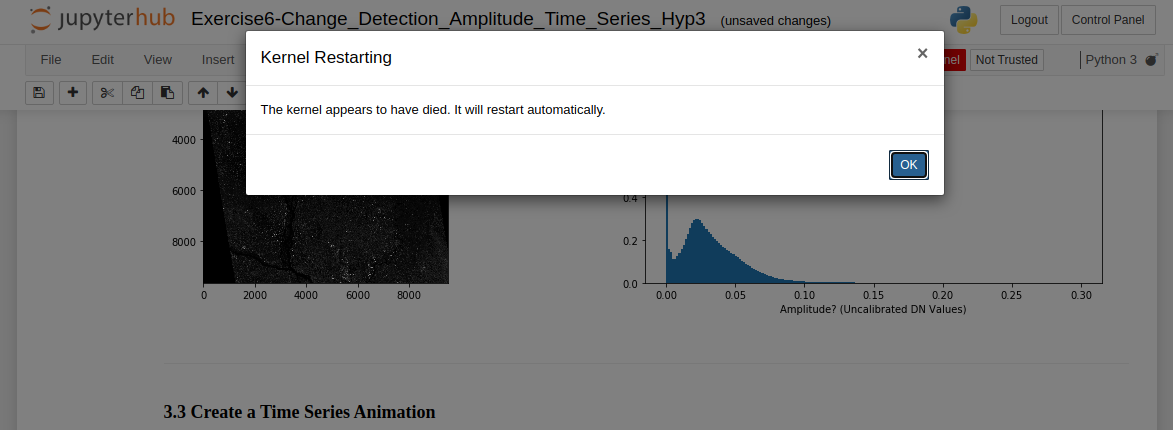
\includegraphics[width=0.7\linewidth]{files/kernel_death-d28efc694e1f525cac874ac5cff0e697.png}
\caption*{The message that appears when a notebook kernel dies}
\end{figure}

\begin{itemize}
\item The kernel will die if you run out of available memory to complete a running process. This occurs frequently when running a time-series or change detection algorithm on data stack that is either too deep or covers too large of an area-of-interest (AOI) for OpenSARLab to handle.


\item Try running the notebook on some combination of a shallower data stack and/or a smaller AOI. This may take some experimentation because memory is shared among users, \textit{i.e.} amount of available memory fluctuates.


\item To work with a deep stack covering an extensive AOI, you may need to tile up your data for the analysis and mosaic them later.
\end{itemize}

\textit{Summary:} If you are running a resource hungry program, your kernel might die. Try subsetting your data, processing it in batches, and mosaicing your results.


\bigskip
\centerline{\rule{13cm}{0.4pt}}
\bigskip

\subsubsection{I successfully ran a notebook earlier on the same data but now it is killing the kernel.}\label{I-successfully-ran-a-notebook-earlier-on-the-same-data-but-now-it-is-killing-the-kernel}

\begin{itemize}
\item OpenSARLab EC2 instances are shared among 1{\textasciitilde}3 users. The memory available to each user depends on overall activity on the EC2. It is likely that there was enough memory available for your process before, but not enough memory during later attempt(s). More details on the OpenSARLab user environment can be found \href{OpenSARLab\_environment.md}{here}.
\end{itemize}


\bigskip
\centerline{\rule{13cm}{0.4pt}}
\bigskip

\subsubsection{I receive a \texttt{Kernel not found} message when I open a notebook.}\label{I-receive-a-Kernel-not-found-message-when-I-open-a-notebook}

\begin{figure}[!htbp]
\centering
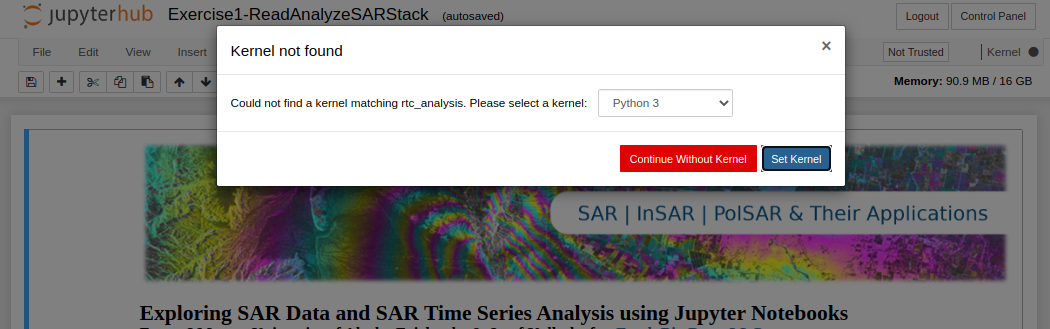
\includegraphics[width=0.7\linewidth]{files/kernel_not_found-b803e941d26eecaaafd4dc583a6ba310.png}
\caption*{The message that appears when an expected notebook kernel cannot be found}
\end{figure}

\begin{itemize}
\item You either have:

\begin{itemize}
\item Not created the required conda environment yet
\item A mix-up between the environment name and prefix
\end{itemize}


\item If you think you already installed the environment, select it from the pull-down menu that appears and click the \texttt{Set Kernel} button.


\item If you have not created the environment yet:

\begin{itemize}
\item In OpenSARLab, you can find a selection of environments and a notebook to build them here: \href{https://opensciencelab.asf.alaska.edu/lab/smce-prod-opensarlab/hub/user-redirect/lab/tree/conda\_environments/Create\_OSL\_Conda\_Environments.ipynb}{\texttt{/home/jovyan/conda\_environments/Create\_OSL\_Conda\_Environments.ipynb}}
\item If you are working in an ASF-supplied Jupyter Book, it should include a notebook to build the required environment/s
\end{itemize}
\end{itemize}


\bigskip
\centerline{\rule{13cm}{0.4pt}}
\bigskip

\subsubsection{My notebook won't open, opens slowly, or won't save.}\label{My-notebook-wont-open-opens-slowly-or-wont-save}

\begin{itemize}
\item These are all signs that the notebook contains a lot of output and is too large to easily open or save over the internet in OpenSARLab.\begin{itemize}
\item If the notebook won't open or opens very slowly, remove its output by running the following command from a terminal:\begin{itemize}
\item \texttt{jupyter nbconvert --clear-output --inplace my\_notebook.ipynb}
\end{itemize}


\item If the notebook is open and you can't save it, try clearing its output first.
\end{itemize}
\end{itemize}

\begin{figure}[!htbp]
\centering
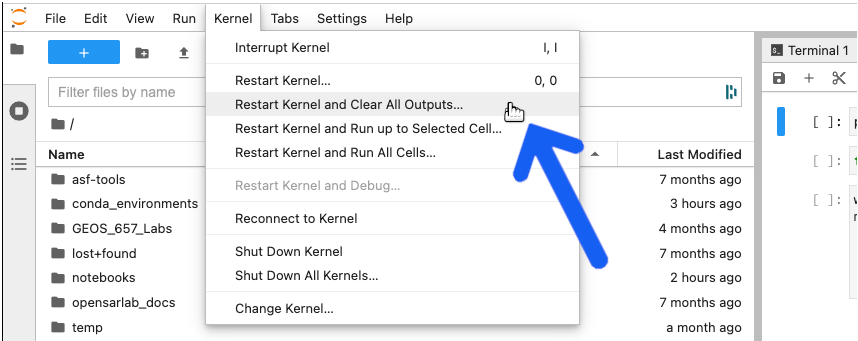
\includegraphics[width=0.7\linewidth]{files/restart_clear_all_jl-69996a882d58b2b807efb0170b60c542.png}
\caption*{Select \texttt{Restart Kernel and Clear All Outputs} from the \texttt{Kernel} menu and try saving it again.}
\end{figure}


\bigskip
\centerline{\rule{13cm}{0.4pt}}
\bigskip

\subsubsection{I am receiving a \texttt{No space left on device} error.}\label{I-am-receiving-a-No-space-left-on-device-error}

OpenSARLab users have access to a finite amount of storage space (\href{OpenSARlab\_environment.md}{details here}).

\textbf{It is up to users to manage their storage}.

\begin{itemize}
\item If you receive a storage space warning while logged into OpenSARlab, it is highly recommended to free up your space immediately by deleting unnecessary files. If your server shuts down without any available space, it will not have enough space on your volume to restart again and you will be locked out of your account.


\item If you do get locked out from your account, contact an \href{mailto:uaf-jupyterhub-asf@alaska.edu}{OpenSARlab administrator} for help.
\end{itemize}


\bigskip
\centerline{\rule{13cm}{0.4pt}}
\bigskip

\subsubsection{My server won't start and I cannot access OpenSARlab.}\label{My-server-wont-start-and-I-cannot-access-OpenSARlab}

This issue is typically due either to an unexpected behavior of \href{https://jupyterhub.github.io/nbgitpuller/}{nbgitpuller} or to having used up all space on your storage volume.

Please contact an \href{mailto:uaf-jupyterhub-asf@alaska.edu}{OpenSARlab Administrator} for help.


\bigskip
\centerline{\rule{13cm}{0.4pt}}
\bigskip

\subsubsection{The edits I made to an ASF notebook have disappeared since the last time I used OpenSARlab.}\label{The-edits-I-made-to-an-ASF-notebook-have-disappeared-since-the-last-time-I-used-OpenSARlab}

\begin{itemize}
\item When your OpenSARlab server starts up, \texttt{nbgitpuller} runs and pulls in any updates made to the \href{https://github.com/asfadmin/asf-jupyter-notebooks}{asf-jupyter-notebooks} and other Jupyter Book GitHub repositories provided in OpenSARLab. If a change has been made to a notebook by both the user and the author, both changes will be saved. The author's updated version will retain its original name while the user's version will have a timestamp appended to its name.
\end{itemize}

\begin{framed}
\textbf{Example file naming format for updated notebooks synched with \texttt{nbgitpuller}}\\
Notebook containing new updates: \texttt{sample\_notebook.ipynb}

Notebook previously edited by user, now with a timestamp appended to the name: \texttt{sample\_notebook\_20240616165846.ipynb}
\end{framed}

\begin{itemize}
\item If you think your notebook is missing, it is likely in its original location with a recent timestamp appended to its name.
\end{itemize}


\bigskip
\centerline{\rule{13cm}{0.4pt}}
\bigskip

\subsubsection{One of my notebooks looks like it has a mix of code from various versions of the notebook.}\label{One-of-my-notebooks-looks-like-it-has-a-mix-of-code-from-various-versions-of-the-notebook}

\begin{itemize}
\item We have seen this happen occasionally and it is caused by \href{https://jupyterhub.github.io/nbgitpuller/}{nbgitpuller}. The best option is to delete the notebook and \href{restarting\_server\_and\_kernel.md}{restart your OpenSARlab server}. The notebook will be replaced with a fresh copy from its nbgitpuller-managed repository.
\end{itemize}


\bigskip
\centerline{\rule{13cm}{0.4pt}}
\bigskip

\subsubsection{I am having trouble setting up a web server and developing my web app in OpenSARlab.}\label{I-am-having-trouble-setting-up-a-web-server-and-developing-my-web-app-in-OpenSARlab}

\begin{itemize}
\item This cannot be done in OpenSARlab. You will need to do this elsewhere.
\end{itemize}


\bigskip
\centerline{\rule{13cm}{0.4pt}}
\bigskip

\subsubsection{A notebook won't load. A new browser tab opens and shows the JupyterHub header, but no notebook appears.}\label{A-notebook-wont-load-A-new-browser-tab-opens-and-shows-the-JupyterHub-header-but-no-notebook-appears}

\begin{itemize}
\item This is due to slow loading time caused by a large notebook.


\item If you run a notebook and close it without clearing all output from the code cells, the file size will increase. This may cause it to load very slowly, depending on a user's network bandwidth.

\begin{itemize}
\item \textit{A 40KB notebook can grow to over 60MB if you don't clear its output.}
\end{itemize}


\item Try clearing the notebook's output before opening it by running the following command in the terminal:

\begin{itemize}
\item \texttt{jupyter nbconvert --clear-output --inplace my\_notebook.ipynb}
\end{itemize}
\end{itemize}


\bigskip
\centerline{\rule{13cm}{0.4pt}}
\bigskip

\subsubsection{My issue is not on this list}\label{My-issue-is-not-on-this-list}

\begin{itemize}
\item Please contact an \href{mailto:uaf-jupyterhub-asf@alaska.edu}{OpenSARlab administrator} for help.
\end{itemize}

%  TODO: add documentation in regards to server timeouts

\section{User Guide}

\subsection{OpenScienceLab and OpenSARLab Accounts}

\begin{itemize}
\item \href{/opensciencelab-accounts}{OpenScienceLab Accounts}
\item \href{/opensarlab-accounts}{OpenSARLab Accounts}
\item \href{/custom-deployment-access}{Class and Custom Labs}
\item \href{/mfa}{Configuring and Resetting MFA}
\item \href{/reset-password}{Resetting your OpenScienceLab Password}
\end{itemize}

\subsubsection{OpenScienceLab Accounts}

\newline
OpenScienceLab is a single-sign-on portal providing access to ASF-managed JupyterHubs such as OpenSARLab. OpenScienceLab also hosts labs for research projects, classes, and workshops. If you are attending a class or workshop, your instructor will provide details for gaining access to the lab.

\begin{framed}
\textbf{Note}\\
ASF provides limited access to OpenSARLab. NASA-affiliates are granted access upon \href{mailto:uso@asf.alaska.edu?subject=NASA-affiliate\%20OSL\%20access\%20request}{request}. All others may apply for access by completing the OpenSARLab Access Application
\end{framed}

\begin{framed}
\textbf{Tip}\\
Labs in OpenScienceLab are independent and do not share resources:

\begin{itemize}
\item If you have access to multiple labs, each will have its own storage volume and you cannot copy data directly from one to another.
\item Be mindful to use the correct lab for a given event. They are configured to support expected workflows.
\end{itemize}
\end{framed}


\bigskip
\centerline{\rule{13cm}{0.4pt}}
\bigskip

\paragraph{Sign Up for an OpenScienceLab Account}

\textbf{Whether accessing OpenSARLab, a class/workshop lab, or any other ASF-hosted lab, you will need an OpenScienceLab account}

\begin{enumerate}
\item Open a web browser and navigate to \href{https://opensciencelab.asf.alaska.edu/}{https://opensciencelab.asf.alaska.edu/}


\item
\end{enumerate}

\begin{figure}[!htbp]
\centering
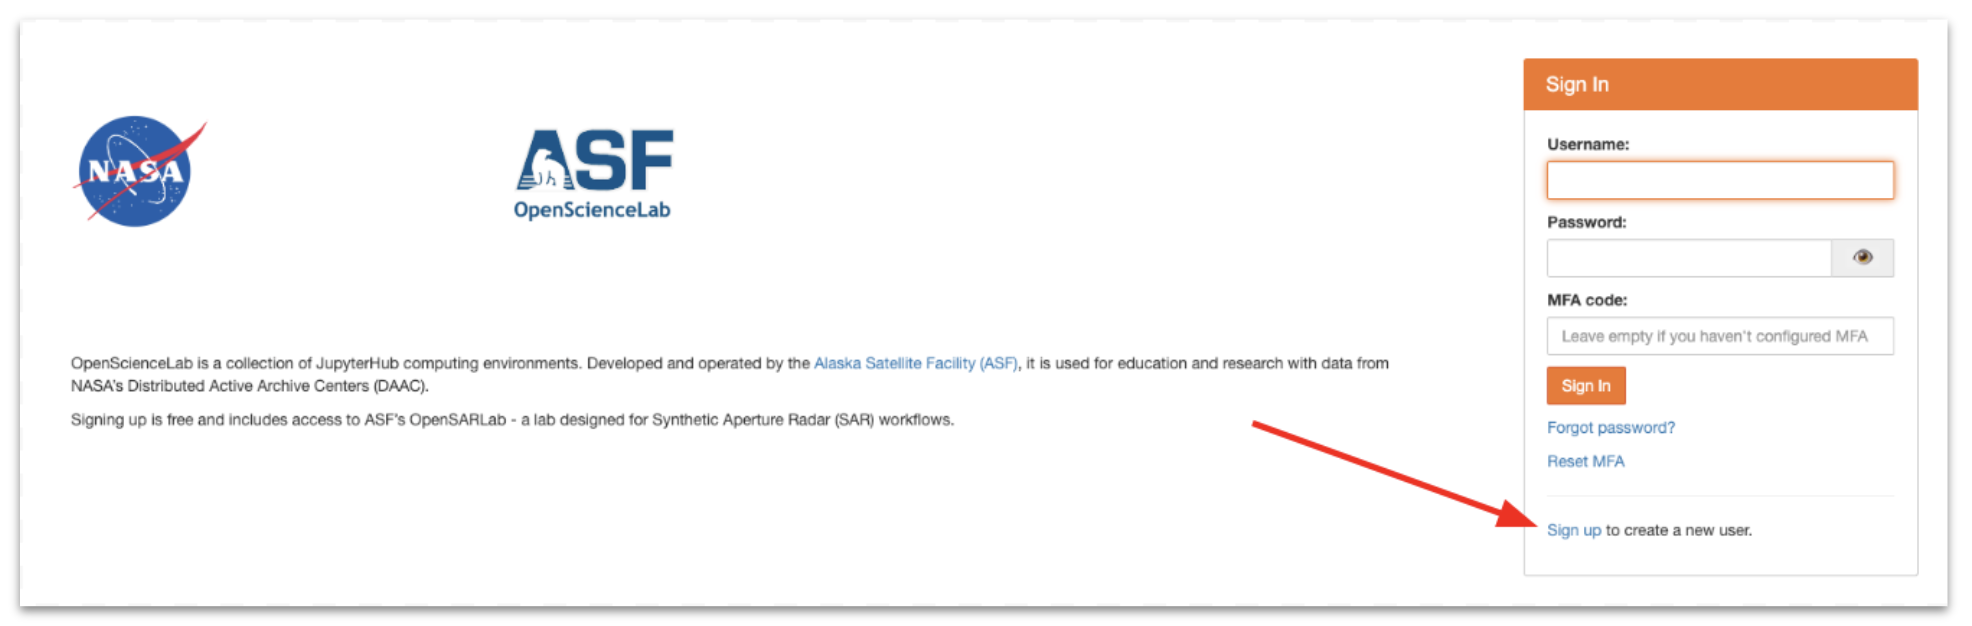
\includegraphics[width=0.35\linewidth]{files/opensciencelab_login-182d22b9a0b2d9fcf3f0497d8fc73446.png}
\caption*{Click the ``Sign up'' link in the ``Sign In'' window}
\end{figure}

\begin{enumerate}[resume]
\item
\end{enumerate}

\begin{figure}[!htbp]
\centering
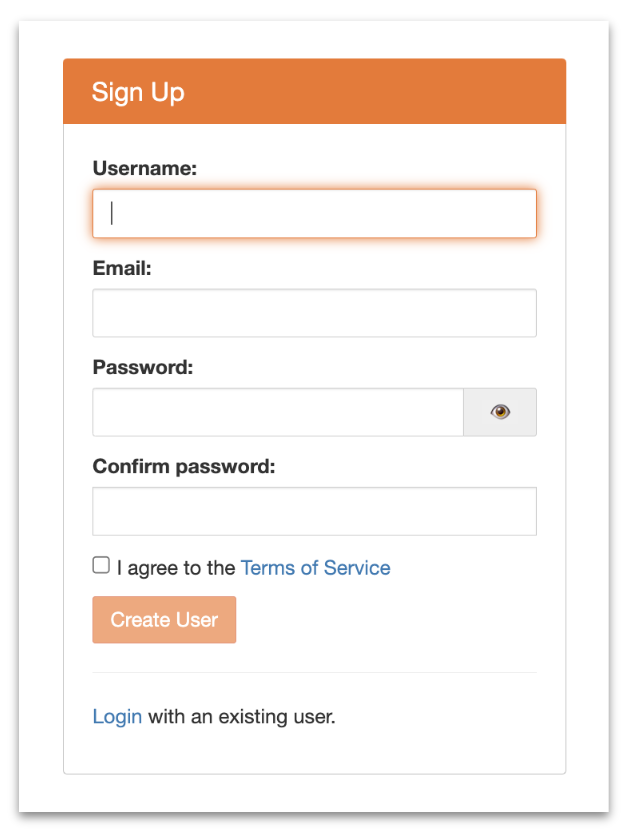
\includegraphics[width=0.35\linewidth]{files/opensciencelab_sign_-f6c8080ecc9648edb82f34b9742eafff.png}
\caption*{Complete the Sign Up form}
\end{figure}

\begin{enumerate}[resume]
\item
\end{enumerate}

\begin{figure}[!htbp]
\centering
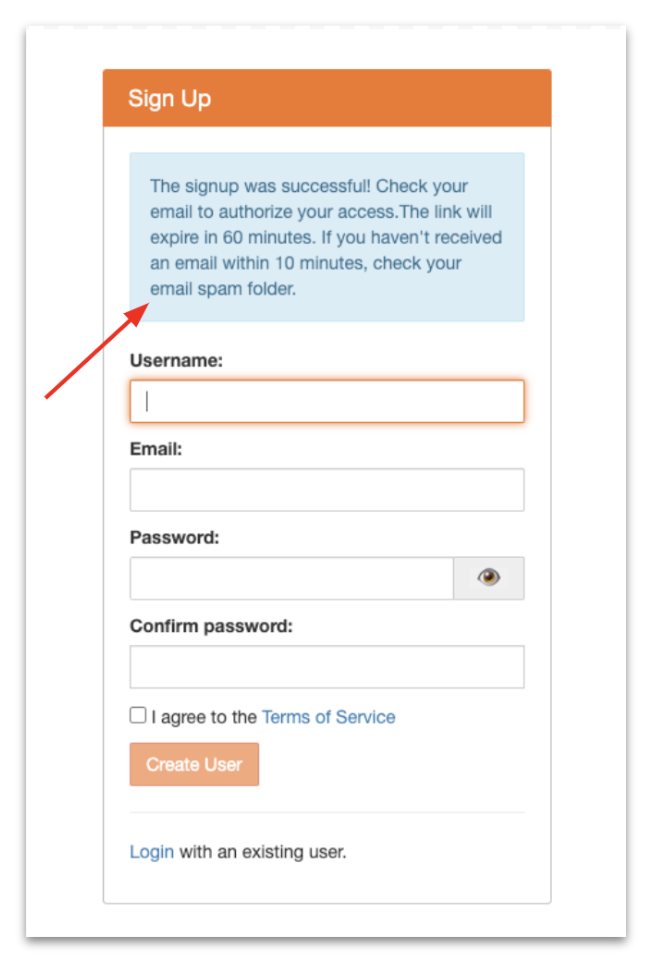
\includegraphics[width=0.35\linewidth]{files/opensciencelab_signu-13212f4d6228b42bd64ba31e65a3b336.png}
\caption*{A message will appear, indicating that your account was created and that email authorization is required. Locate the email and click the link within 60 minutes. If you don't click the link in time, you can start the sign up process over with a different username or contact OpenScienceLab admin and request a reset so you can try again with the same username.}
\end{figure}

\begin{enumerate}[resume]
\item
\end{enumerate}

\begin{figure}[!htbp]
\centering
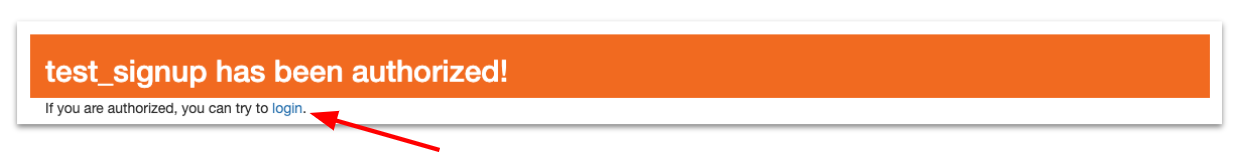
\includegraphics[width=1\linewidth]{files/opensciencelab_auth_-98494d5673ebf543d8e5c917aae4c819.png}
\caption*{The authorization link will open to a message indicating successful account authorization. You can click the include link to login.}
\end{figure}

\begin{enumerate}[resume]
\item Do not provide an MFA code the first time you login; leave the field blank. You will be required to setup MFA after signing in the first time in order to access any labs. MFA~setup~instructions.
\end{enumerate}

\subsubsection{OpenSARLab Accounts}

\newline
OpenSARLab is a cloud-hosted JupyterHub configured for working with SAR data. It is deployed next to NASA data in AWS region us-west-2 for low-latency access to large SAR datasets.

\begin{itemize}
\item Access~to~OpenSARLab
\item Account~Lifecycle
\item OpenSARLab~Environment
\end{itemize}


\bigskip
\centerline{\rule{13cm}{0.4pt}}
\bigskip

\paragraph{Access to OpenSARLab}\label{Access-to-OpenSARLab}

ASF provides limited access to OpenSARLab.

\begin{itemize}
\item NASA-affiliates are granted access upon \href{mailto:uso@asf.alaska.edu?subject=NASA-affiliate\%20OSL\%20access\%20request}{request}.
\item All others may apply for access by completing the \href{https://forms.gle/LNBCwe8JohYitvfy6}{OpenSARLab Access Application}.
\end{itemize}


\bigskip
\centerline{\rule{13cm}{0.4pt}}
\bigskip

\paragraph{Account Lifecycle}\label{Account-Lifecycle}

\begin{itemize}
\item Accounts will be deactivated on the \textbf{30th} day of inactivity.
\item Warning emails are sent to inactive users after \textbf{29}, \textbf{27}, and \textbf{24} days.
\item The user volume and snapshot are \textbf{permanently destroyed} upon account deactivation.
\end{itemize}

\textit{Lifecycle periods for custom labs may differ.}


\bigskip
\centerline{\rule{13cm}{0.4pt}}
\bigskip

\paragraph{OpenSARLab Environment}\label{OpenSARLab-Environment}

\subparagraph{Operating System}

\begin{itemize}
\item Ubuntu 22.04.4 LTS
\end{itemize}

\subparagraph{Server Profiles}

Every OpenSARLab user has access to a JupyterHub server running on an AWS EC2 instance. Users may select from two server profiles offering varying amounts of compute resources to support different workloads.

\begin{quote}
\textbf{m6a.large:}

\begin{itemize}
\item RAM Guarantee: 5G
\item RAM limit: 8G
\item CPU limit: 2
\end{itemize}

\textbf{m6a.xlarge:}

\begin{itemize}
\item RAM Guarantee: 10G
\item RAM limit: 16G
\item CPU limit: 4
\end{itemize}
\end{quote}

\subparagraph{Volume (storage)}

\begin{itemize}
\item *500GB of EBS volume storage per user.
\end{itemize}

OpenSARLab uses \href{https://docs.aws.amazon.com/AWSEC2/latest/UserGuide/ebs-volumes.html}{Amazon AWS EBS volumes} mounted on user servers' home directories for persistent storage.

\begin{itemize}
\item If a volume is full when a user shuts down their server, it will trigger an \texttt{out-of-storage exception} that will prevent users from starting a server again.\begin{itemize}
\item Please contact an \href{mailto:uaf-jupyterhub-asf@alaska.edu}{OpenScienceLab administrator} if this occurs.
\end{itemize}
\end{itemize}

\subparagraph{\textbf{Privileges}}

\begin{itemize}
\item Users do not have \texttt{root} (i.e., \texttt{sudo}) privileges.
\item Users have read/write access in their local directories on their EBS volumes, but limited write access in their root directories.
\end{itemize}

\subsubsection{Class and Custom Labs}

\newline
Custom labs are created for specific uses, such as hosting a class or a research team working on a project.

\paragraph{Cloud Resources in Custom Labs}

The resources provided in custom labs are based on the anticipated needs of a given user group and often differ from those provided in OpenSARLab. Requests for changes to compute and storage resources must be approved by the owner of a custom lab. This is typically a professor, workshop host, or PI on a grant-funded project.

\paragraph{Custom Lab Access}

Access to all custom labs is determined by the owner of each lab. Professors, instructors, or PIs should provide instructions for accessing a custom lab. Access will require an \href{/opensciencelab-accounts}{OpenScienceLab account}.

Once a user's OpenScienceLab account has been given access to a lab, a lab access card will appear in the OpenScienceLab portal after signing in.

\begin{figure}[!htbp]
\centering
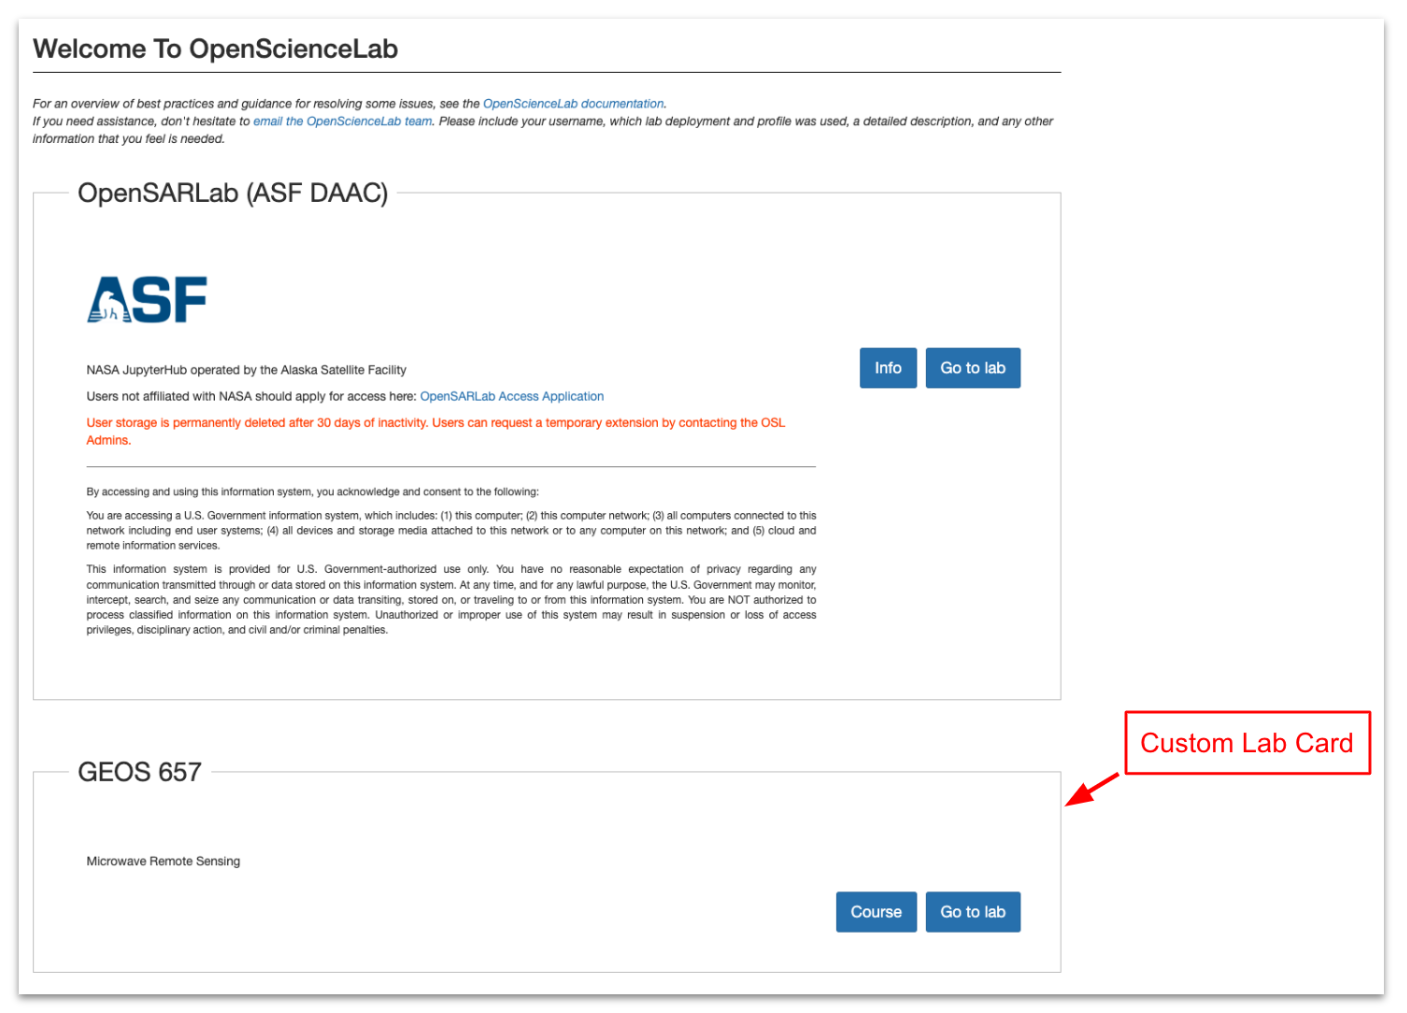
\includegraphics[width=0.7\linewidth]{files/opensciencelab_custo-3c1a84de52b386ba0c769f8989eeccea.png}
\caption*{OpenScienceLab with custom lab card}
\end{figure}

\subsubsection{Configuring and Resetting MFA}

\newline
Multi-Factor Authentication (MFA) is required to access OpenScienceLab resources.

Currently, we support TOTP-based authentication, with plans to add hardware
key (ex. Yubikey) authentication in future updates.

\begin{itemize}
\item Watch:~Log~In~and~Set~Up~MFA
\item Before~You~Begin
\item Setup~Steps
\item Resetting~MFA
\item Troubleshooting
\end{itemize}


\bigskip
\centerline{\rule{13cm}{0.4pt}}
\bigskip

\paragraph{Watch: Log In and Set Up MFA}\label{Watch-Log-In-and-Set-Up-MFA}


\bigskip
\centerline{\rule{13cm}{0.4pt}}
\bigskip

\paragraph{Before You Begin}\label{Before-You-Begin}

A TOTP-enabled MFA application is required to use OpenScienceLab resources.
While the most widely utilized approach is through a smartphone application,
there are also several desktop clients that provide this functionality.

\begin{framed}
\textbf{MFA App Support}\\
\bigskip\noindent
\begin{tabular}{p{\dimexpr 0.250\linewidth-2\tabcolsep}p{\dimexpr 0.250\linewidth-2\tabcolsep}p{\dimexpr 0.250\linewidth-2\tabcolsep}p{\dimexpr 0.250\linewidth-2\tabcolsep}}
\toprule
Application & Desktop Support & Android Support & iOS Support \\
\hline
KeePassXc & ✅ & ❌ & ❌ \\
Enpass & ✅ & ✅ & ✅ \\
Cisco Duo & ✅ & ✅ & ✅ \\
\href{http://Authenticator.cc}{Authenticator.cc}* & ✅ & ✅ & ✅ \\
Bitwarden** & ✅ & ✅ & ✅ \\
FreeOTP & ❌ & ✅ & ✅ \\
Google Authenticator & ❌ & ✅ & ✅ \\
Microsoft Authenticator & ❌ & ✅ & ✅ \\
Aegis Authenticator & ❌ & ✅ & ❌ \\
\bottomrule
\end{tabular}

\bigskip* Browser based

** TOTP supported in paid version only
\end{framed}


\bigskip
\centerline{\rule{13cm}{0.4pt}}
\bigskip

\paragraph{Setup Steps}\label{Setup-Steps}

\begin{enumerate}
\item Log into OpenScienceLab normally. Leave the ``MFA'' field on the login page blank.
\item Click ``Configure New MFA Device'' in the Navigation Bar at
the top of the page.
\item Configure your MFA device:\begin{enumerate}
\item If using a smartphone application, scan the QR code using the
application's ``Scan QR Code'' feature.
\item If using a desktop application, copy the OTP Secret into the ``TOTP'' field
\end{enumerate}


\item Enter the current 6-digit MFA code generated by your application into the ``Code 1'' field
on the ``Configure New MFA Device'' page.
\item When the code changes, enter the new code into the ``Code 2'' field on the same
page and click the ``Check MFA Codes'' button.
\item If the check is successfull, navigate back to the home page by clicking ``Home''
in the Navigation Bar at the top of the page and continue using OpenScienceLab
as normal.
\end{enumerate}


\bigskip
\centerline{\rule{13cm}{0.4pt}}
\bigskip

\paragraph{Resetting MFA}\label{Resetting-MFA}

On occasion, you may wish or need to reconfigure MFA for your OSL account.

\begin{enumerate}
\item Navigate to \href{https://opensciencelab.asf.alaska.edu/}{opensciencelab}.


\item
\end{enumerate}

\begin{figure}[!htbp]
\centering
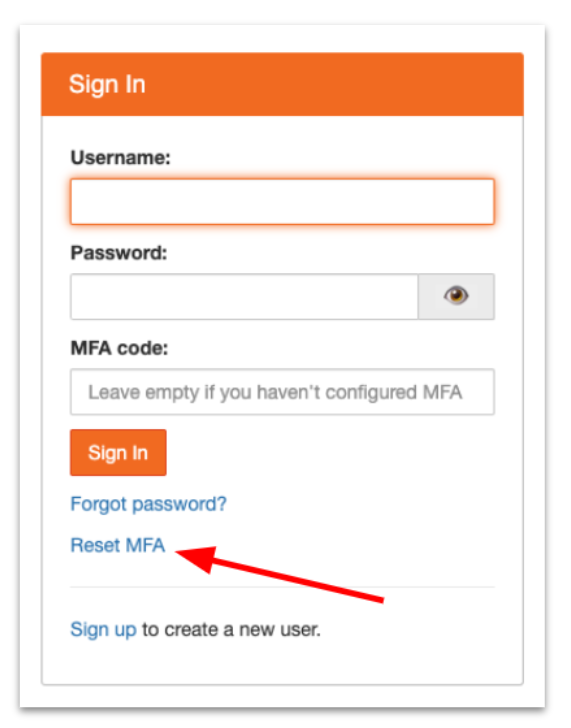
\includegraphics[width=0.4375\linewidth]{files/reset_mfa-236175c67c558a74caf5dfff2036ca1a.png}
\caption*{Click the "Reset MFA" link on the sign in card}
\end{figure}

\begin{enumerate}[resume]
\item
\end{enumerate}

\begin{figure}[!htbp]
\centering
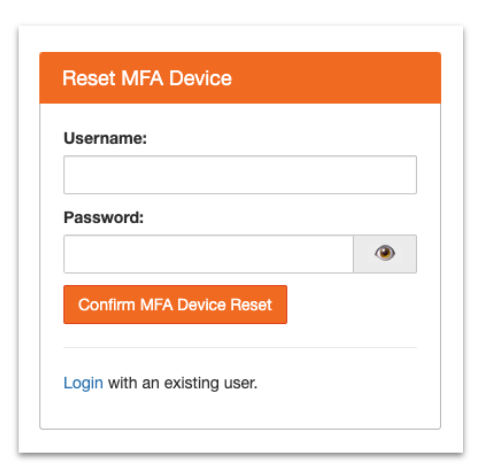
\includegraphics[width=0.4375\linewidth]{files/mfa_reset_form-ca56fa832e366f636d3f2771f45e7255.png}
\caption*{Complete the MFA reset form.}
\end{figure}

\begin{enumerate}[resume]
\item
\end{enumerate}

\begin{figure}[!htbp]
\centering
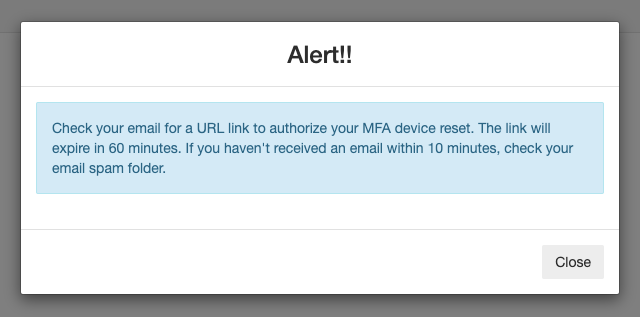
\includegraphics[width=0.625\linewidth]{files/mfa_update_alert-3e0a0f153977a430edaea4ff25e7887d.png}
\caption*{An alert will appear directing you to click an emailed verification link within 60 minutes.}
\end{figure}

\begin{enumerate}[resume]
\item
\end{enumerate}

\begin{figure}[!htbp]
\centering
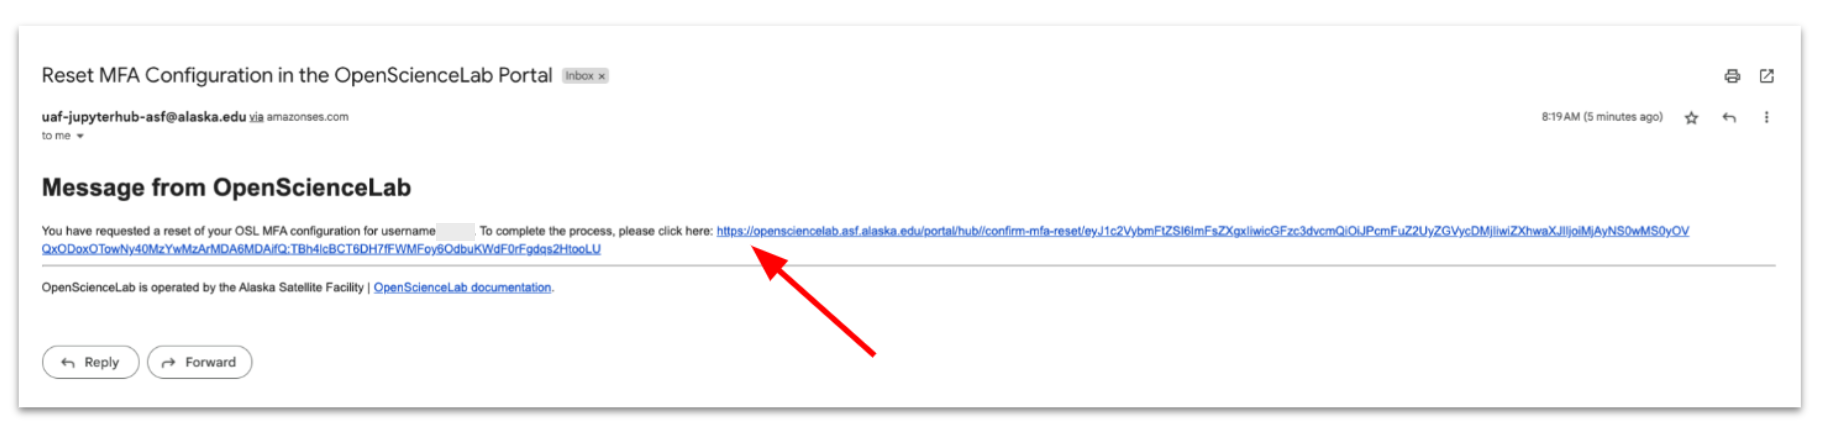
\includegraphics[width=0.7\linewidth]{files/mfa_reset_email-c0d983a161cc3d91309ff3be25196636.png}
\caption*{Click the verification link in the email.}
\end{figure}

\begin{enumerate}[resume]
\item Sign into OpenScienceLab, leaving the MFA field empty.
\item \textbf{Follow the Setup Steps above to setup a new MFA device.} You will not be able to access any labs until you setup a new MFA device.
\end{enumerate}


\bigskip
\centerline{\rule{13cm}{0.4pt}}
\bigskip

\paragraph{Troubleshooting}\label{Troubleshooting}

\begin{enumerate}
\item If the MFA Code check is not successful, there are two potential issues:\begin{enumerate}
\item One of the codes was mis-typed.
\item The secret was not properly put into the MFA application.
\end{enumerate}


\item Test again with another two \textit{consecutive} codes, and if the verification step fails
again, check that the OTP Secret on the page matches the secret in your application.
\item If all else fails, refresh the page. This will generate a new code, which you
can then use to follow the same steps above.
\end{enumerate}

For additional issues and further troubleshooting, please email
\href{mailto:uso@asf.alaska.edu}{uso@asf.alaska.edu}

\subsubsection{Resetting Your OpenScienceLab Password}

\begin{enumerate}
\item
\end{enumerate}

\begin{figure}[!htbp]
\centering
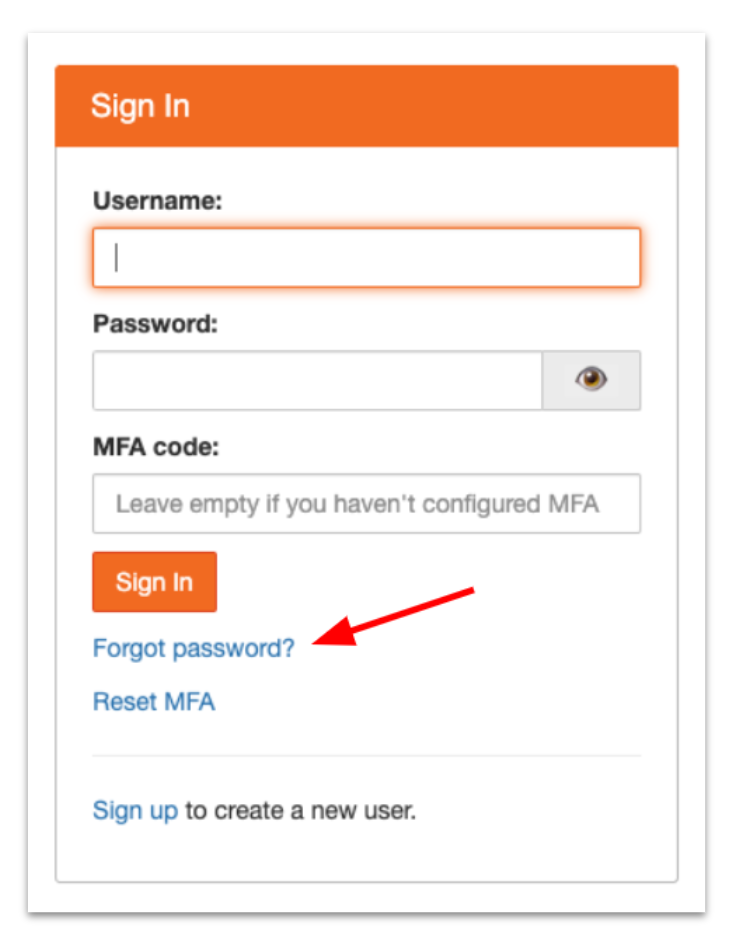
\includegraphics[width=0.4375\linewidth]{files/opensciencelab_pass_-b77580f7b43d7043b0d9aeba9100ddd6.png}
\caption*{Navigate to \href{https://opensciencelab.asf.alaska.edu/}{OpenScienceLab} and click the "Forgot password?" link on the sign in section.}
\end{figure}

\begin{enumerate}[resume]
\item
\end{enumerate}

\begin{figure}[!htbp]
\centering
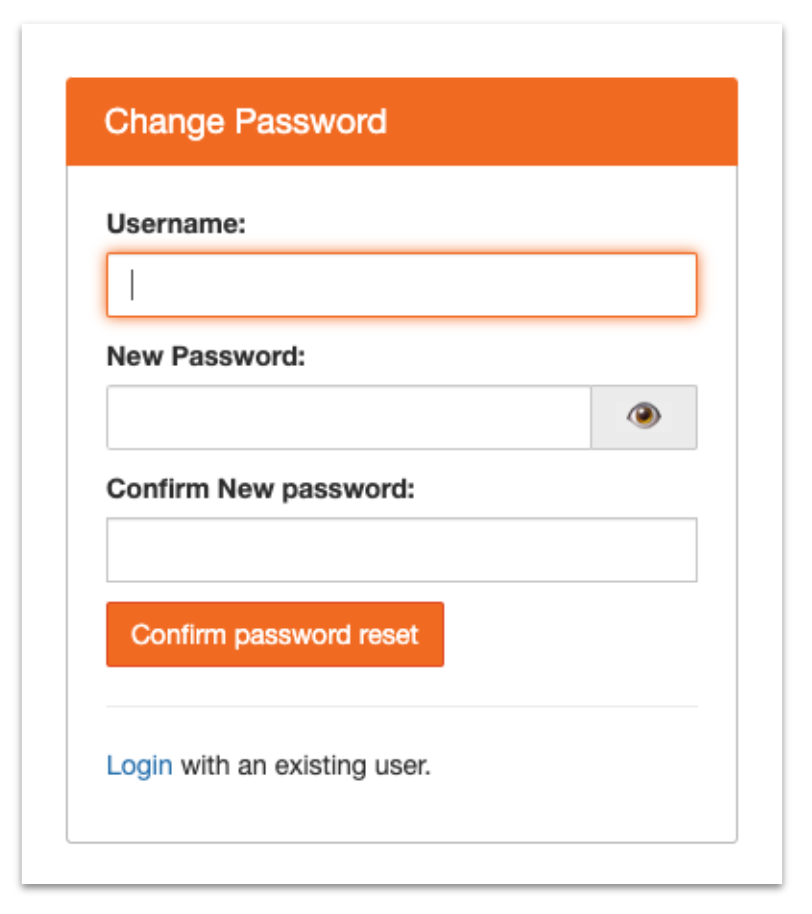
\includegraphics[width=0.4375\linewidth]{files/opensciencelab_chang-79bf27a5ab0f86a7cc0426cbaa14c19e.png}
\caption*{Complete and submit the Change Password form.}
\end{figure}

\begin{enumerate}[resume]
\item
\end{enumerate}

\begin{figure}[!htbp]
\centering
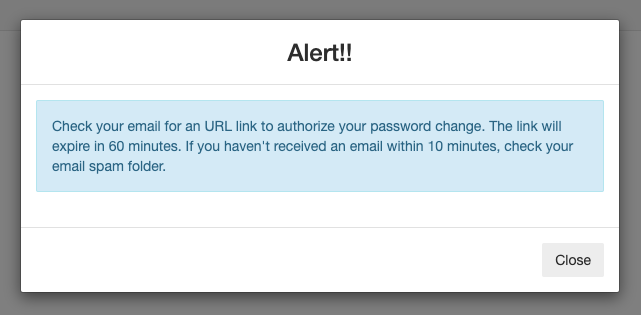
\includegraphics[width=0.625\linewidth]{files/opensciencelab_pass_-b21cd947a10fda3e22b3b87ee927ea19.png}
\caption*{An alert will appear directing you to click the emailed verification link within 60 minutes.}
\end{figure}

\begin{enumerate}[resume]
\item
\end{enumerate}

\begin{figure}[!htbp]
\centering
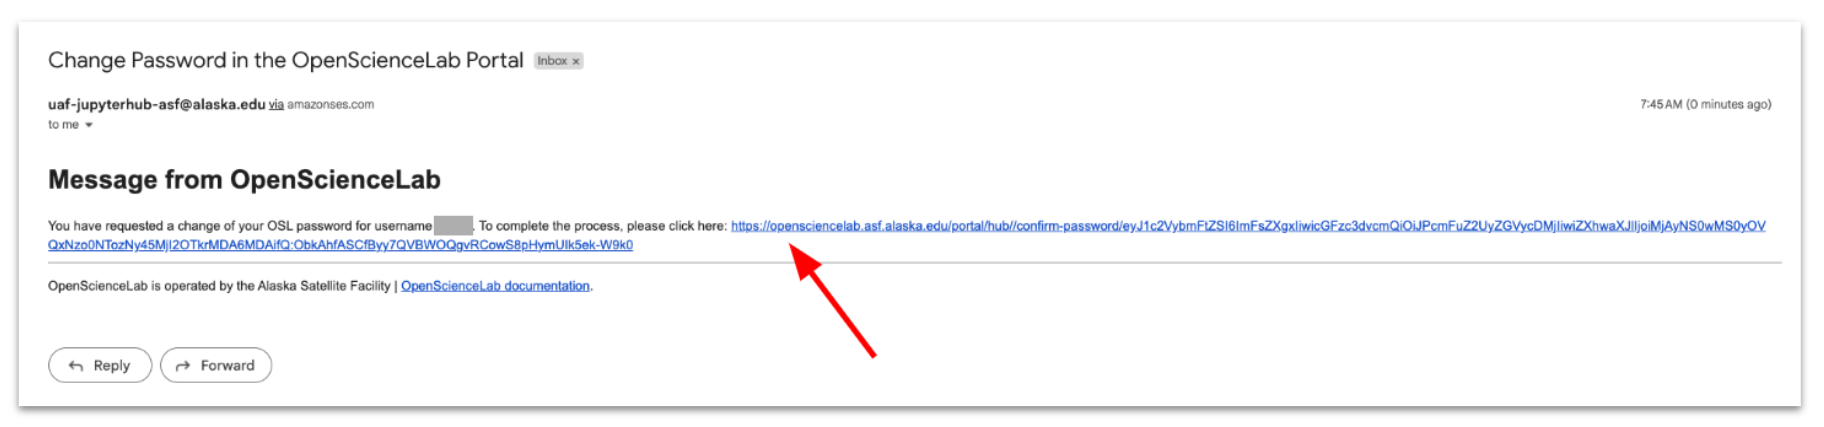
\includegraphics[width=0.7\linewidth]{files/opensciencelab_passw-dcdf0b6f219deac5a2f0fde3c562af74.png}
\caption*{Open the email and click the verification link.}
\end{figure}

\begin{enumerate}[resume]
\item Log into OpenScienceLab with your new credentials.
\end{enumerate}

\subsection{JupyterLab and Jupyter Notebooks}

\begin{itemize}
\item \href{/how-to-run-a-notebook}{Running Jupyter Notebooks}
\item \href{/jupyter-magic}{Jupyter Magic Commands}
\item \href{/class-notebooks-best-practices}{Notebook Development Best Practices}
\item \href{/jupyter-servers}{JupyterLab Servers}
\item \href{/jupyter-kernels}{Jupyter Notebook Kernels}
\item \href{/opensarlab-terminal}{Jupyter Terminal}
\item \href{/logging-out-and-server-shutdown}{Server/Logout Shutdown Best Practices}
\item \href{/jupyterlab-extensions}{JupyterLab Extensions}
\end{itemize}

\subsubsection{Running Jupyter Notebooks}

\newline
\href{https://docs.jupyter.org/en/latest/}{Jupyter Notebooks} allow users to display:

\begin{itemize}
\item Interactive and runnable code cells, typically written in \href{https://docs.python.org/3/}{Python}
\item \href{https://jupyter-notebook.readthedocs.io/en/stable/examples/Notebook/Working\%20With\%20Markdown\%20Cells.html}{Markdown} cells containing explanatory text, formulas, hyperlinks, tables, pseudocode, images, etc.
\end{itemize}

Jupyter Notebooks provide an ideal file format for teaching/learning coding concepts and prototyping algorithms.


\bigskip
\centerline{\rule{13cm}{0.4pt}}
\bigskip

\begin{itemize}
\item Notebook~Cell~Types\begin{itemize}
\item Markdown~Cells
\item Code~Cells
\end{itemize}


\item How~to~Run~Jupyter~Notebooks\begin{itemize}
\item Selecting~Cells\begin{itemize}
\item Select~an~Individual~Cell
\item Select~Multiple~Cells
\end{itemize}


\item Hide~Code~Cells\begin{itemize}
\item Collapse~an~Individual~Cell
\item Collapse~Selected~Cells~or~All~Cells~in~a~Notebook
\item Hide~Sections~of~Code~Cells~beneath~a~Markdown~Cell
\end{itemize}


\item Running~Code~Cells\begin{itemize}
\item Run~a~Single~Code~Cell
\item Run~Multiple~Code~Cells\begin{itemize}
\item Run~a~batch~of~selected~cells
\item Run~Every~Cell~Above~or~Below~a~Code~Cel
\item Run~an~Entire~Notebook
\end{itemize}


\item Rerunning~a~Notebook
\end{itemize}


\item Clearing~Cell~Output~Before~Closing
\end{itemize}
\end{itemize}


\bigskip
\centerline{\rule{13cm}{0.4pt}}
\bigskip

\paragraph{Notebook Cell Types}\label{Notebook-Cell-Types}

\subparagraph{Markdown Cells}\label{markdown-cells}

Markdown cells contain documentation in Markdown, MyST Markdown, HTML, and/or LaTeX. They are often used to display text, images, hyperlinks, formulas, tables, pseudocode, plots, figures, etc.

\textbf{Markdown Edit Mode}

To enter edit mode in a markdown cell, double-click the cell.

\begin{figure}[!htbp]
\centering
\includegraphics[width=0.7\linewidth]{files/markdown_cell_edit_m-b8e8c5b3b1cc0a471bb3ae84ec951803.gif}
\caption*{Double-click on a markdown cell to enter edit mode}
\end{figure}

\textbf{Markdown Display Mode}

To render a markdown cell, select it then:

\begin{itemize}
\item Click the \textbf{play} button at the top of the notebook
\end{itemize}

or

\begin{itemize}
\item Use the \texttt{shift + enter} ``play'' shortcut.
\end{itemize}

\begin{figure}[!htbp]
\centering
\includegraphics[width=0.7\linewidth]{files/markdown_run-0dba41b32d4680b49aeb935ccbacf54e.gif}
\caption*{A run markdown cell}
\end{figure}

\subparagraph{Code Cells}\label{code-cells}

Code cells contain editable and runnable Python code. You can run them sequentially or in any order, once or any number of times.

\begin{figure}[!htbp]
\centering
\includegraphics[width=0.7\linewidth]{files/code_cell-626391938035d549c42fc8ffc2ea829b.gif}
\caption*{Selecting and running a code cell}
\end{figure}

\begin{framed}
\textbf{Tip}\\
While the ability to rerun the code cells in arbitrary order can be helpful, it can also cause problems, such as:

\begin{itemize}
\item Recycled variables may contain unexpected values if you run cells in non-sequential order.
\item You may skip cells that set required variables or perform necessary functions.
\item If you change directories in a code cell and run other cells in an unexpected order, you could attempt to run code in the wrong location.
\end{itemize}
\end{framed}


\bigskip
\centerline{\rule{13cm}{0.4pt}}
\bigskip

\paragraph{How to Run Jupyter Notebooks}\label{How-to-Run-Jupyter-Notebooks}

\subparagraph{Selecting Cells}\label{selecting-cells}

Users may select cells individually or in a batch, and then run the selected cells.

\subparagraph{Select an Individual Cell}\label{Select-an-Individual-Cell}

\begin{itemize}
\item Click anywhere inside a cell to select it.
\end{itemize}

\begin{figure}[!htbp]
\centering
\includegraphics[width=0.7\linewidth]{files/select_cells-d971b876354f6e0a79598cad2bd78f12.gif}
\caption*{A selected cell displays a blue vertical line on the left edge.}
\end{figure}

\subparagraph{Select Multiple Cells}\label{Select-Multiple-Cells}

\begin{enumerate}
\item Select a cell \textbf{by clicking to the left of the text box}\begin{itemize}
\item Clicking inside the cell will select it but it will place you in text edit mode and you will not be able to select additonal cells.
\end{itemize}


\item Select additional cells using:\begin{itemize}
\item \texttt{shift + j} or \texttt{shift + Down-Arrow} to select additional cells below
\item \texttt{shift + k} or \texttt{shift + Up-Arrow} to select additional cells above
\item \texttt{shift + mouse click} to select batches of cells
\end{itemize}


\item Perform batch operations on selected cells with \textbf{\texttt{▶}} button or with \texttt{Ctrl + Enter} or \texttt{Cmd + Enter} (Mac).
\end{enumerate}

\begin{figure}[!htbp]
\centering
\includegraphics[width=0.7\linewidth]{files/select_multiple_cell-6769ad25c2c6800ce81fc8df5fa716a7.gif}
\caption*{Selected cells will be surrounded by a blue background}
\end{figure}

\subparagraph{Hide Code Cells}\label{Hide-Code-Cells}

You may occasionally wish to hide code cells to reduce clutter.

\subparagraph{Collapse an Individual Cell}\label{Collapse-an-Individual-Cell}

\begin{figure}[!htbp]
\centering
\includegraphics[width=0.7\linewidth]{files/collapse_code_cell-d0f4a096d2d9d5afe983964fa35a4743.gif}
\caption*{You can hide an individual code cell by clicking the blue vertical line to the left of the code cell.}
\end{figure}

\subparagraph{Collapse Selected Cells or All Cells in a Notebook}\label{Collapse-Selected-Cells-or-All-Cells-in-a-Notebook}

\begin{itemize}
\item Select some code cells and choose the menu option: \texttt{View} -\textgreater  \texttt{Collapse Selected Code}
\item Select the menu option: \texttt{View} -\textgreater  \texttt{Collapse All Code}
\end{itemize}

\subparagraph{Hide Sections of Code Cells beneath a Markdown Cell}\label{Hide-Sections-of-Code-Cells-beneath-a-Markdown-Cell}

\begin{figure}[!htbp]
\centering
\includegraphics[width=0.7\linewidth]{files/collapse_cells_under-e90f96c61cbff0e57c311440c9d799c7.gif}
\caption*{Hide entire sections of code cells beneath a markdown cell by clicking the vertical blue bar to the left of the markdown cell.}
\end{figure}


\bigskip
\centerline{\rule{13cm}{0.4pt}}
\bigskip

\paragraph{Running Code Cells}\label{running-code-cells}

Code cells may be executed in any order. A cell execution counter to the left of each code cell indicates the order in which the cells were run.

\begin{figure}[!htbp]
\centering
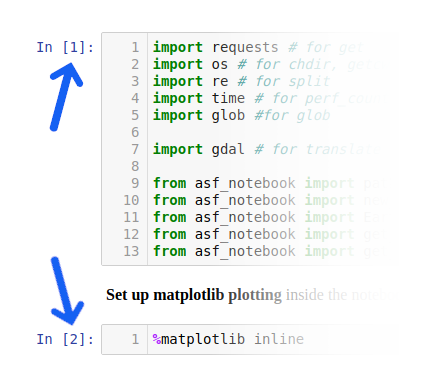
\includegraphics[width=0.7\linewidth]{files/cell_numbers-41fe16375e4710038066a4a0596391c8.png}
\caption*{The cell execution counter indicates the order in which code cells have run.}
\end{figure}

\subparagraph{Run a Single Code Cell}\label{run-a-single-code-cell}

\begin{enumerate}
\item Select the cell you wish to run.
\item Do one of the following:\begin{itemize}
\item Click the \texttt{▶} button at the top of the notebook.
\item \texttt{Ctrl + Enter} or \texttt{Cmd + Enter} (Mac) to run a cell.
\item \texttt{Shift + Enter} to run a cell and select the cell below
\item \texttt{Alt + Enter} to run a cell and insert an empty cell below
\end{itemize}
\end{enumerate}

\subparagraph{Run Multiple Code Cells}\label{Run-Multiple-Code-Cells}

\subparagraph{Run a batch of selected cells}\label{Run-a-batch-of-selected-cells}

\begin{enumerate}
\item Select a group of cells.
\item Do one of the following:\begin{itemize}
\item Click the \texttt{▶} button at the top of the notebook.
\item \texttt{Ctrl + Enter} to run a cell.
\item \texttt{Shift + Enter} to run a cell and select the cell below
\item \texttt{Alt + Enter} to run a cell and insert an empty cell below
\end{itemize}
\end{enumerate}

\subparagraph{Run Every Cell Above or Below a Code Cell}\label{Run-Every-Cell-Above-or-Below-a-Code-Cell}

Select a cell, then:

\begin{itemize}
\item Select the menu option: \texttt{Run} -\textgreater   \texttt{Run All Above Selected Cell}
\item Select the menu option: \texttt{Run} -\textgreater  \texttt{Run Selected Cell and All Below}
\end{itemize}

\subparagraph{Run an Entire Notebook}\label{Run-an-Entire-Notebook}

If you wish to run every code cell in a notebook, you can do one of the following:

\begin{itemize}
\item Select the menu option: \texttt{Run} -\textgreater  \texttt{Run All}
\item Select the menu option: \texttt{Kernel} -\textgreater  \texttt{Restart Kernel and Run All Cells...}
\end{itemize}

\begin{framed}
\textbf{Restarting the Kernel and Rerunning vs. Simply Rerunning}\\
Rerunning a notebook without restarting the kernel preserves previously defined local variables. This can potentially cause issues related to directory changes, paths, and variables containing unexpected values. It is generally safer to restart the kernel and rerun the notebook.
\end{framed}


\bigskip
\centerline{\rule{13cm}{0.4pt}}
\bigskip

\subparagraph{Rerunning a Notebook}\label{rerunning-a-notebook}

We recommend restarting the notebook kernel before rerunning it since any initialized variables and data structures from a previous run persist in memory along with their values, which can lead to unintended results.

To restart the kernel so you can begin a fresh notebook run use one of the following options:

\begin{itemize}
\item Select the menu option: \texttt{Kernel} -\textgreater  \texttt{Restart Kernel}
\item Select the menu option: \texttt{Kernel} -\textgreater  \texttt{Restart Kernel and Clear...}
\end{itemize}

\begin{framed}
\textbf{Clearing Notebook Output}\\
It is easy to lose track of your position in a notebook if it contains code cell output and execution counters from a previous run. We recommend clearing any output before rerunning a notebook.
\end{framed}


\bigskip
\centerline{\rule{13cm}{0.4pt}}
\bigskip

\paragraph{Clearing Cell Output Before Closing}\label{clearing-cell-output-before-closing}

For large notebooks with a lot of plots and images, we recommend clearing all code cell output before closing or saving a notebook. Leaving the output in place can increase the file size of the notebook, which can cause slower notebook loading times (especially if you have a slow internet connection).

\subsubsection{Jupyter Magic Commands}

\newline
In addition to running Python code, Jupyter Notebooks provide magic commands with various functions. We provide an introduction to a several, but many more are available. Plese see the \href{https://ipython.readthedocs.io/en/stable/interactive/magics.html}{Jupyter Magics documentaion} for more information.

\begin{itemize}
\item Shell~Assignment~Syntax
\item Line~Magics
\item Cell~Magics
\end{itemize}


\bigskip
\centerline{\rule{13cm}{0.4pt}}
\bigskip

\paragraph{Shell Assignment Syntax}\label{Shell-Assignment-Syntax}

In Jupyter Notebooks, the exclamation mark \texttt{!} allows users to run shell commands from inside a Jupyter Notebook code cell (\texttt{/bin/bash} in OpenSARLab).

Simply start a line of code with \texttt{!} and it will run the command in a shell, using the Conda environment of the currently running Python kernel.

\begin{figure}[!htbp]
\centering
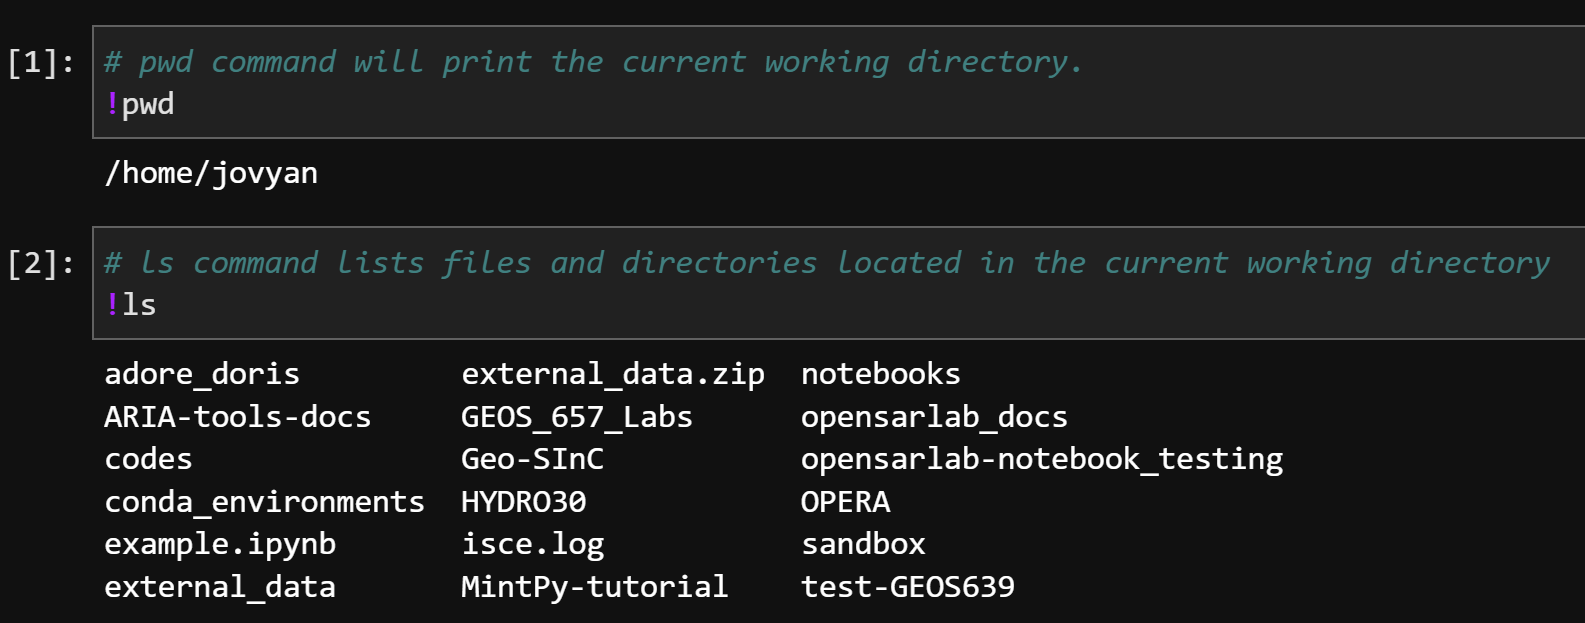
\includegraphics[width=0.7\linewidth]{files/magic_excl-12ba8e58141a58cf8b7fc5b21fa3c978.PNG}
\caption*{Using \texttt{!} to run shell commands in a Jupyter Notebook.}
\end{figure}


\bigskip
\centerline{\rule{13cm}{0.4pt}}
\bigskip

\paragraph{Line Magics}\label{Line-Magics}

Line magics start with a single \texttt{\%}. They either update a setting that affect the entire notebook or they affect only the line where \texttt{\%} is used.

\subparagraph{\texttt{\%matplotlib inline}}

\begin{itemize}
\item Display \textbf{non-interactive} \texttt{matplotlib plots} in code cell output.
\item Turns on inline plotting for the entire notebook
\end{itemize}

\subparagraph{\texttt{\%matplotlib widget}}

\begin{itemize}
\item Display \textbf{interactive} \texttt{matplotlib plots} in code cell output.
\item Turns on interactive plotting for the entire notebook.
\end{itemize}

\subparagraph{\texttt{\%time}}

\begin{itemize}
\item Time the execution of a Python expression.
\item Times only the line containing the \texttt{\%time} magic command.
\end{itemize}

\subparagraph{Find information on many more line magics \href{https://ipython.readthedocs.io/en/stable/interactive/magics.html\#:~:text=IPython\%20trove\%20classifier.-,Line\%20magics,-\%EF\%83\%81}{here}.}


\bigskip
\centerline{\rule{13cm}{0.4pt}}
\bigskip

\paragraph{Cell Magics}\label{Cell-Magics}

Cell magics start with \texttt{\%\%} and affect the contents of an entire code cell.

\subparagraph{\texttt{\%\%javascript} or \texttt{\%\%js}}

\begin{itemize}
\item Run a JavaScript code cell.
\end{itemize}

\begin{figure}[!htbp]
\centering
\includegraphics[width=0.7\linewidth]{files/magic_js-c34fba5a522f55637fc0723db6ae7d55.gif}
\caption*{Jupyter Javascript magic example.}
\end{figure}

\subparagraph{\texttt{\%\%capture}}

\begin{itemize}
\item Run a code cell but capture and hide all output.
\end{itemize}

\subparagraph{Find information on many more cell magics \href{https://ipython.readthedocs.io/en/stable/interactive/magics.html\#cell-magics:~:text=True\%20value\%20set.-,Cell\%20magics,-\%EF\%83\%81}{here}.}

\subsubsection{Notebook Development Best Practices}

\newline
\paragraph{Provide a Conda Environment Capable of Running the Notebooks}

\begin{itemize}
\item Include an \texttt{environment.yml} in your GitHub repository that can be used to build a Conda environment that supports the notebook.
\item Learn how to \href{/software}{Install software in a lab}.
\end{itemize}


\bigskip
\centerline{\rule{13cm}{0.4pt}}
\bigskip

\paragraph{Provide a Pinned \texttt{environment.yml} to Build a Conda Environment}

The open-source Python packages used in your Conda environments are routinely updated, often introducing breaking dependencies. If the \texttt{environment.yml} file does not pin packages to specific versions, the default behavior is to build the latest available versions. This can introduce new dependency conflicts at any time.

Even if you pin every package, there is still a risk that an \texttt{environment.yml} will no longer build correctly at some point. This can occur if one of its package versions is removed due to a security risk, legal issue, or the discovery of a critical error, though this is relatively rare.

\subparagraph{To reduce the chances of your \texttt{environment.yml} breaking over time, provide a pinned version to your users:}

\begin{enumerate}
\item Open a terminal.
\item Create the conda environment if it does not yet exist.
\item Run the command \texttt{mamba env export -n your\_environement\_name \textgreater  environement.yml}
\item Open the newly created \texttt{environment.yml} in a text editor.
\item Remove the \texttt{prefix} line at the bottom of the file\begin{itemize}
\item \texttt{prefix} is the path to the environment on your system, which will likely differ between users.
\end{itemize}


\item Save the file.
\item Push the file to your notebook repository.
\end{enumerate}


\bigskip
\centerline{\rule{13cm}{0.4pt}}
\bigskip

\paragraph{Set The Notebook Metadata to Use the Correct Environment}

\begin{enumerate}
\item Open your notebook, change into your conda environment's kernel, and save the notebook.
\item Push the update to your notebook repository.
\item When users clone your repository, the notebooks will automatically use the correct kernel (as long as the required environment has been created).
\end{enumerate}


\bigskip
\centerline{\rule{13cm}{0.4pt}}
\bigskip

\paragraph{Consider Clearing Your Notebook Output Before Saving It, Or Not}

Saving a notebook with its output increases the file size and slows down the time it takes to open, save, and download. This can cause difficulty for users accessing a JupyterHub over a weak internet connection.

However, saving a notebook with its output in place has benefits. It allows you to display results without running the notebook. They are also visible on GitHub.

\subparagraph{If you wish to clear the notebook output:}

\begin{enumerate}
\item Open the notebook.
\item Select the menu option: \texttt{Kernel} -\textgreater  \texttt{Restart Kernel and Clear...}
\item Save the notebook.
\item Push the cleared notebook to its repository.
\end{enumerate}


\bigskip
\centerline{\rule{13cm}{0.4pt}}
\bigskip

\paragraph{Test Notebooks Ahead of Time.}

\begin{itemize}
\item If there are assignment sections requiring students to write or refactor code, test the notebook with the correct solutions. This will alert you to potential issues that you may miss otherwise.
\end{itemize}

\begin{framed}
\textbf{Example}\\
A notebook successfully runs the instructor-provided code cells but crashes the kernel due to insufficient memory when students add new code required to complete the assignment.
\end{framed}


\bigskip
\centerline{\rule{13cm}{0.4pt}}
\bigskip

\paragraph{Plan for Students with Poor Internet Access}

\begin{itemize}
\item Saving a notebook without clearing its output first will increase the file size substantially.
\item If notebooks are too big and students have poor internet connections, the notebook autosave functionality may fail.
\item Students without a strong internet connection may not be able to save a completed notebook and turn it in with the output in place.
\end{itemize}

\subparagraph{To avoid these issues, consider allowing students to turn in work with one of the following options:}

\begin{enumerate}
\item Print the notebook as a PDF by selecting \texttt{Print...} from the \texttt{File} menu.
\item Screenshot relevant portions of the notebook and paste them into a word processor.
\end{enumerate}


\bigskip
\centerline{\rule{13cm}{0.4pt}}
\bigskip

\paragraph{Avoid Changing Directories in a Notebook}

\subparagraph{Why?}

\begin{itemize}
\item Users can run Jupyter Notebook code cells any number of times and in any order. If a code cell changes directories, there is no way to guarantee that the user will run it in the expected order, which can lead to unexpected behavior.
\end{itemize}

\begin{framed}
\textbf{Example (Don't do this)}\\
Consider a code cell that creates a new directory, changes into it, and outputs a new file:

\begin{verbatim}
dir_name = "my_dir" # define directory name
os.mkdir(dir_name) # create the directory
os.chdir(dir_name) # move into the directory
!touch "my_file.txt"
\end{verbatim}

If a user reruns this code cell three times, they will end up with three nested ``my\_dir'' directories, each containing a ``my\_file.txt'' file.

If the cell includes code that downloads data, it can quickly overrun a user's available storage with duplicate datasets.
\end{framed}

\subparagraph{How do I avoid changing directories in my notebook?}

\begin{itemize}
\item Don't change directories. Instead, use absolute paths or paths relative to the notebook's directory.


\item If you are running a script that requires you to be in a particular working directory, use a context manager to handle directory changes. This will allow you to change to the correct working directory, call the script, and then change back to the original directory.

\begin{framed}
\textbf{Example}\\
\textbf{Write a context manager to temporarily change directories when providing an absolute or relative path is not an option}

\begin{verbatim}
import contextlib
from pathlib import Path

@contextlib.contextmanager
def work_dir(work_pth):
  cwd = Path.cwd()
  os.chdir(work_pth)
  try:
      yield
  finally:
      os.chdir(cwd)
\end{verbatim}

\textbf{Call the context manager using the \texttt{with} keyword:}

\begin{verbatim}
with work_dir("my_dir"):
  !python my_script.py
\end{verbatim}
\end{framed}
\end{itemize}

\paragraph{Provide a Path to Seek Help and Report Issues}

\begin{itemize}
\item Link to the notebook repository's GitHub Issues page.
\item Link to a class messaging app.
\item Link to your organization's user support resources.
\end{itemize}

\paragraph{Define Terms of Service}

\begin{itemize}
\item Provide details about how and when support for a notebook will be discontinued.
\end{itemize}

\subsubsection{JupyterLab Servers}

\newline
OpenSciencLabs are JupyterHubs running on Kubernetes clusters in the cloud. When a user starts a server, they are assigned a compute pod running JupyterLab on the cluster, their perisitent storage volume is mounted, and a script runs to help prepare their environment.

Depending on the lab, users typically have access to multiple server profiles, designed to suit the needs of a given workflow. Cloud computing is expensive, so it important to select a server that is powerful enough while avoiding an oversized, wasteful configuration.

\begin{framed}
\textbf{OpenSARLab offers 2 default server profiles}\\
\textbf{m6a.large Server:}

\begin{itemize}
\item RAM Guarantee: 5G
\item RAM limit: 8G
\item CPU limit: 2
\end{itemize}

\textbf{m6a.xlarge Server:}

\begin{itemize}
\item RAM Guarantee: 10G
\item RAM limit: 16G
\item CPU limit: 4
\end{itemize}
\end{framed}

\begin{itemize}
\item What~happens~when~a~server~is~started?
\item How~to~Start~and~Stop~a~Server
\end{itemize}


\bigskip
\centerline{\rule{13cm}{0.4pt}}
\bigskip

\paragraph{What happens when a server is started?}\label{What-happens-when-a-server-is-started}

When a user starts a server, they are assigned a compute pod on a node in the lab's Kubernetes cluster. A Docker container runs JupyterLab on the pod and the user's volume is mounted. Next, a shell script runs making some final adjustments to the environment and updating any lab-provided Jupyter Notebook repositories with the notebook repository synching tool, \texttt{nbgitpuller}. Finally, the user accesses their server and Jupyter Lab instance via a web browser.

\begin{framed}
\textbf{Reasons you may wish to restart a running lab server}\\
\begin{itemize}
\item Your workflows require additional resources, so you shut down the current server and select a more robust server profile.
\item You accidentally delete or change a notebook and wish to retrieve a fresh copy.\begin{itemize}
\item You can also run \texttt{nbgitpuller} from the terminal if you wish, but restarting the server is any easy way to pull in updates.
\end{itemize}
\end{itemize}
\end{framed}


\bigskip
\centerline{\rule{13cm}{0.4pt}}
\bigskip

\paragraph{How to Start and Stop a Server}\label{How-to-Start-and-Stop-a-Server}

\begin{framed}
\textbf{Please shut down you server after use}\\
Cloud computing is expensive. Keeping a dormant server running impacts the budget, reducing available funding for a lab and its users. Please act as a steward for you labs' resources by shutting down your servers when not in use.
\end{framed}

\subparagraph{Starting a Server}

\begin{enumerate}
\item Sign into  \href{https://opensciencelab.asf.alaska.edu/}{OpenScienceLab} and click the ``Go to lab'' button on the card of the lab you wish to start.
\end{enumerate}

\begin{figure}[!htbp]
\centering
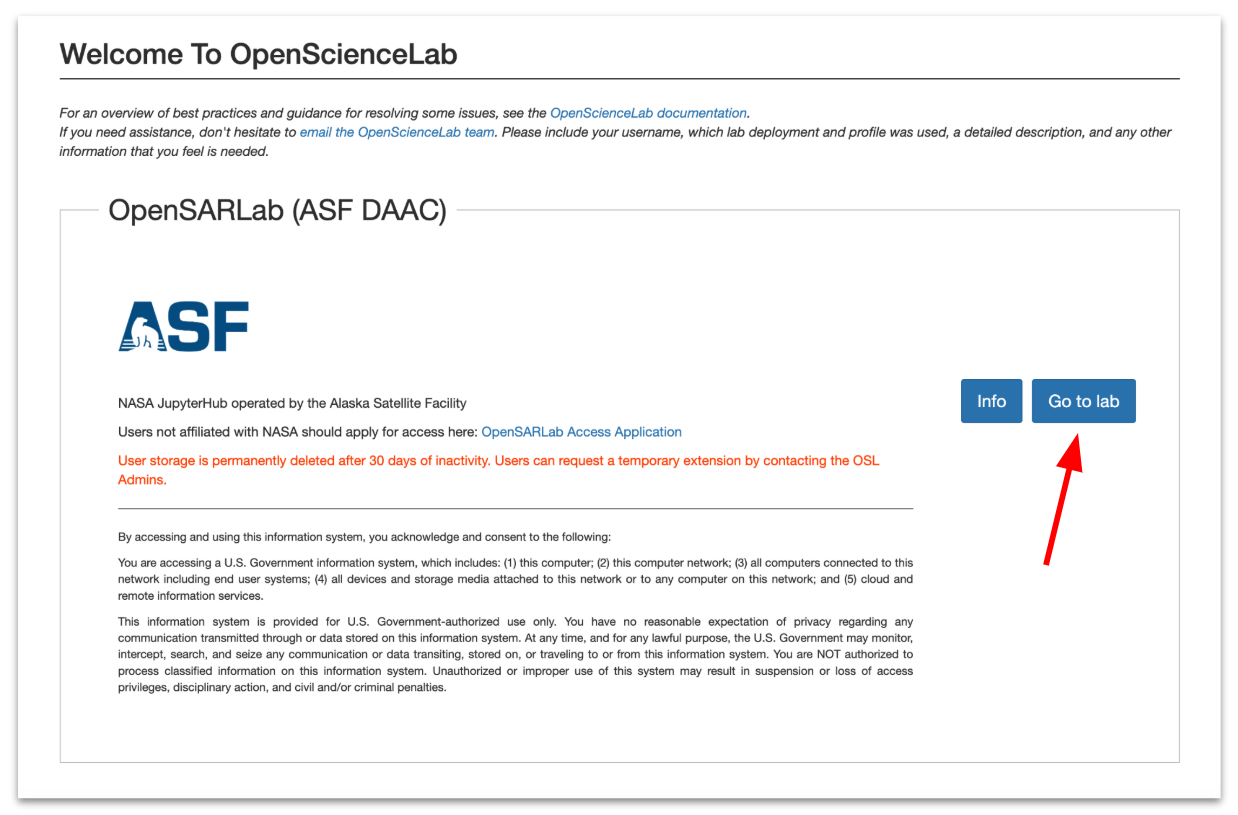
\includegraphics[width=0.7\linewidth]{files/opensciencelab_goto_-2d6003078519e1928c1d6adc33f7a29f.png}
\caption*{The OpenScienceLab Portal provides access to users' labs. In this example, there is only one lab available, but users will see lab cards for any labs to which they have access.}
\end{figure}

\begin{enumerate}[resume]
\item Click the \texttt{Start My Server} button.
\end{enumerate}

\begin{figure}[!htbp]
\centering
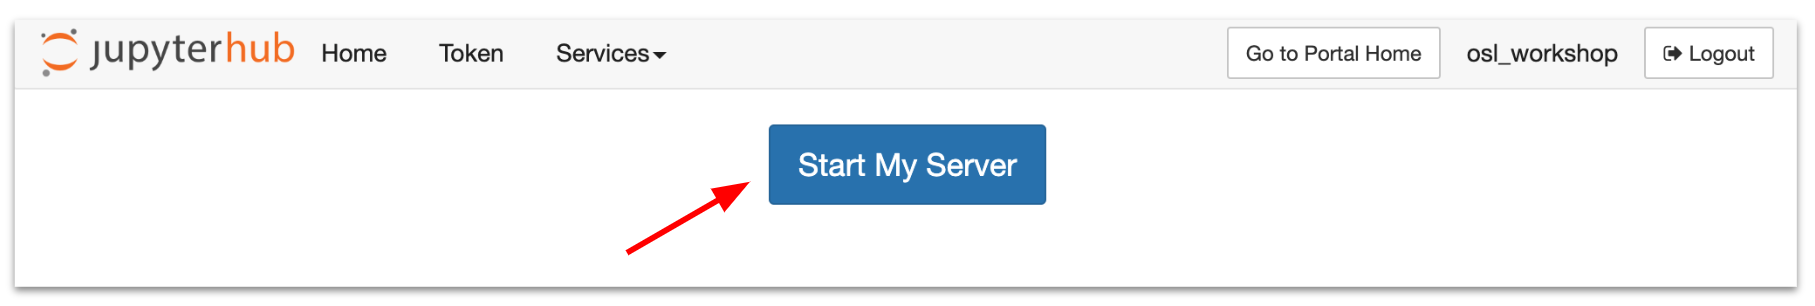
\includegraphics[width=0.7\linewidth]{files/start_server-f7c4d33c0700583fa6071e15002d6364.png}
\end{figure}

\begin{enumerate}[resume]
\item On the Server Options page, select the radio button of the server profile you wish to use and click the \texttt{Start} button.
\end{enumerate}

\begin{figure}[!htbp]
\centering
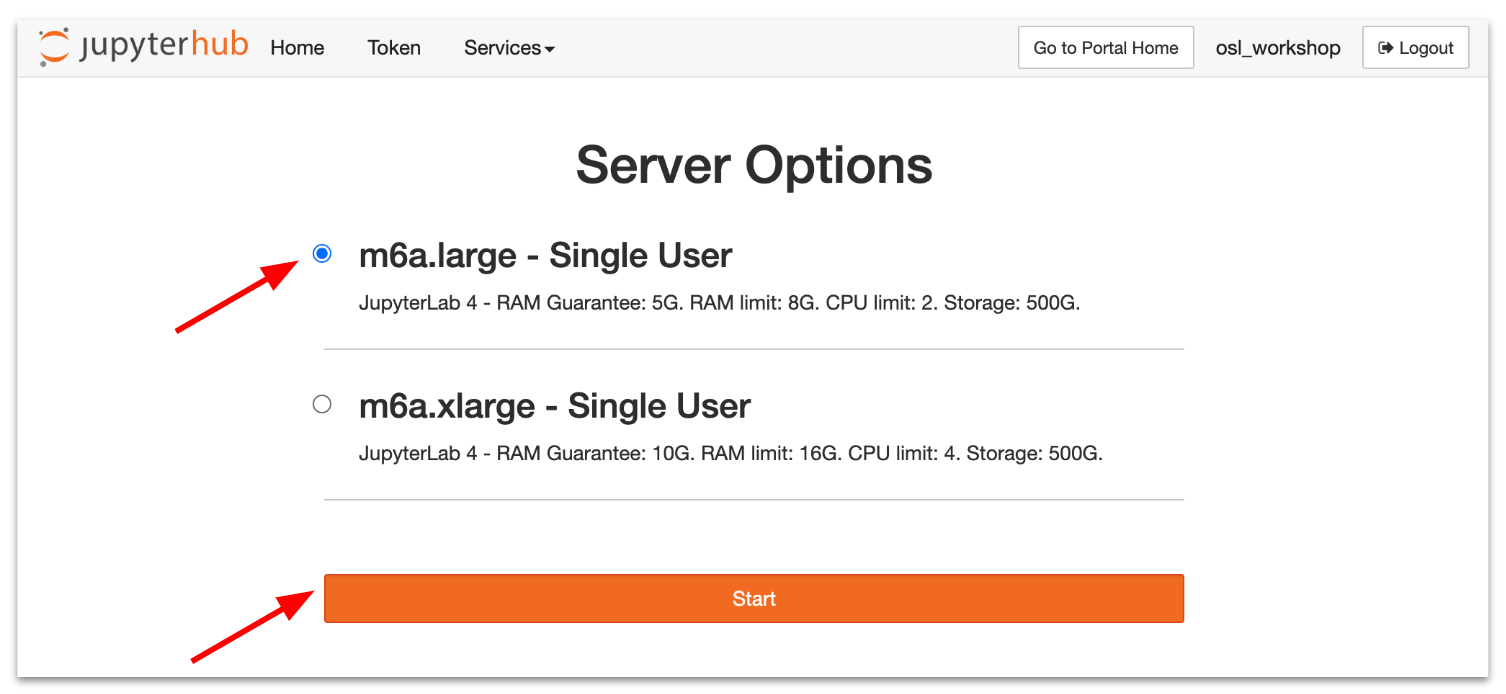
\includegraphics[width=0.7\linewidth]{files/server_profile_selec-04f0a0fc0dc0d4a8fa77778ddb497242.png}
\end{figure}

\begin{enumerate}[resume]
\item A status screen will load while your server starts.
\end{enumerate}

\begin{figure}[!htbp]
\centering
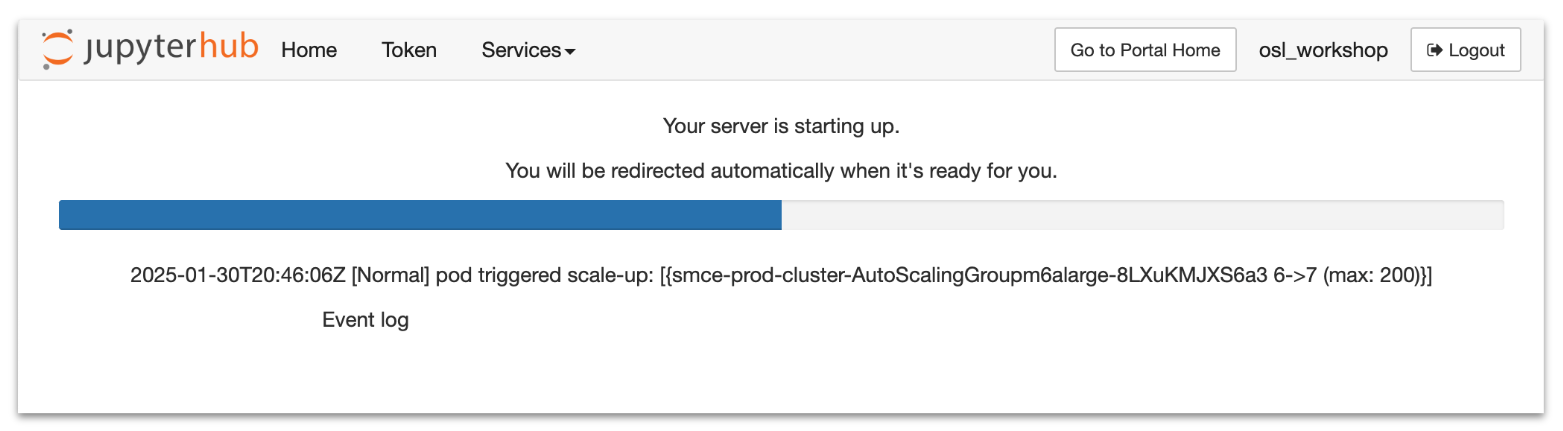
\includegraphics[width=0.7\linewidth]{files/server_status-bb8534988e98d7d4886c1eb6e2a8a7b1.png}
\end{figure}

\begin{enumerate}[resume]
\item You can click on ``Event Log'' to display the system logs as your server starts.
\end{enumerate}

\begin{figure}[!htbp]
\centering
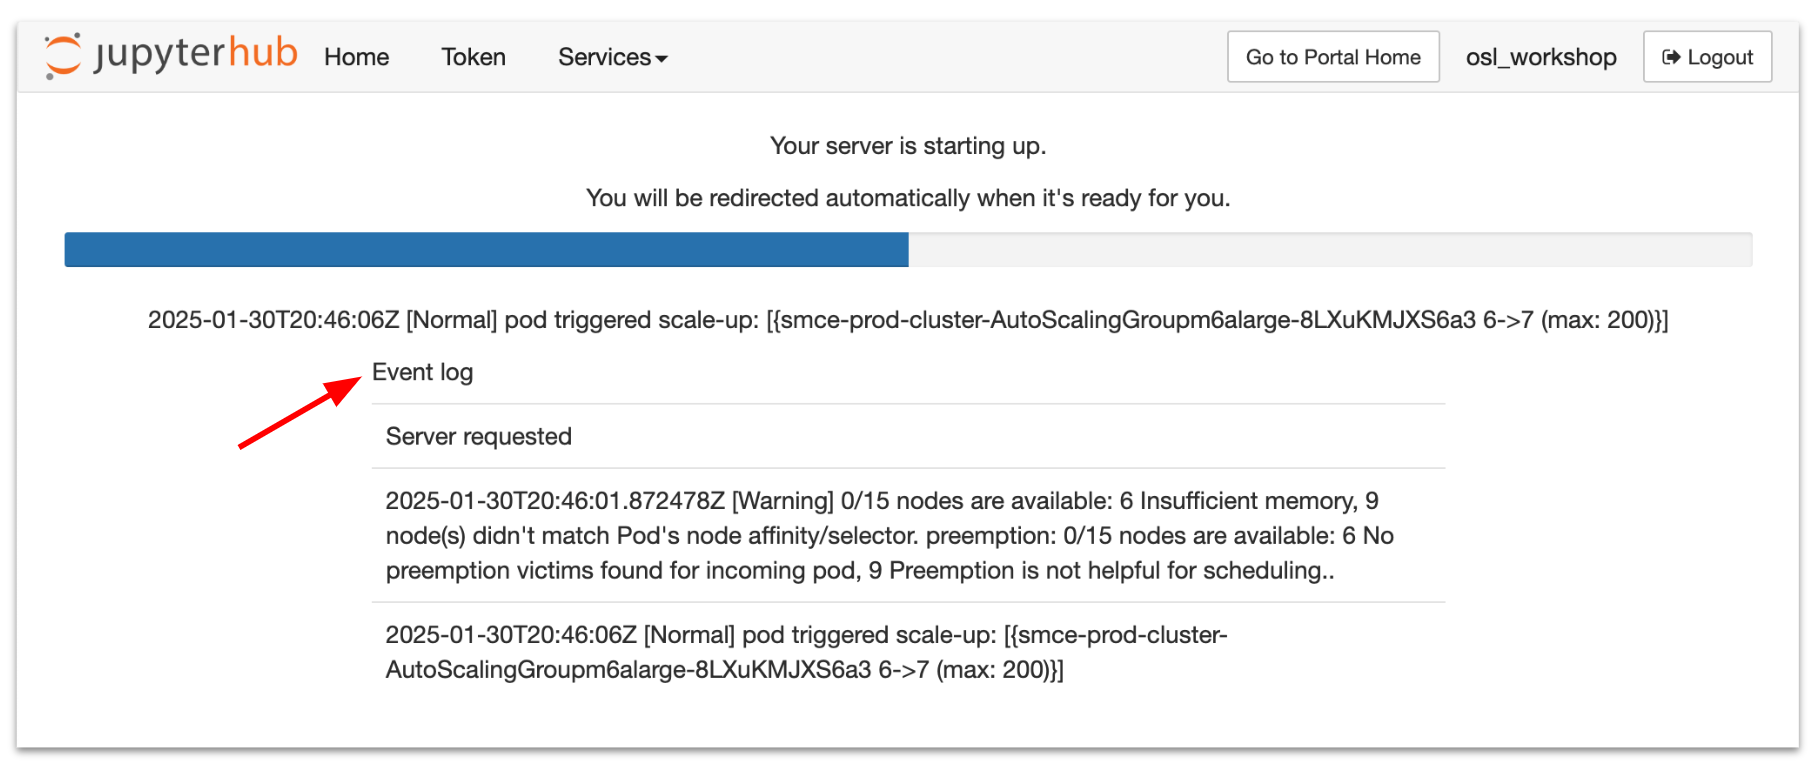
\includegraphics[width=0.7\linewidth]{files/event_log-a9d01375ba0ea46bdf88451ef1e3ecd3.png}
\end{figure}

\begin{enumerate}[resume]
\item It may take several minutes for a server to start. When it has started, you will have access to a JupyterLab desktop.
\end{enumerate}

\begin{figure}[!htbp]
\centering
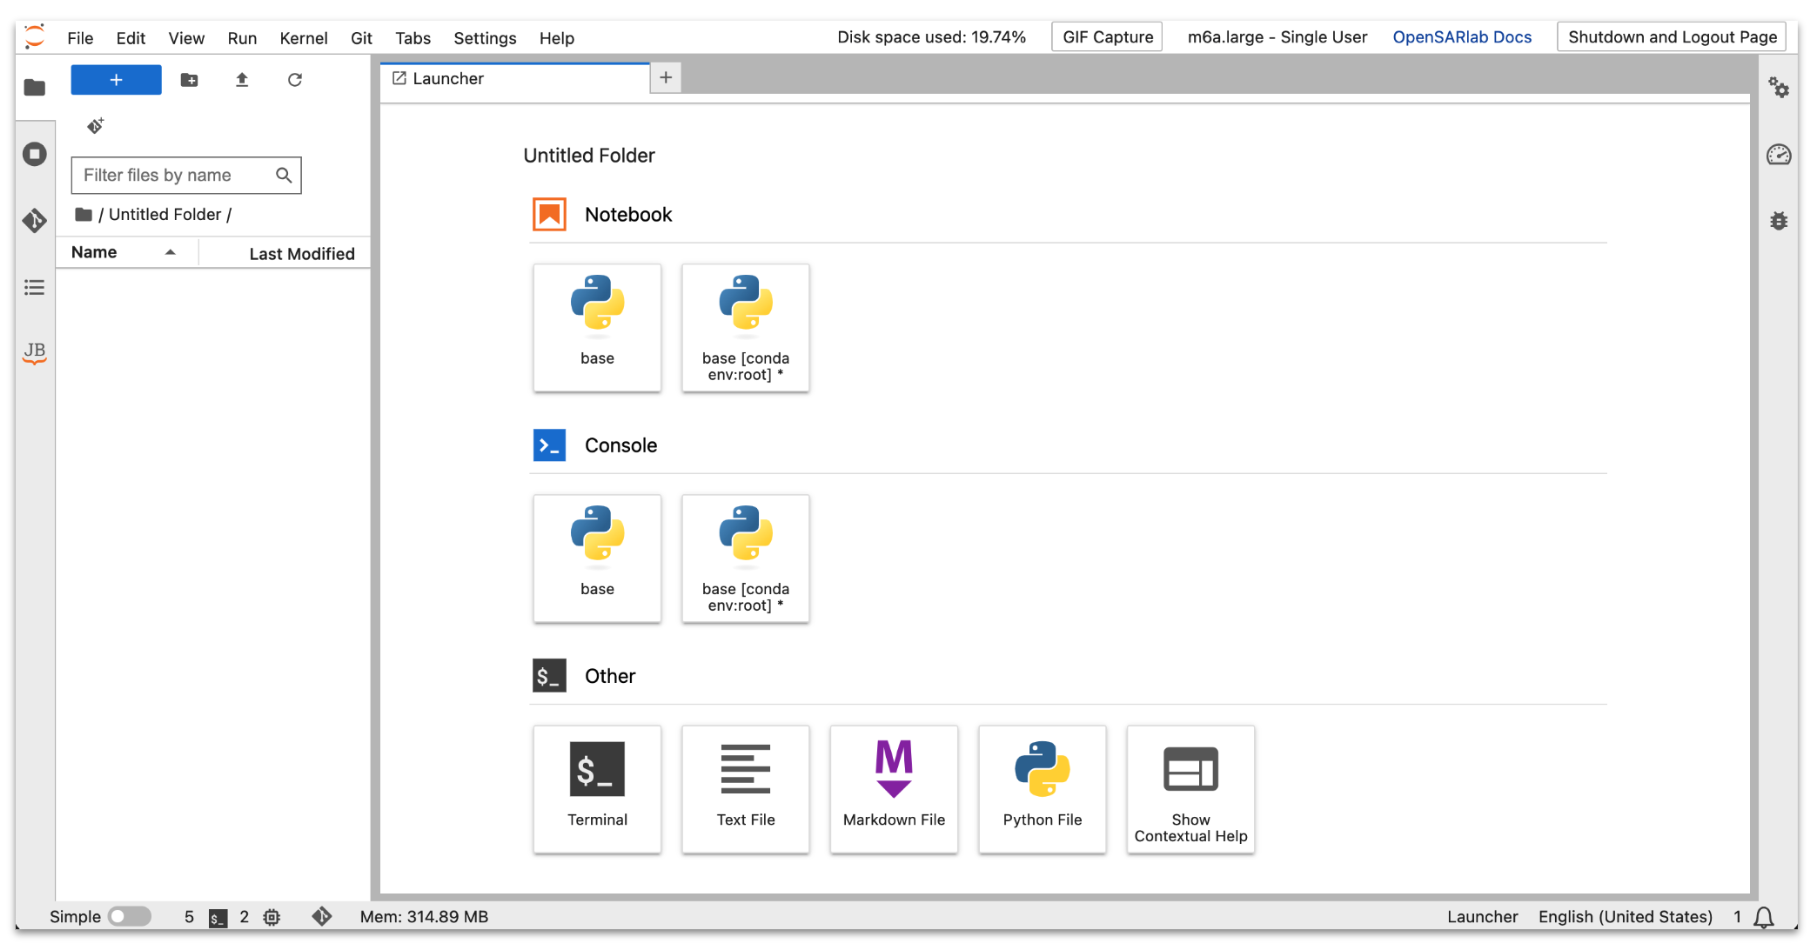
\includegraphics[width=0.7\linewidth]{files/jupyter_lab-fdc94447b7e46a4e672337bf84e8cf49.png}
\caption*{The JupyterLab desktop loads when your server has started. Depending on the specific lab, you may have access to varying notebook kernels and JupyterLab extensions.}
\end{figure}

\subparagraph{Stopping a Server}

\begin{enumerate}
\item Select \texttt{Hub Control Panel} from the \texttt{File} menu
\end{enumerate}

\begin{figure}[!htbp]
\centering
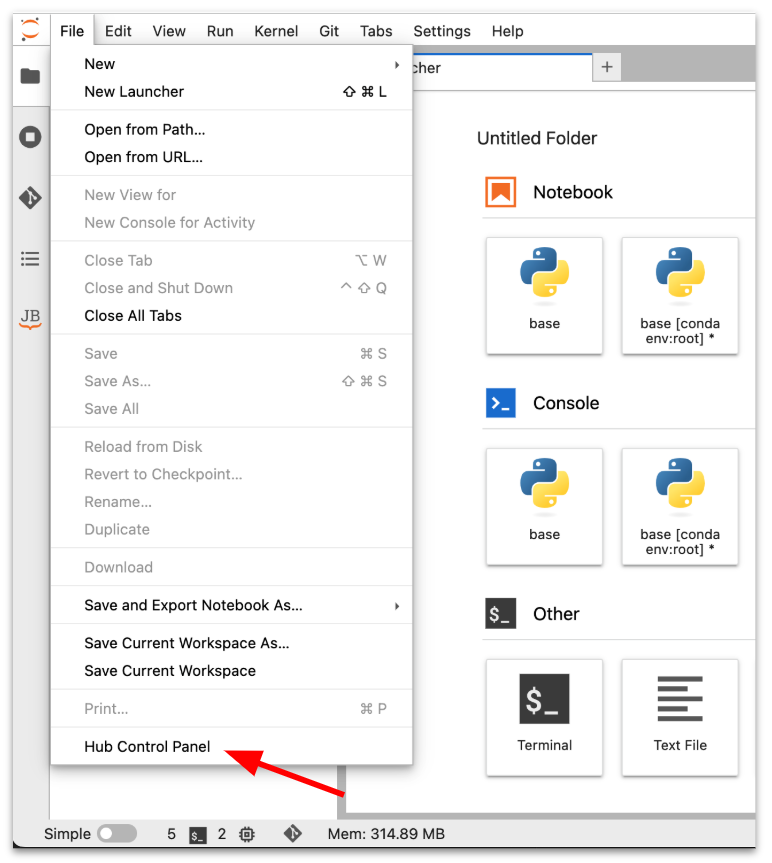
\includegraphics[width=0.7\linewidth]{files/jupyterhub_control_p-8d395ee205601c03418bf1a9e775c2d4.png}
\end{figure}

or

Click the \texttt{Shutdown and Logout Page} button at the top right of the JupyterLab desktop

\begin{figure}[!htbp]
\centering
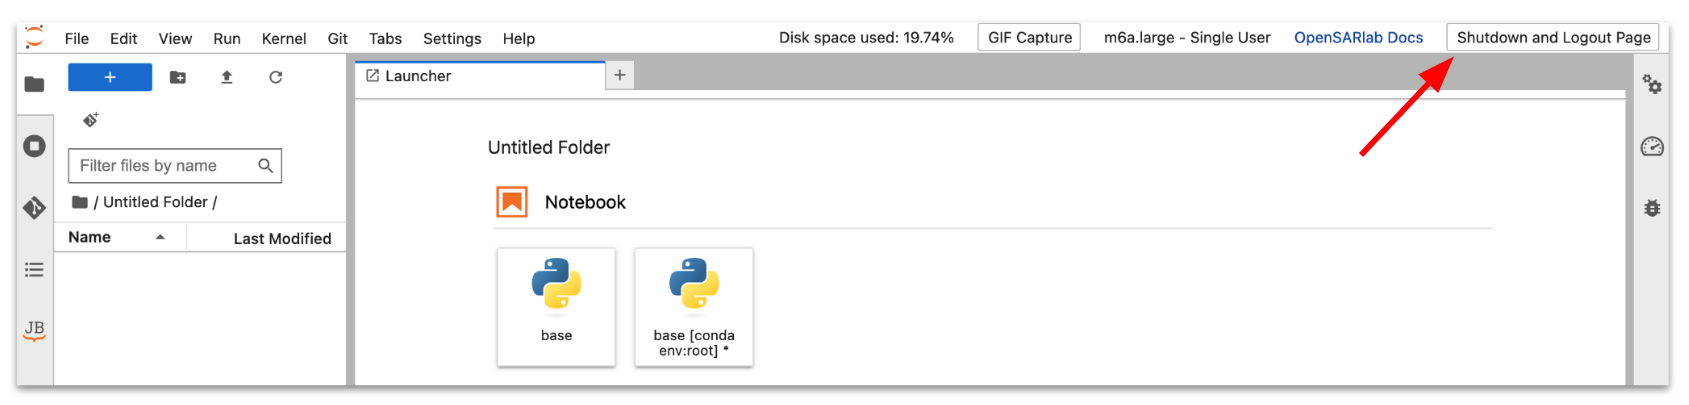
\includegraphics[width=0.7\linewidth]{files/shutdown_logout_butt-ebf28f7358ab734375ae40c2ef0d02e8.png}
\end{figure}

\begin{enumerate}[resume]
\item Click the \texttt{Stop My Server} Button
\end{enumerate}

\begin{figure}[!htbp]
\centering
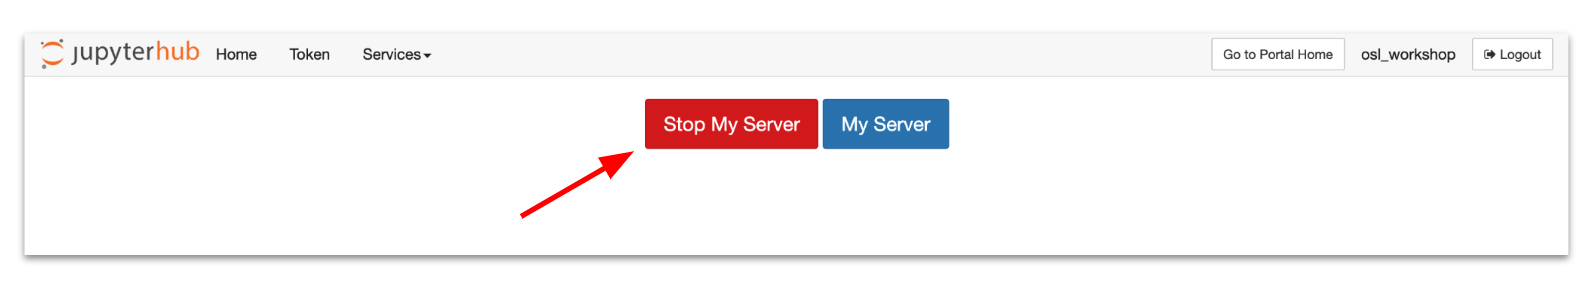
\includegraphics[width=0.7\linewidth]{files/stop_my_server-e8375d436e19a65eefdcf23fe9079287.png}
\end{figure}

\subsubsection{Jupyter Notebook Kernels}

\newline
Notebooks in OpenScienceLab run Python kernels corresponding to a variety of \href{https://docs.conda.io/en/latest/}{conda} software environments. Since notebooks have different software dependencies, it is important to run them in an appropriate kernel.

Each ASF-developed Jupyter Book of data recipes includes a notebook that creates the required conda environment.

At this time, we still have some Jupyter Notebooks that have not yet been organized into Jupyter Books. Each of these notebooks is pre-configured to use its required kernel. See our \href{./conda\_environments.md}{Conda environments documentation} for instructions on building those software environments.

\begin{itemize}
\item How~to~Switch~Notebook~Kernels
\item Restarting~a~Jupyter~Notebook~Kernel
\end{itemize}


\bigskip
\centerline{\rule{13cm}{0.4pt}}
\bigskip

\paragraph{How to Switch Notebook Kernels}\label{How-to-Switch-Notebook-Kernels}

\begin{enumerate}
\item Click the current kernel name in the upper right corner of a notebook.
\item A window with a list of available kernels will appear.
\item Select a \texttt{kernel}.
\end{enumerate}

\begin{figure}[!htbp]
\centering
\includegraphics[width=0.7\linewidth]{files/select_kernel-18aa49c1e61fd3c105a0c18bf3cb2706.gif}
\caption*{Changing a notebook's kernel.}
\end{figure}

\begin{framed}
\textbf{Are you missing a required kernel?}\\
You need to build its Conda environment. Instructions are provided \href{./conda\_environments.md}{here}.
\end{framed}


\bigskip
\centerline{\rule{13cm}{0.4pt}}
\bigskip

\paragraph{Restarting a Jupyter Notebook Kernel}\label{Restarting-a-Jupyter-Notebook-Kernel}

\begin{enumerate}
\item Click in the notebook tab to select it.
\item Select one of the following from the \texttt{Kernel} Menu:
\end{enumerate}

\begin{itemize}
\item \texttt{Restart Kernel}: Restarts the kernel but leaves any old code cell output in place.
\item \textbf{(Recommended)}\texttt{Restart Kernel and Clear All Outputs...}: Restarts the kernel and removes old code cell output.
\item \texttt{Restart Kernel and Run up to Selected Cell...}: Restarts the kernel and run up to the cell where you selected.
\item \texttt{Restart Kernel and Run All Cells...}: Restarts the kernel and runs all the code cells. \textbf{This only works with notebooks that do not require user input.}
\end{itemize}

\begin{framed}
\textbf{Restart the kernel before rerunning a notebook.}\\
While the ability to rerun the code cells in arbitrary order can be helpful, it can also cause problems, such as:

\begin{itemize}
\item Recycled variables may contain unexpected values if you run cells in non-sequential order.
\item You may skip cells that set required variables or perform necessary functions.
\item If you change directories in a code cell and run other cells in an unexpected order, you could attempt to run code in the wrong location.
\end{itemize}
\end{framed}

\subsubsection{Jupyter Terminal}

\paragraph{Overview}


\bigskip
\centerline{\rule{13cm}{0.4pt}}
\bigskip

JupyterLab provides an an interactive shell in a terminal.

\begin{framed}
\textbf{Use the terminal to easily delete non-empty directories}\\
Jupyter intentionally prevents the deletion of non-empty directories from the file browser. However, you can delete full directories from the command line in a terminal.

\texttt{rm -rf path/to/my/full/directory}
\end{framed}

\paragraph{\textbf{How to Open a Terminal}}


\bigskip
\centerline{\rule{13cm}{0.4pt}}
\bigskip

\begin{enumerate}
\item If there is no \texttt{Launcher} tab in your workspace, open one by clicking the blue \texttt{+} button at the upper left of the screen.
\end{enumerate}

\begin{figure}[!htbp]
\centering
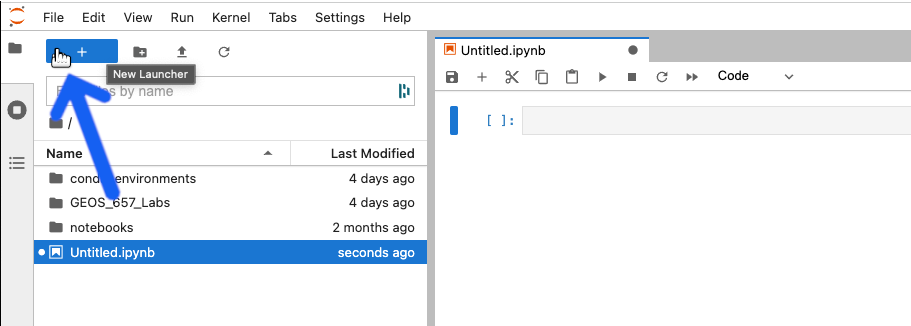
\includegraphics[width=0.7\linewidth]{files/launcher-c8502ccf02f11470216a123405d1af64.png}
\caption*{The JupyterLab \texttt{New Launcher} button}
\end{figure}

\begin{enumerate}[resume]
\item Click the \texttt{Terminal} button in the \texttt{Launcher} tab.
\end{enumerate}

\begin{figure}[!htbp]
\centering
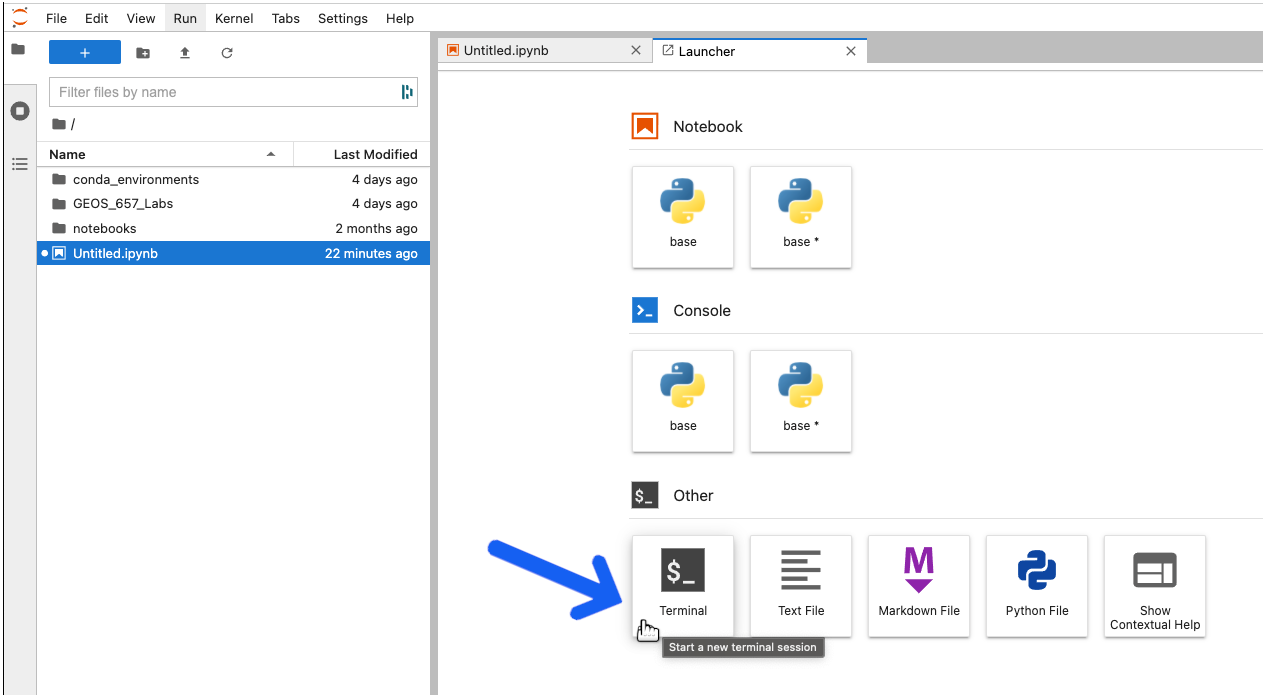
\includegraphics[width=0.7\linewidth]{files/jlab_terminal-f2d777f76897cfe77aa7041fd71d98ce.png}
\caption*{The JupyterLab \texttt{Terminal} button.}
\end{figure}

\begin{enumerate}[resume]
\item Use the terminal as you typically would.
\end{enumerate}

\begin{figure}[!htbp]
\centering
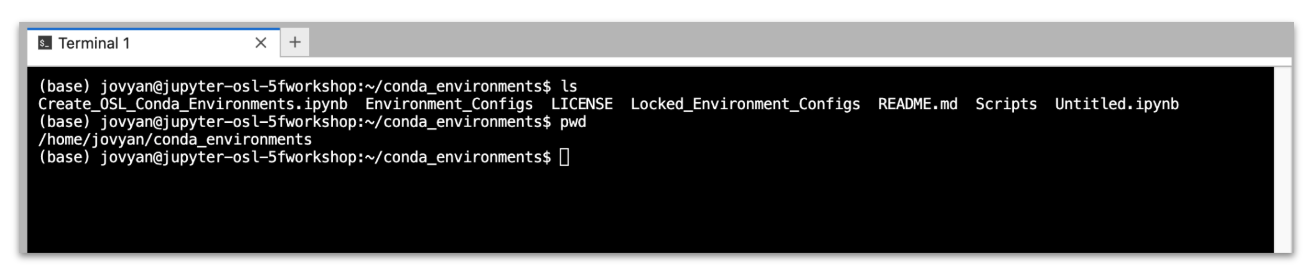
\includegraphics[width=0.7\linewidth]{files/terminal-9cc223d82afb11b942d56e6310abad5a.png}
\end{figure}


\bigskip
\centerline{\rule{13cm}{0.4pt}}
\bigskip

\begin{framed}
\textbf{No Root Privileges}\\
For security, OSL users do not have root privileges.

\begin{figure}[!htbp]
\centering
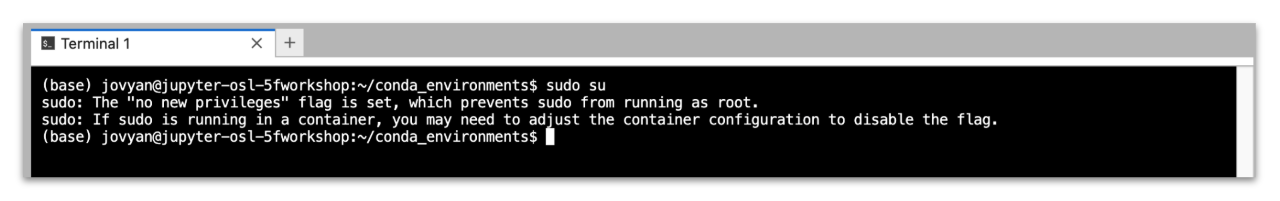
\includegraphics[width=0.7\linewidth]{files/no_sudo-d355e5fa49ab50be6c8011cc5806454e.png}
\end{figure}
\end{framed}

\subsubsection{Server Logout/Shutdown Best Practices}

\newline
Please shutdown your server after each work session to help reduce cloud costs.

\begin{framed}
\textbf{Logging out of OpenScienceLab does not shutdown your lab servers.}\\
While it is wise to logout of your account for reasons related to security, it will not stop any lab servers you may have left running. They will continue to run in the background, accruing costs. Please shutdown all running servers before logging out.
\end{framed}

\begin{itemize}
\item Why~Shut~Down~the~Server?
\item How~to~Shut~Down~The~Server~and~Logout~in~Jupyter~Lab
\item How~to~Log~Out~of~OpenScienceLab
\end{itemize}


\bigskip
\centerline{\rule{13cm}{0.4pt}}
\bigskip

\paragraph{Why Shut Down the Server?}\label{Why-Shut-Down-the-Server}

Cloud computing is expensive.

Please help us keep OpenSARLab available to as many users as possible and reduce costs for custom lab owners by shutting down servers when they are not in use.

\textbf{In some instances, you may need to leave your server running. For example, you
have a notebook performing a very time intensive analysis and wish to let it run
overnight. It is acceptable for you to keep your server running in cases like this.}


\bigskip
\centerline{\rule{13cm}{0.4pt}}
\bigskip

\paragraph{How to Shut Down The Server and Logout in Jupyter Lab}\label{How-to-Shut-Down-The-Server-and-Logout-in-Jupyter-Lab}

See the \href{/jupyter-servers}{Jupyter Server Documentation}


\bigskip
\centerline{\rule{13cm}{0.4pt}}
\bigskip

\paragraph{How to Log Out of OpenScienceLab}\label{How-to-Log-Out-of-OpenScienceLab}

\begin{enumerate}
\item Select \texttt{Hub Control Panel} from the \texttt{File} menu.
\end{enumerate}

\begin{figure}[!htbp]
\centering
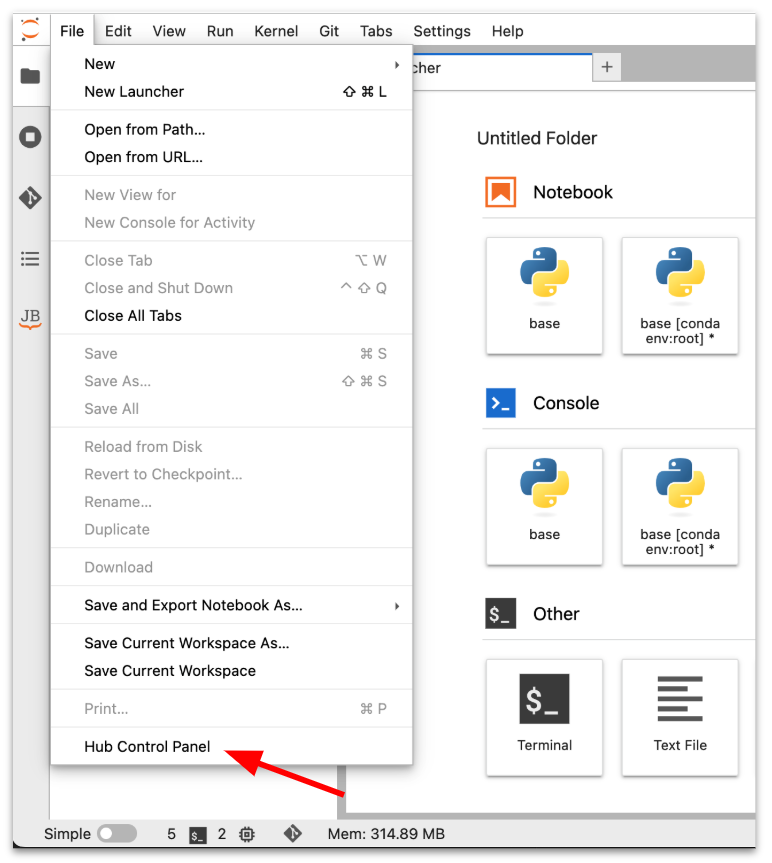
\includegraphics[width=0.7\linewidth]{files/jupyterhub_control_p-8d395ee205601c03418bf1a9e775c2d4.png}
\end{figure}

or

Click the \texttt{Shutdown and Logout Page} button at the top right of the JupyterLab desktop.

\begin{figure}[!htbp]
\centering
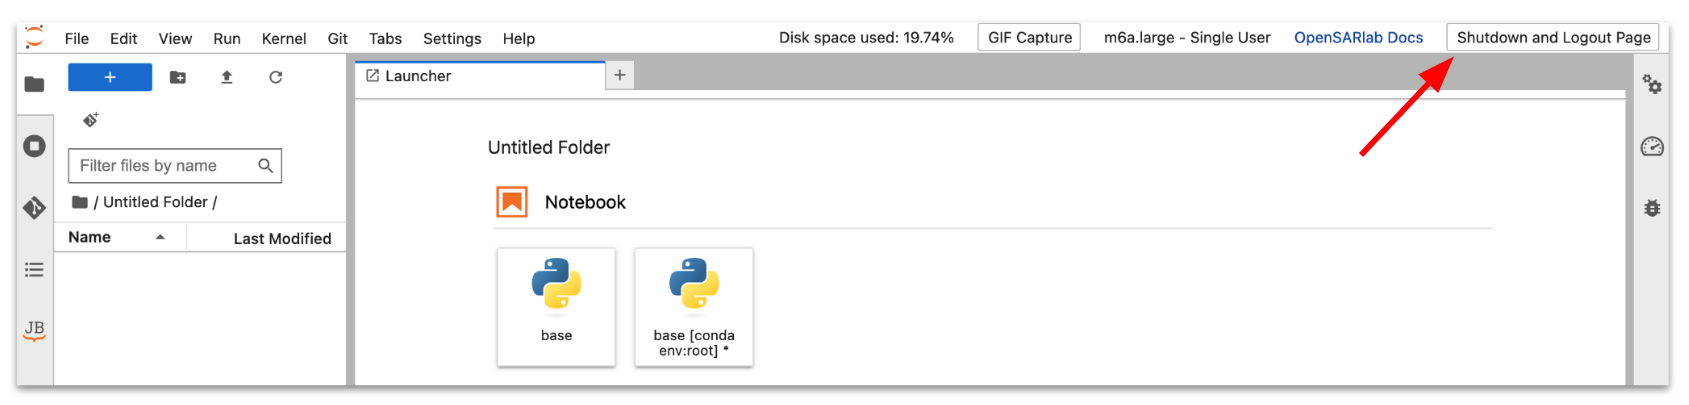
\includegraphics[width=0.7\linewidth]{files/shutdown_logout_butt-ebf28f7358ab734375ae40c2ef0d02e8.png}
\end{figure}

\begin{enumerate}[resume]
\item Click the \texttt{Logout} button.
\end{enumerate}

\begin{figure}[!htbp]
\centering
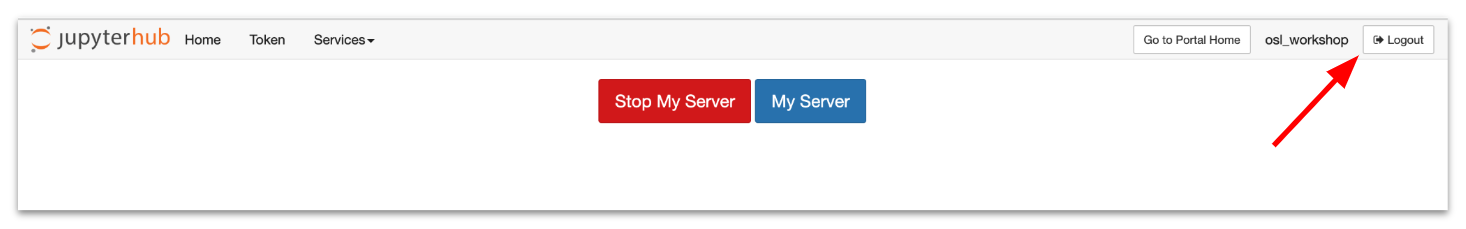
\includegraphics[width=0.7\linewidth]{files/logout-7fe193ded08c3eda77e9ad3f8bf6ea19.png}
\end{figure}

\subsubsection{JupyterLab Extensions}

\newline
As an OpenScienceLab user, you have limited access to third-party extensions.

\begin{itemize}
\item Server extensions must be installed in the OpenSARLab Docker container and cannot be installed by users.
\item Lab extensions can be installed, enabled, and disabled from the terminal but they will not persist across server restarts and will need to be reinstalled.
\end{itemize}

\begin{framed}
\textbf{Request an extension}\\
If you feel that OpenSARLab is lacking an important Jupyter Lab extension, please contact us to request it at \href{mailto:uaf-jupyterhub-asf@alaska.edu}{uaf-jupyterhub-asf@alaska.edu}

If you would like an extension added to a custom lab, we will need approval from the lab owner before installing it.
\end{framed}

\subsection{Installing Software in a Lab}

\begin{itemize}
\item Conda~Environments\begin{itemize}
\item Use~an~ASF-provided~notebook~and~environment.yml~to~create~a~Conda~environment
\item Install~Conda~packages~within~a~running~notebook’s~environment
\item Install~Conda~packages~in~an~existing~environment~from~the~terminal
\end{itemize}


\item pip\begin{itemize}
\item Install~pip~packages~inside~of~a~Conda~environment~from~the~terminal
\item Include~pip~packages~in~a~Conda~environment.yml
\end{itemize}


\item apt~and~apt-get
\end{itemize}


\bigskip
\centerline{\rule{13cm}{0.4pt}}
\bigskip

\subsubsection{Conda Environments}\label{Conda-Environments}

Users can install additional software in isolated Conda environments on their persistent storage volumes with \href{https://conda.io/projects/conda/en/latest/index.html}{conda} or \href{https://github.com/mamba-org/mamba}{mamba} (conda's faster reimplementation).

OpenSARLab user images include a default \texttt{base} conda environment with a minimal amount of software installed. Users may create additional conda environments on their persistent user volumes to support workflows in Jupyter Notebooks or Python scripts.

\begin{framed}
\textbf{ASF-provided Conda Environments}\\
The following conda environment config files are provided by ASF:

\begin{itemize}
\item \texttt{ARIA-tools}
\item \texttt{autorift}
\item \texttt{earthscope\_insar}
\item \texttt{isce3\_rtc}
\item \texttt{machine learning}
\item \texttt{rtc\_analysis}
\item \texttt{minimal\_notebook}
\item \texttt{nisar\_se}
\end{itemize}

These environments are not pre-built; users must create their conda environments and register their kernels with \texttt{ipykernel} to make them accessible in notebooks. We provide a notebook to help install conda environments and register their kernels. \textbf{This can be done from the terminal if you are comfortable with Conda} or you can use an ASF-provided notebook to walk through the process.
\end{framed}

\paragraph{Use an ASF-provided notebook and \texttt{environment.yml} to create a Conda environment}\label{Use-an-ASF-provided-notebook-and-environment-yml-to-create-a-Conda-environment}

\begin{enumerate}
\item Open the following notebook: \href{https://opensciencelab.asf.alaska.edu/lab/smce-prod-opensarlab/hub/user-redirect/lab/tree/conda\_environments/Create\_OSL\_Conda\_Environments.ipynb}{\texttt{/home/jovyan/conda\_environments/Create\_OSL\_Conda\_Environments.ipynb}}
\item Run the notebook to select and build one of the available environments.\begin{itemize}
\item Alternatively, the notebook allows you to point to a custom \texttt{environment.yml} that you provide.
\end{itemize}
\end{enumerate}

\begin{framed}
\textbf{Note}\\
\begin{itemize}
\item Once an environment is created and its kernel is registered, it may take another couple of minutes for Jupyter to recognize it and display it as an available kernel option.
\item ASF has started migrating data recipes into Jupyter Books, which are organized collections of Jupyter Notebooks with an interactive table of contents. Each Jupyter Book includes a notebook to build any required conda environments. This can be run directly from the Jupyter Book, in which case there is no need to build an environment using the \texttt{/home/jovyan/conda\_environments/Create\_OSL\_Conda\_Environments.ipynb} described above.
\end{itemize}
\end{framed}

\paragraph{Install Conda packages within a running notebook's environment}\label{Install-Conda-packages-within-a-running-notebooks-environment}

\begin{enumerate}
\item Run the following command in a code cell:
\end{enumerate}

\begin{verbatim}
%mamba install -c conda -forge <package_name> - -yes
\end{verbatim}

\paragraph{Install Conda packages in an existing environment from the terminal}\label{Install-Conda-packages-in-an-existing-environment-from-the-terminal}

\begin{enumerate}
\item Open a terminal and run the following commands:
\end{enumerate}

\begin{verbatim}
mamba activate <environment_name>
mamba install <package_name>
\end{verbatim}

\begin{framed}
\textbf{Avoid installing software in the \texttt{base} Conda environment}\\
Packages installed in the \href{https://conda.io/projects/conda/en/latest/user-guide/getting-started.html\#managing-envs}{base conda environment} will not persist after an OpenScienceLab server shuts down. The \texttt{base} environment is located in a Docker container that will be replaced with a container using a freshly pulled copy of its image on server startup.

We recommend installing Conda packages in non-base environments rather than in \texttt{base}. These environments are stored in the \texttt{{\textasciitilde}/.local/env} directory on persistent storage volumes and they will remain after the server restarts.
\end{framed}


\bigskip
\centerline{\rule{13cm}{0.4pt}}
\bigskip

\subsubsection{pip}\label{pip}

\href{https://pip.pypa.io/en/stable/}{\textit{pip}} is a package installer for Python.

You can install \texttt{pip} packages onto your persistent volume in the following manner:

\paragraph{Install \texttt{pip} packages inside of a Conda environment from the terminal}\label{install-pip-packages-inside-of-a-Conda-environment-from-the-terminal}

\begin{enumerate}
\item Open a terminal and use the following commands:
\end{enumerate}

\begin{verbatim}
conda activate <environment_name>
python -m pip install <package_name>
\end{verbatim}

\paragraph{Include pip packages in a Conda \texttt{environment.yml}}\label{Include-pip-packages-in-a-Conda-environment-yml}

\begin{enumerate}
\item Include \texttt{pip} in the dependency list
\item Add a \texttt{pip} section to the bottom of the dependency list in an \texttt{environment.yaml}
\end{enumerate}

\begin{verbatim}
name: environment name
channels:
  - conda -forge
dependencies:
  - package_1
  - package_2
  - package_3
  - pip
  - pip:
    - pip_package_1
    - pip_package_2
\end{verbatim}

\begin{framed}
\textbf{We recommend against pip installations with the \texttt{--user} argument in OpenSARLab}\\
This will install the package in your \texttt{/home/jovyan/.local/lib/python3.x/site-packages} directory and will supersede any installations of the same package in a Conda environment. This can cause issues and confusion when a user installs a specific required package version in a Conda environment, but a previously installed version in an unexpected location is used instead.
\end{framed}


\bigskip
\centerline{\rule{13cm}{0.4pt}}
\bigskip

\subsubsection{apt and apt-get}\label{apt-and-apt-get}

Users cannot install software in OpenScienceLab using \texttt{apt} or \texttt{apt-get}.

\subsection{Storage and Source Control (Git)}

\begin{itemize}
\item \href{/opensciencelab-storage}{Storage in OpenScienceLab}
\item \href{/s3-buckets}{Accessing S3 Buckets}
\item \href{/git-in-opensarlab}{Git}
\end{itemize}

\subsubsection{Storage in OpenScienceLab}

\newline
In OpenScienceLab, users have access to both ephemeral and persistent storage.

\paragraph{Ephemeral Storage}

OpenScienceLab servers run in a \href{https://www.docker.com/resources/what-container/}{Docker container} that uses a pre-built \href{https://docs.docker.com/get-started/docker-concepts/the-basics/what-is-an-image/}{Docker image}. Each user container comes with ephemeral storage containing the user's root directory.

Much of this ephemeral storage is locked down, and users cannot write to it.

\begin{framed}
\textbf{Warning}\\
Nothing written to directories above the user \texttt{home} directory (\texttt{/home/jovyan}) will persist across server restarts.
\end{framed}


\bigskip
\centerline{\rule{13cm}{0.4pt}}
\bigskip

\paragraph{Persistent Storage}

OpenScienceLab users typically have access to persistent storage in all their labs, but individual lab owners determine this.

Assuming a lab has persistent storage, it occupies the user's \texttt{home} directory (\texttt{/home/jovyan}).

\begin{framed}
\textbf{Storage in OpenSARLab}\\
\begin{itemize}
\item OpenSARLab users have access to 500GB of persistent storage
\item Persistent storage is permanently deleted after 30 days of inactivity. Warning emails are sent to inactive users after 29, 27, and 24 days.
\end{itemize}
\end{framed}

\begin{framed}
\textbf{Keep track of available persistent storage space with the storage monitor}\\
\begin{figure}[!htbp]
\centering
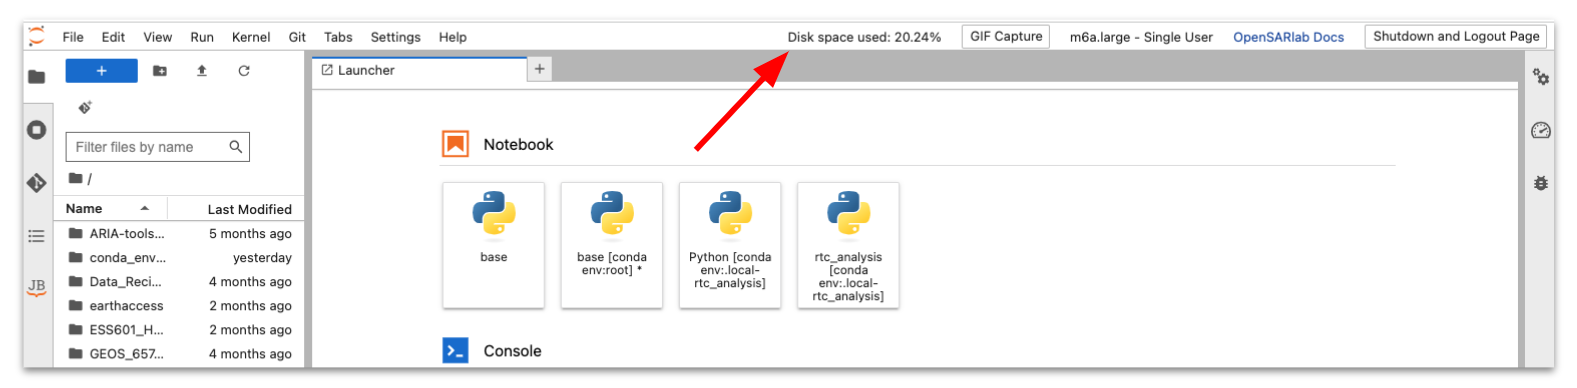
\includegraphics[width=0.7\linewidth]{files/storage_monitor-adefe078b91a683b2d14724e1b331377.png}
\end{figure}
\end{framed}

\subsubsection{Accessing S3 Buckets}

\newline
OpenScienceLab user servers typically run in AWS region \texttt{us-west-2}, which houses all public NASA data. This provides cheap, low-latency data access.

You may access any public AWS S3 bucket or private bucket to which you have permission with either the \texttt{aws-cli} (command line interface) or \texttt{boto3} (Python package).

\begin{framed}
\textbf{Configure the AWS Client in your OpenScienceLab account for non-public bucket access.}\\
\textit{Prerequisite: an AWS access key that provides access to the S3 bucket}

\begin{enumerate}
\item Open a terminal
\item Run the command: \texttt{aws configure}
\item When prompted, provide:\begin{itemize}
\item \texttt{AWS Access Key ID}
\item \texttt{AWS Secret Access Key}
\item \texttt{Default region name}: ``us-west-2''
\item \texttt{Default output format}: ``json''
\end{itemize}
\end{enumerate}
\end{framed}

\begin{framed}
\textbf{Warning}\\
If accessing a public S3 bucket anonymously, you must either:

\begin{itemize}
\item Provide the \texttt{--no-sign-request} argument to AWS-cli
or
\item Provide an \texttt{UNSIGNED} config to the boto3 S3 bucket resource:\begin{itemize}
\item \texttt{s3 = boto3.resource('s3', config=Config(signature\_version=UNSIGNED))}
\end{itemize}
\end{itemize}
\end{framed}

\paragraph{Example Notebook Demonstrating S3 Bucket Access with \texttt{AWS-cli} and \texttt{boto3}}

\href{https://github.com/ASFOpenSARlab/NISAR-Early-Adopters-Workshop-Oct-2024/blob/main/S3\_Buckets\_Upload\_Download.ipynb}{S3\_Buckets\_Upload\_Download.ipynb}

\begin{verbatim}

\end{verbatim}

\subsubsection{Git}

\paragraph{\textbf{Prerequisite}}


\bigskip
\centerline{\rule{13cm}{0.4pt}}
\bigskip

\begin{itemize}
\item \href{https://git-scm.com/about}{Git} - Version control systems that allow you to track changes to your files.
\item \href{https://github.com/asfadmin/asf-jupyter-notebooks}{ASF's Jupyter Notebook} - A collection of Jupyter Notebooks used in OpenSARLab.
\item \href{./OpenSARLab\_terminal.md}{Terminal} - A built-in terminal within OpenScienceLab. The user should also have a basic understanding of Bash commands.
\end{itemize}


\bigskip
\centerline{\rule{13cm}{0.4pt}}
\bigskip

\paragraph{\textbf{Gitpuller}}


\bigskip
\centerline{\rule{13cm}{0.4pt}}
\bigskip

A \href{https://jupyterhub.github.io/nbgitpuller/}{nbgitpuller} pulls any changes to the \href{https://github.com/ASFOpenSARlab/opensarlab-notebooks}{notebook repo} each time an OpenSARLab deployment server starts up.

In short words, \texttt{nbgitpuller} will automatically update the notebooks to the latest version.

If a user has made changes to a notebook and the same notebook has been updated by ASF in the \texttt{asf-jupyter-notebooks} repo, the following will occur:

Users will retain two copies of the same notebook.

\begin{itemize}
\item The user-edited notebook will have a timestamp appended to its name.
\item The notebook with the original name will contain the new changes made by ASF.
\end{itemize}

\textit{Example:}

\textit{Before Edit}

\begin{itemize}
\item Original version: \texttt{sample\_notebook.ipynb}
\end{itemize}

\textit{After Edit}

\begin{itemize}
\item Updated by user: \texttt{sample\_notebook\_\_20210616165846.ipynb}
\item Updated by ASF: \texttt{sample\_notebook.ipynb}
\end{itemize}

\textbf{NB: The \texttt{nbgitpuller} will only run if you are in the \texttt{main} branch of the \texttt{asf-jupyter-notebook} repo.}

%   So is this saying that if one file is missing from remote then none of the files from remote will be pulled? Thus removing one remote file will sabotage the whole thing?


\bigskip
\centerline{\rule{13cm}{0.4pt}}
\bigskip

\paragraph{\textbf{In the case of a broken Git state}}


\bigskip
\centerline{\rule{13cm}{0.4pt}}
\bigskip

Due to its complexity, it is common for users to break Git workflow. A broken Git state can lead to unexpected results, such as notebooks not being updated.

Below are the steps users can take if the Git workflow is in a state beyond their ability to repair.

\textit{Repair Process:}

\begin{enumerate}
\item Preserve any files/directories you wish to keep under the \texttt{/home/jovyan/notebooks} directory.\begin{itemize}
\item Either *\textit{download} or \textit{move out} items you wish to keep.
\end{itemize}


\item Delete the entire \texttt{/home/jovyan/notebooks} directory.\begin{itemize}
\item Use \texttt{rm -rf /home/jovyan/notebooks} on the terminal to delete all.
\end{itemize}


\item Restart your server.
\item Gitpuller will automatically clone a clean repository into your account.
\end{enumerate}

*\textbf{NB}: When downloading a directory, users may compress them first to optimize downloading. The below commands will allow users to (de)compress files/directories:

\begin{itemize}
\item Compress: \texttt{zip -r \textless name\textgreater .zip \textless directory\textgreater }
\item Decompress: \texttt{unzip \textless name\textgreater .zip}
\end{itemize}

Where \texttt{\textless name\textgreater } can be anything you wish.


\bigskip
\centerline{\rule{13cm}{0.4pt}}
\bigskip

\paragraph{\textbf{Using Other Git Repos in OpenScienceLab}}


\bigskip
\centerline{\rule{13cm}{0.4pt}}
\bigskip

If you wish to utilize repositories other than those hosted by ASF, you can clone them into your OpenScienceLab account. However, users will need to manage the repos that they clone to prevent any issues.

When cloning a repository from elsewhere, users must ensure not to nest git repositories, i.e., do not clone a repository within another repository.

To avoid complications, \textbf{clone your repos to \texttt{/home/jovyan}}.

\section{Developer Guide}

\include{book-about-opensciencelab}

\subsection{Build and Deploy: Portal}

\subsubsection{Enable Under Construction page}

Sometimes the Portal must be taken down for updates. For instance, the EC2 the Portal runs on needs to be respawned for updates.

To help facilitate communication with users, an Under Construction page can be enabled. All traffic to the Portal will be redirected to this page.

\begin{enumerate}
\item To enable the page, log into the AWS account and go to EC2 console.


\item Go to the Portal load balancer, select the \texttt{HTTPS:443} listener, and \textit{check} the Default rule.


\item In the dropdown Actions menu, select Edit Rule.


\item Set the instance target group weight to \textbf{0}. Set the lambda target group weight to \textbf{1}.


\item At the bottom of the page Save Changes.


\item Changes should take affect almost immediately.
\end{enumerate}

To revert changes after updating, repeat the above steps except change the target group weights so that the instance gets \textbf{1} and the lambda gets \textbf{0}.

\subsubsection{----------}

The following documentation is older and must be used with caution.

\subsubsection{Prerequisites}

\paragraph{AWS SES: Store SES secrets}

These secrets will be used to communicate with SES to send emails. ``SMTP credentials consist of a username and a password. When you click the Create button below, SMTP credentials will be generated for you.'' The credentials are AWS access keys, like as used in local aws configs. They are valid for the whole region. \href{https://us-west-2.console.aws.amazon.com/ses/home}{https://us-west-2.console.aws.amazon.com/ses/home}

\begin{itemize}
\item Create a verified email and take out of sandbox.


\item Create SES serets

Go to \texttt{Account Dashboard} \textgreater  \texttt{Create SMTP credentials}. The IAM User Name should be unique and easy to find within IAM. On user creation, SMTP credentials will be created.


\item Store SES secrets

\begin{enumerate}
\item Go to \href{https://us-west-2.console.aws.amazon.com/secretsmanager/home}{https://us-west-2.console.aws.amazon.com/secretsmanager/home}


\item Click on \texttt{Store New Secret} \textgreater  \texttt{Other type of secret} \textgreater  \texttt{Plaintext}


\item Delete all empty json content.


\item Add username and password as given previously in the following format: \texttt{USERNAME PASSWORD}.


\item Click \texttt{Next}


\item Secret Name: \texttt{portal/ses-creds}, Tags: \texttt{osl-billing: osl-portal}


\item Click \texttt{Next}


\item Click \texttt{Next}


\item Click \texttt{Store}
\end{enumerate}
\end{itemize}

\paragraph{AWS Secrets Manager: Create SSO token}

This token will be used by the labs to communicate and authenticate with the portal. All labs and the portal share this token. It is imperative that this remains secret. The form of the token is very specific. Use the following process to create the token.

\begin{itemize}
\item Create secret

\begin{verbatim}
pip install cryptography
\end{verbatim}

\begin{verbatim}
from cryptography.fernet import Fernet

api_token = Fernet.generate_key()
api_token
\end{verbatim}


\item Add to AWS Secret Manager

\begin{enumerate}
\item Go to \href{https://us-west-2.console.aws.amazon.com/secretsmanager/home}{https://us-west-2.console.aws.amazon.com/secretsmanager/home}


\item Click on \texttt{Store New Secret} \textgreater  \texttt{Other type of secret} \textgreater  \texttt{Plaintext}


\item Delete all empty json content.


\item Add \textit{api\_token}.


\item Click \texttt{Next}


\item Secret Name: \texttt{\$CONTAINER\_NAMESPACE/sso-token}, Tags: \texttt{osl-billing: osl-portal}


\item Click \texttt{Next}


\item Click \texttt{Next}


\item Click \texttt{Store}
\end{enumerate}
\end{itemize}

\paragraph{Docker registry}

For local dev development, one can use a local docker registry.
\texttt{docker run -d -p 5000:5000 --restart=always --name registry registry:2}

Otherwise, the remote docker images will be stored in AWS ECR, as setup by CloudFormation

\paragraph{Docker repo}

Clone the portal code: \texttt{git clone git@github.com:ASFOpenSARlab/deployment-opensciencelab-prod-portal.git}

\subsubsection{Setup}

If production, upload the Cloudformation template \texttt{cf-portal-setup.yaml} and build.

Once the cloudformation is done, go to EC2 Connect of the portal EC2, log onto the server and \texttt{cd /home/ec2-user/code}.
Then setup prerequisites via \texttt{make setup-ec2}.
Note that you will be warned about reformatting the DB volume. If this is the first time running (as it should be), do so.

If locally, go to the root of the docker repo.
Then setup prerequisites via \texttt{make setup-ubuntu}.

\subsubsection{Build}

\texttt{cp labs.example.yaml labs.\{maturity\}.yaml}. The name of the config doesn't matter (except it cannot be labs.run.yaml)
Update labs.\{maturity\}.yaml as needed

\texttt{make config=labs.\{maturity\}.yaml}

\subsubsection{Destroy}

If production, clear out the registry images, delete the CloudFormation setup, delete db ebs snapshots, and delete logs.

If locally, \texttt{make clean} and then stop the localhost registry (if being used).

\subsubsection{Other less used procedures}

\paragraph{Logs}

In production, normally the logs will show up in CloudWatch.

For both, \texttt{docker compose logs -f}.

\paragraph{Replace Portal DB from snapshot}

If the Portal DB needs to be replaced by a snapshot backup, do the following.

\textit{Unless otherwise sated, all of these steps take place within EC2 Connect.}

Elevated permissions will be needed via \texttt{sudo} or \texttt{sudo su -}.

\begin{enumerate}
\item Restore backup snapshot to volume

This procedure assumes that the usual DB volume is present and being used. We only want to update the DB file.

Within \texttt{cf-portal-setup.yaml}, it is assumed that the AZ of the EC2's subnet is set as us-west-2a.

a. From the EC2 console, select the snapshot that will be restored. Get the SNAPSHOT\_ID, e.g. snap-0c0dbee2e7c9f0c12

b. From the EC2 console, select the portal EC2. Get the EC2\_INSTANCE\_ID, e.g. i-0ca96843e97d9bd29

c. First run a dry run to make sure permissions are available for EBS volume creation.
\texttt{     aws ec2 create-volume {\textbackslash}~         --dry-run {\textbackslash}~         --availability-zone us-west-2a {\textbackslash}~         --snapshot-id \$SNAPSHOT\_ID {\textbackslash}~         --tag-specifications 'ResourceType=volume,Tags=[\{Key=Name,Value=portal-db-backup\}]'     }

\begin{verbatim}
Then actually create an EBS volume from the backup snapshot.
 ```
 aws ec2 create -volume \
     - -availability -zone us -west -2a \
     - -snapshot -id $SNAPSHOT_ID \
     - -tag -specifications 'ResourceType=volume,Tags=[{Key=Name,Value=portal -db -backup}]'
 ```

 From response output, get VOLUME_ID, e.g. vol -0a0869b5ab9f77090
\end{verbatim}


\item Attach backup volume to EC2

First run a dry run to make sure permissions are available.

\begin{verbatim}
aws ec2 attach -volume \
    - -dry -run \
    - -device /dev/sdm \
    - -instance -id $EC2_INSTANCE_ID \
    - -volume -id $VOLUME_ID
\end{verbatim}

Then actually run it.

\begin{verbatim}
aws ec2 attach -volume \
    - -device /dev/sdm \
    - -instance -id $EC2_INSTANCE_ID \
    - -volume -id $VOLUME_ID
\end{verbatim}


\item Mount device to filesystem

\texttt{sudo mkdir -p /tmp/portal-db-from-snapshot/}
\texttt{sudo mount /dev/sdm /tmp/portal-db-from-snapshot/}

If you get an error message something like

\begin{quote}
/wrong fs type, bad option, bad superblock
\end{quote}

then you cannot mount the filesystem. AWS's way of handling volumes makes things difficult. \href{https://serverfault.com/questions/948408/mount-wrong-fs-type-bad-option-bad-superblock-on-dev-xvdf1-missing-codepage}{https://serverfault.com/questions/948408/mount-wrong-fs-type-bad-option-bad-superblock-on-dev-xvdf1-missing-codepage}

Since we are working with a temporay mount, run the following instead:

\texttt{sudo mount -t xfs -o nouuid /dev/sdm /tmp/portal-db-from-snapshot/}.


\item Check for mounted directories

\texttt{df}

Look for something like (not /dev/xvdj)

\begin{verbatim}
/dev/xvdj        1038336   34224   1004112   4% /srv/jupyterhub
/dev/xvdm        1038336   34224   1004112   4% /tmp/portal -db -from -snapshot
\end{verbatim}


\item Create a backup of the old DB file within the filesystem for just in case

\texttt{sudo cp ./srv/portal/jupyterhub/jupyterhub.sqlite ./srv/portal/jupyterhub/jupyterhub.sqlite.\$(date +"\%F-\%H-\%M-\%S")}


\item Copy over backup DB file

\texttt{sudo cp /tmp/portal-db-from-snapshot/jupyterhub.sqlite ./srv/portal/jupyterhub/jupyterhub.sqlite}


\item Unmount and detach backup volume from EC2

\texttt{sudo umount /tmp/portal-db-from-snapshot/}
\texttt{sudo aws ec2 detach-volume --volume-id VOLUME\_ID}


\item Delete backup volume

\texttt{sudo aws ec2 delete-volume --volume-id VOLUME\_ID}
\end{enumerate}

\subsection{Build and Deploy: Container}

\subsubsection{Setup Container Build in AWS}

\begin{enumerate}
\item Create AWS account if needed


\item Gain GitHUb access if needed


\item Create new GitHub repo

To organize repos, use the naming convention: \texttt{deployment-\{location/owner\}-\{maturity?\}-container}


\item Copy canonical \texttt{opensarlab-container} and commit

Either copy/paste or use \texttt{git remote add github https://github.com/ASFOpenSARlab/opensarlab-container.git}


\item Within AWS add GitHub Connections. If done before, the app should show your GitHub app name.

\href{https://docs.aws.amazon.com/dtconsole/latest/userguide/connections-create-github.html}{https://docs.aws.amazon.com/dtconsole/latest/userguide/connections-create-github.html}

Make sure you are in the right region of your AWS account.

Once Connections is setup, save the Connection arn for later.


\item Remember to add the current GitHub repo to the Connection app

GitHub \textgreater  Settings \textgreater  GitHub Apps \textgreater  AWS Connector for GitHub \textgreater  Repository Access

Add GitHub repo


\item Within AWS CloudFormation, upload the template file \texttt{cf-container.yaml} and build.

When prompted, use the Parameters:

\bigskip\noindent
\begin{tabular}{p{\dimexpr 0.500\linewidth-2\tabcolsep}p{\dimexpr 0.500\linewidth-2\tabcolsep}}
\toprule
Parameter & Description \\
\hline
Stack name & The CloudFormation stack name. For readablity, append \texttt{-pipeline} to the end. \\
CodeStarConnectionArn & The ARN of the Connection made eariler. \\
ContainerNamespace & The ECR prefix acting as a namespace for the images. This will be needed for the cluster's \texttt{opensarlab.yaml}. \\
CostTagKey & Useful if using billing allocation tags. \\
CostTagValue & USeful if using billing allocation tags. Note that many resources will have this in their name for uniqueness. It needs to be short in length. \\
GitHubBranchName & The branch name of the GitHub repo where the code resides. \\
GitHubFullRepo & The GitHub repo name. Needs to be in the format \texttt{\{GitHub organization\}/\{GitHub repo\}} from \texttt{https://github.com/OrgName/RepoName}. \\
 &  \\
\bottomrule
\end{tabular}

\bigskipThe pipeline will take a few seconds to form.

If the cloudformation stack fails to fully form it will need to be fully deleted and the template will need to be re-uploaded.


\item The pipeline will start to build automatically in CodePipeline.

A successful run will take about 20 minutes.

If it takes signitifcantly less time then the build might have failed even if CodePipeline says successful.
\end{enumerate}

\subsubsection{Destroy OpenSARLab Image Container}

To take down, consult \href{/destroy\_deployment-6f6158ca5a80c78044e8f318e61a1a66.md}{destroy deployment docs}

\subsection{Build and Deploy: Cluster}

\begin{enumerate}
\item Build the docker images first based off \texttt{opensarlab-container}.


\item Deploy the following in the same AWS account and region as the previous container images.


\item Create new GitHub repo

To organize repos, use the naming convention: \texttt{deployment-\{location/owner\}-\{maturity?\}-cluster}


\item Copy canonical \texttt{opensarlab-cluster} and commit.

Either copy/paste or use \texttt{git remote add github https://github.com/ASFOpenSARlab/opensarlab-cluster.git}

Make sure any hidden files (like .gitignore, .yamllint, etc.) are properly copied.


\item Within AWS add GitHub Connections. If done before, the app should show your GitHub app name.

\href{https://docs.aws.amazon.com/dtconsole/latest/userguide/connections-create-github.html}{https://docs.aws.amazon.com/dtconsole/latest/userguide/connections-create-github.html}

Make sure you are in the right region of your AWS account.

Once Connections is setup, save the Connection arn for later.


\item Remember to add the current GitHub repo to the Connection app

GitHub \textgreater  Settings \textgreater  GitHub Apps \textgreater  AWS Connector for GitHub \textgreater  Repository Access

Add GitHub repo


\item Add a SSL certificate to AWS Certification Manager.

You will need the ARN of the certificate.


\item Update \texttt{opensciencelab.yaml} within the code. See explaination of the various parts \href{../opensciencelab\_yaml.md}{here}.


\item Deploy the CloudFormation template found at \texttt{pipeline/cf-setup-pipeline.yaml}.

Use the following parameters:

\bigskip\noindent
\begin{tabular}{p{\dimexpr 0.500\linewidth-2\tabcolsep}p{\dimexpr 0.500\linewidth-2\tabcolsep}}
\toprule
Parameter & Description \\
\hline
Stack name & The CloudFormation stack name. For readablity, append \texttt{-pipeline} to the end. \\
CodeStarConnectionArn & The ARN of the Connection made eariler. \\
CostTagKey & Useful if using billing allocation tags. \\
CostTagValue & USeful if using billing allocation tags. Note that many resources will have this in their name for uniqueness. It needs to be short in length. \\
GitHubBranchName & The branch name of the GitHub repo where the code resides. \\
GitHubFullRepo & The GitHub repo name. Needs to be in the format \texttt{\{GitHub organization\}/\{GitHub repo\}} from \texttt{https://github.com/OrgName/RepoName}. \\
 &  \\
\bottomrule
\end{tabular}

\bigskipThe pipeline will take a few seconds to form.

If the cloudformation stack fails to fully form it will need to be fully deleted and the template will need to be re-uploaded.


\item The pipeline will start to build automatically in CodePipeline.

A successful run will take about 12 minutes.

If it takes signitifcantly less time then the build might have failed even if CodePipeline says successful.

Sometimes the final buld stage will error with something like ``build role not found''. In this case, just retry the stage. There is sometimes a race condtion for AWS role creations.

During the course of the build, other CloudFormation stacks will be created. One of these is for the cluster. Within Outputs will be the Load Balancer url which can be used within external DNS.


\item Add the Portal SSO Token to Secrets Manager.

Update \texttt{sso-token/\{region\}-\{cluster name\}}.


\item Add deployment to Portal

Update \texttt{labs.\{maturity\}.yaml} and re-build Portal.

Within the Portal Access page, create lab sheet with the \texttt{lab\_short\_name} found in \texttt{opensciencelab.yaml}.

Within the Portal Access page, add usernames and profiles as needed.


\item Add CloudShell access

From the AWS console, start CloudShell (preferably in it's own browser tab)

CloudShell copy and paste are not shifted like a normal terminal. They are your normal keyboard operations.

If needed, update default editor:

\begin{itemize}
\item Append to {\textasciitilde}/.bashrc the command \texttt{export EDITOR=vim}
\end{itemize}

Setup access to the K8s cluster

\begin{itemize}
\item From the AWS EKS page, get the cluster name for below.


\item From the AWS IAM page, get the ARN of the role \texttt{\{region namwe\}-\{cluster name\}-user-full-access}


\item On the CloudShell terminal, run \texttt{aws eks update-kubeconfig --name \{EKS clsuter name\} --role-arn \{role ARN\}}


\item Run \texttt{kubectl get pods -A}. You should see any user and hub pods.
\end{itemize}


\item Bump the AutoScaling Groups

For reasons unknown, fresh brand-new ASGs need to be ``primed'' by setting the desired number to one. JupyterHub's autoscaler will scale the groups back down to zero if there is no use. This normally has to only be done once.


\item Start a JupyterLab server to make sure one works


\item Within CloudShell, check the PVC and PV of the user volume. Make sure the K8s annotation \texttt{pv.kubernetes.io/provisioned-by: ebs.csi.aws.com} is present.

If not, then the JupyterHub volume managment will fail and volumes will become orpaned upon lifecycle deletion.
\end{enumerate}

\subsubsection{Destroy OpenSARLab Cluster}

To take down, consult \href{/destroy\_deployment-6f6158ca5a80c78044e8f318e61a1a66.md}{destroy deployment docs}

\subsection{Creating Conda Environments}

There are a few options for creating conda environments in OpenSARLab.
Each option come with benefits and drawbacks.


\bigskip
\centerline{\rule{13cm}{0.4pt}}
\bigskip

\subsubsection{Create Conda Environments, Register Their Kernels, and Run Any Setup Scripts in the Docker Image/s}

\paragraph{Benefits}

\begin{itemize}
\item Users don't have to create conda environments, which saves them time
\item Users don't need to know much about conda; they can just start running notebooks
\end{itemize}

\paragraph{Drawbacks}

\begin{itemize}
\item Users cannot install additional packages into their conda environments
\item Changes to environments on the docker image involve rebuilding the container and CodePipelines
\item Large environments may overrun the 20GB root volume mounted on each EC2 instance, requiring that larger, more expensive root volumes be used.
\end{itemize}


\bigskip
\centerline{\rule{13cm}{0.4pt}}
\bigskip

\subsubsection{Create Conda Environments in the Docker Image/s. Then, in the Hook Script, Sync Them to \texttt{\$Home/.local}, Register Their Kernels, and Run Any Setup Scripts}

\paragraph{Benefits}

\begin{itemize}
\item Users don't have to create conda environments, which saves them time
\item Users don't need to know much about conda at all; they can just start running notebooks
\item The environments are stored in \texttt{\$HOME/.local}, so users have permissions to install, update, remove, and debug packages\begin{itemize}
\item Environments are synced, not copied, so changes made by users will persist across server restarts
\end{itemize}
\end{itemize}

\paragraph{Drawbacks}

\begin{itemize}
\item Increases the time it takes to start an OpenSARLab server\begin{itemize}
\item Syncing environments from the docker image to \texttt{\$HOME/.local}, registering their kernels, and running any needed setup scripts all happens at server startup
\end{itemize}


\item Large environments may overrun the 20GB root volume mounted on each EC2 instance, requiring that larger, more expensive root volumes be used.
\item By storing the environment on both user volumes and EC2 node volumes, you effectively double pay for that storage.
\end{itemize}


\bigskip
\centerline{\rule{13cm}{0.4pt}}
\bigskip

\subsubsection{Leave Conda Environment Creation up to the Users}

\paragraph{Benefits}

\begin{itemize}
\item Docker images remain small, avoiding potential storage overruns on the EC2 nodes' 20GB volumes.
\item Server start ups do not require copying or syncing environments, and so require less time.
\item Users have full control over their conda environments and their changes will persist across server restarts.
\end{itemize}

\paragraph{Drawbacks}

\begin{itemize}
\item Users have to create their own conda environments\begin{itemize}
\item This requires some knowledge of conda and takes time.
\item Note: There is an \href{https://github.com/ASFOpenSARlab/opensarlab-envs}{ASF notebook repo} to aid users in building their own environments.
\end{itemize}
\end{itemize}

\subsection{Create OpenScienceLab Notifications}

\begin{enumerate}
\item Create a new event in your notification calendar\begin{enumerate}
\item The event title corresponds to the notification title
\item Select the time or date range for which you would like to display the notification
\item The remaining notification details are included in the event description\begin{enumerate}
\item Add a \texttt{\textless meta\textgreater } tag\begin{enumerate}
\item Define profiles for which to display notification (profile names may contain spaces)\begin{enumerate}
\item \texttt{profile: profile\_1, profile\_2, profile\_n}\begin{enumerate}
\item \textbf{Note:} comma separated with no spaces
\end{enumerate}
\end{enumerate}


\item Define notification type\begin{enumerate}
\item \texttt{type: info} is blue
\item \texttt{type: warning} is yellow
\item \texttt{type: success} is green
\item \texttt{type: error} is red
\end{enumerate}


\item \textit{Optional} hide notification\begin{enumerate}
\item \texttt{mute: true}
\end{enumerate}
\end{enumerate}


\item Add a \texttt{\textless message\textgreater } tag\begin{enumerate}
\item Add your message body as html\begin{enumerate}
\item Add line breaks\begin{enumerate}
\item \texttt{\textless /br\textgreater }
\end{enumerate}


\item Add links\begin{enumerate}
\item \texttt{\textless a href="https://url.com" target="blank"\textgreater \textless span style="color: blue"\textgreater link\textless /span\textgreater \textless /a\textgreater }\begin{enumerate}
\item \textbf{Note:} You must unlink the URL using the unlink button in the calendar message tool bar for it to work.
\end{enumerate}
\end{enumerate}
\end{enumerate}


\item Turn off text automated formatting\begin{enumerate}
\item Select all the text in the message body
\item Click the remove formatting button in the message toolbar
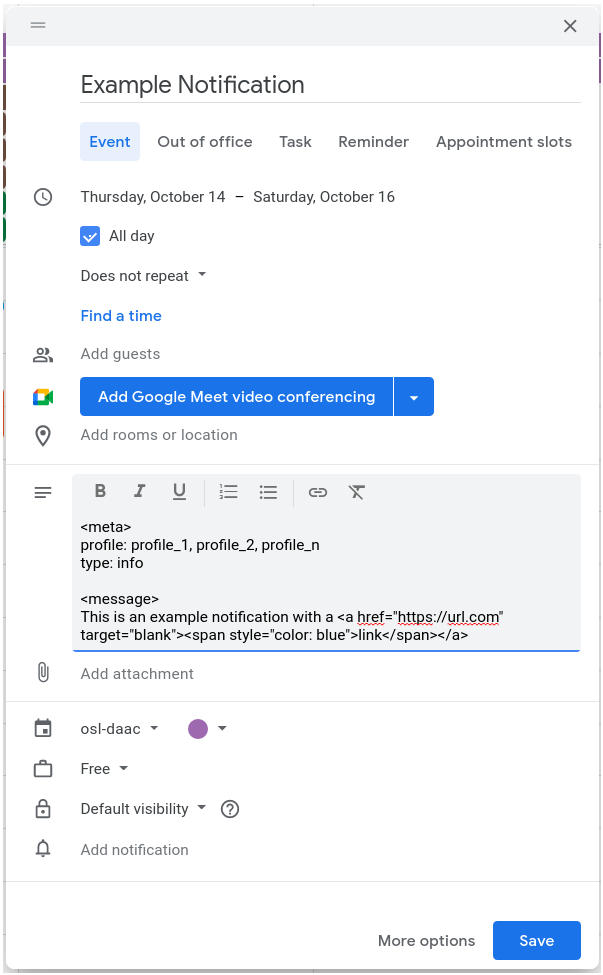
\includegraphics[width=0.7\linewidth]{files/notification-0c08031580ee7d5b2cd20394bd1f7f49.png}
\end{enumerate}
\end{enumerate}
\end{enumerate}
\end{enumerate}
\end{enumerate}

\subsection{Troubleshooting}

\subsubsection{A. Users}

\paragraph{1. OSL Servers Time Out}

\textbf{Problem}: An user's server consistently times out while other users have no difficulty starting a server.

\textbf{Solution}: Respawn the \texttt{hub} pod. Sometimes an internal state within \texttt{hub} gets out of sync with the actual state.

To respawn the \texttt{hub} pod, in a terminal:

\begin{enumerate}
\item \texttt{sk \textless name-of-cluster\textgreater }
\item \texttt{kubectl get pods}
\item \texttt{kubectl delete pod \textless name-of-hub-pod\textgreater }
\end{enumerate}

\subsection{Custom MintPy Conda Build}

\subsubsection{Build latest mintpy and push to custom OpenSARLab conda channel}

Sometimes the latest version of MintPy is desired within a notebook but the official release is not current. These instructions will show how to build MintPy and push to a custom conda channel.

\textit{This assumes that the user has an \href{http://Anaconda.org}{Anaconda.org} account and that this account is attached to a \texttt{OpenSARLab} conda channel. Instructions on how to do this are not provided here.}

A. Create working directory

\begin{verbatim}
mkdir conda -mintpy
cd conda -mintpy
\end{verbatim}

B. Create conda environment

\begin{verbatim}
conda create -n conda -build python=3.10 anaconda -client
conda activate conda -build
\end{verbatim}

C. Clone conda feedstock of mintpy. \href{https://github.com/conda-forge/mintpy-feedstock}{https://github.com/conda-forge/mintpy-feedstock}

\begin{verbatim}
git clone git@github.com:conda -forge/mintpy -feedstock.git
\end{verbatim}

D. Clone mintpy code repo. \href{https://github.com/insarlab/mintpy}{https://github.com/insarlab/mintpy}. Only the latest commit is included to speed up download. Drop the \texttt{--depth 1} to get the whole history.

\begin{verbatim}
git clone - -depth 1 git@github.com:insarlab/MintPy.git
\end{verbatim}

E. Assuming mintpy main is used and is also the latest, we won't make any changes to mintpy

The feedstock is a framework for building. It does not have the source code to build within it. Copy Mintpy source to feedstock recipes.

\begin{verbatim}
cp -r MintPy mintpy -feedstock/recipe/MintPy
\end{verbatim}

F. Make versioning clear and build MintPy from local. The VERSION here is a working example. The actual version is subject to change.

\begin{verbatim}
VERSION=1.3.3.dev.COMMIT_SHORT_HASH
\end{verbatim}

G. Edit \texttt{mintpy-feedstock/recipe/meta.yaml}

\begin{verbatim}
-{% set version = "1.3.2" %}
+{% set version = 1.3.3.dev.COMMIT_SHORT_HASH %}

source:
 -    url: https://github.com/insarlab/{{ name }}/archive/refs/tags/v{{ version }}.tar.gz
 -    sha256: 6c1242dee74f13b96aa4b1f8d50c45ec486397796e4bd4bf3f67849f921bfe7f
+    path: MintPy
\end{verbatim}

H. Build
This may take a while.

\begin{verbatim}
cd mintpy -feedstock
python3.10 build -locally.py
cd ..
\end{verbatim}

I. After a successful build, check for artifacts in \texttt{mintpy-feedstock/build\_artifacts/}

J. Push changes to OpenSARLab conda channel.

\begin{verbatim}
# Login to individual account where you are an owner of OpenSARLab org
anaconda login

# Upload artifacts
anaconda upload - -user opensarlab mintpy -feedstock/build_artifacts/noarch/mintpy -*.tar.bz2
\end{verbatim}

K. Download and check version

\begin{verbatim}
mamba install -c opensarlab -c conda -forge mintpy=VERSION
conda list | grep -i mintpy
\end{verbatim}

L. Cleanup as desired

\begin{verbatim}
cd ../
ls

rm -rf conda -mintpy

conda deactivate
conda env remove -n conda -build
conda env list
\end{verbatim}

\section{Release Notes}

\include{book-release-notes-toc}

\subsubsection{June 2021}

Welcome to the June 2021 OpenSARlab Upgrade!

\subparagraph{Changes:}

\begin{itemize}
\item conda environments \textbf{(BREAKING CHANGE ALERT: please read details below)}
\item nbgitpuller patch
\item installed jupyter-resource-usage
\item profile identifier
\end{itemize}

\paragraph{Conda Environments}

\subparagraph{What is conda and what are conda environments?}

\href{https://docs.conda.io/en/latest/}{Conda} is an open-source package and environment manager. It identifies and attempts to handle dependency related issues when installing multiple software packages. Users create conda environments, in which multiple software packages may be installed. This allows a user to setup a variety of environments, each containing an assortment of software suited to a particular use-case. If a user needs to install software that would conflict with a previously installed package, they can create a new environment in which to install it and avoid the conflict. They can then switch between environments to handle various use-cases.

\subparagraph{How did OpenSARlab use conda previously?}

OpenSARlab previously had conda installed but it was only used as a package manager. Conda was not initialized.

\subparagraph{What problems did this cause?}

\begin{itemize}
\item Not initializing conda made it difficult for users to create and use conda environments effectively
\item All notebooks ran in the same environment, which involved a delicate balance of software installations, making the OpenSARlab docker image very brittle
\item All user accounts had every package installed regardless of individual need, making the OpenSARlab docker image unnecessarily large and slow to build
\item Changes to the conda environment made by users did not persist after server shutdowns
\item Packages such as ISCE, MintPY, TRAIN, and ARIA-Tools were installed in an area to which users lacked access, making updates and development of those packages difficult
\end{itemize}

\subparagraph{What has changed?}

\begin{itemize}
\item All notebooks now run in one of 5 conda environments, each suited different use-cases\begin{itemize}
\item rtc\_analysis
\item insar\_analysis
\item machine\_learning
\item hydrosar
\item Python 3 (the base conda environment containing minimal software)
\end{itemize}


\item Conda environments are stored in /home/jovyan/.local/envs\begin{itemize}
\item this location is on the user volume, so changes persist after server restarts
\end{itemize}


\item New OpenSARlab users are prompted to select the environments they would like pre-built for them when signing up for an account\begin{itemize}
\item unselected environments may always be added later
\end{itemize}


\item Current users must build their own environments using the provided \href{https://github.com/ASFOpenSARlab/opensarlab-envs/blob/main/Create\_OSL\_Conda\_Environments.ipynb}{notebook} and accompanying environment.yml files
\item Python kernels from the appropriate environments have been pre-selected for all notebooks and saved in their metadata\begin{itemize}
\item if the needed environment doesn't yet exist, users will be prompted to change the kernel to one that does
\item Note that an incorrect environment will likely be missing needed software and be incapable of running a notebook for which it was not intended\begin{itemize}
\item Instead, create the needed environment using this \href{https://github.com/ASFOpenSARlab/opensarlab-envs/blob/main/Create\_OSL\_Conda\_Environments.ipynb}{notebook}
\end{itemize}
\end{itemize}


\item Code has been added to each notebook to check that it is running in the correct environment\begin{itemize}
\item Warnings explain how to change to the correct environment if it has been created but the notebook isn't using it
\item Warnings direct users to a \href{https://github.com/ASFOpenSARlab/opensarlab-envs/blob/main/Create\_OSL\_Conda\_Environments.ipynb}{notebook} to create the environment if it does not yet exist
\end{itemize}


\item There is also a minimal environment called ``scratch'' that is intended for user adaptation and experimentation\begin{itemize}
\item This has been added for quick and easy access but users may add as many custom environments as they like
\end{itemize}
\end{itemize}

\subparagraph{What will happen if I don't create any new environments?}

You will encounter environment warnings in the notebooks. You will not have access to the software needed to run the notebooks, which will trigger errors (ModuleNotFoundError).

\subparagraph{I don't want to wait for the notebooks to yell at me and give me environment warnings. How can I create the environments I'd like right now?}

Good choice! Head over to \href{https://github.com/ASFOpenSARlab/opensarlab-envs/blob/main/Create\_OSL\_Conda\_Environments.ipynb}{Create\_OSL\_Conda\_Environments.ipynb} and run the notebook. You will be prompted to select an environment from a list of options. Rerun the notebook for every environment you wish to add.

\paragraph{nbgitpuller Patch}

\subparagraph{What is nbgitpuller?}

\href{https://github.com/jupyterhub/nbgitpuller}{nbgitpuller} performs automatic merging of git repositories in a class-like setting. It handles merging in situations where instructor provided files may be edited both by students and/or the instructor. Its goal is to pull in an instructor's changes while preserving any edits a student has made. Where a conflict exists, it saves the student altered file with a timestamp appended to the filename and pulls in the instructor update.

\subparagraph{What was wrong with nbgitpuller?}

nbgitpuller did not successfully handle all scenarios encountered in OpenSARlab. When it failed, users were locked out of their accounts. They had to login using a purpose-built profile that would skip the nbgitpuller. They could then identify and manually rectify the git state that caused the nbgitpuller to fail.

\subparagraph{How was this issue addressed?}

We have populated user accounts with an altered version of nbgitpuller/pull.py

\begin{itemize}
\item The nbgitpuller will no longer attempt to checkout files that have been removed from a remote branch
\item If the user has changed to a branch other than main in the \href{https://github.com/ASFOpenSARlab}{opensarlab-notebooks} git repository, the merge will be aborted
\item Users can still merge other branches from the command line
\end{itemize}

\paragraph{Installed jupyter-resource-usage}

\subparagraph{What is jupyter-resource-usage?}

\href{https://github.com/jupyter-server/jupyter-resource-usage}{jupyter-resource-usage} is an extension that displays how much memory a notebook server is using. The information is displayed at the top-right of every running Jupyter Notebook. It indicates the total memory used by all running notebooks, kernels, terminals, etc.

\paragraph{Added profile identifier}

The name of the current profile now appears to the left of the ``Logout'' button on the home page.

\subsubsection{October 2021}

Welcome to the October 2021 OpenSARlab Upgrade!

\subparagraph{Changes:}

\begin{itemize}
\item Pull in the \href{https://github.com/uafgeoteach/GEOS657\_MRS}{GEOS657\_MRS repository}
\item OpenSARlab documentation changes
\item Add OpenSARlab documentation link to the top of every page
\item Add current profile name to the top of every page
\end{itemize}

\paragraph{Conda Environments}

\subparagraph{Pull in The \href{https://github.com/uafgeoteach/GEOS657\_MRS}{GEOS657\_MRS Repository}}

\begin{itemize}
\item The GEOS\_657\_Labs directory has been removed from the \href{https://github.com/ASFOpenSARlab/opensarlab-notebooks}{opnesarlab-notebooks repository} and moved into its own repository, \href{https://github.com/uafgeoteach/GEOS657\_MRS}{uafgeoteach/GEOS657\_MRS}
\item The notebooks in the \texttt{/home/jovyan/notebooks/ASF/GEOS\_657\_Labs} directory can now be found in the \texttt{/home/jovyan/GEOS\_657\_Labs} directory.
\item If you made any changes to the notebooks in their original location, you may still see them there, but necessary scripts may be missing and you should start working out of the new location.
\end{itemize}

\subparagraph{OpenSARlab documentation changes}

\begin{itemize}
\item OpenSARlab documentation is no longer being stored in \texttt{/home/jovyan/opensarlab\_docs} in Jupyter Notebook form.
\item There is now a link to the \href{https://opensarlab-docs.asf.alaska.edu/}{OpenSARlab-docs website} at the top of every page in OpenSARlab.
\end{itemize}

\subparagraph{Add current profile name to the top of every page}

\begin{itemize}
\item Different OpenSARlab profiles allow for varying resource allotments.
\item The current profile name now appears at the top of every OpenSARlab page to serve as a reminder to the user of which profile they are running in.
\end{itemize}

\subsubsection{February 2022}

Welcome to the February 2022 OpenSARLab Update!

\subparagraph{Changes:}

\begin{itemize}
\item Ubuntu 20.04.3 LTS
\item JupyterLab
\item Matplotlib widget
\item Url-widget
\item New memory monitor location
\item Notebook Debugger
\item Mamba
\item Mamba Gator
\item Spellchecker
\item Custom extensions
\item Recommended Jupyter Notebook changes related to update
\end{itemize}

\paragraph{Ubuntu 20.04.3 LTS}

\begin{itemize}
\item JupyterHub is now running on Ubuntu 20.04.3 LTS, updated from Ubuntu 18.04
\end{itemize}

\paragraph{JupyterLab}

\begin{itemize}
\item There are now JupyterLab profiles available alongside the Classic Jupyter Notebook profiles. JupyterLab comes with many more features than Classic Jupyter Notebook (see the \href{https://jupyterlab.readthedocs.io/en/stable/user/interface.html}{JupyterLab Docs}) for more information.
\item Classic Jupyter Notebook profiles will remain active for 1 month before being deprecated on March 7th.
\end{itemize}

\paragraph{Matplotlib widget}

\begin{itemize}
\item \texttt{matplotlib notebook} has been replaced with \texttt{matplotlib widget} for interactive matplotlib plots.\begin{itemize}
\item \texttt{matplotlib notebook} will not work in JupyterLab, whereas \texttt{matplotlib widget} works in both JupyterLab and Classic Jupyter Notebook.
\end{itemize}
\end{itemize}

\paragraph{Url-widget}

\begin{itemize}
\item The \texttt{url-widget} package is now installed, allowing notebook Python kernels access to the current notebook's URL.\begin{itemize}
\item This is useful for dynamically creating links to files and notebooks in OpenSARlab, and it is used in the kernel checking code at the beginning of ASF provided notebooks.
\end{itemize}
\end{itemize}

\paragraph{New Memory Monitor Location}

\begin{itemize}
\item JupyterLab comes with a built-in memory monitor, replacing the jupyter-resource-usage extension.\begin{itemize}
\item The new memory monitor can be found in the status bar at the bottom of the JupyterLab screen.
\end{itemize}
\end{itemize}

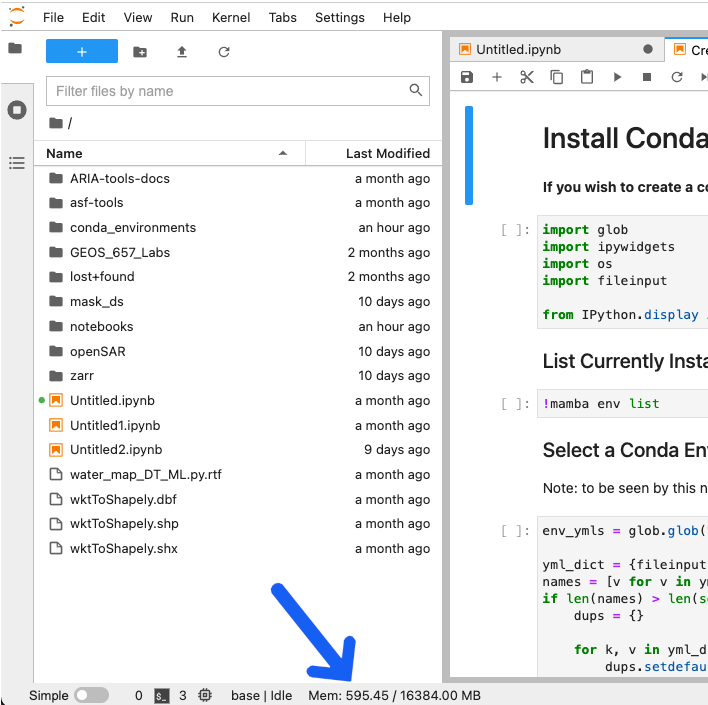
\includegraphics[width=0.7\linewidth]{files/memory_monitor-b336a1d9ea9c428bf307532d53b564ff.png}

\paragraph{Notebook Debugger}

\begin{itemize}
\item JupyterLab comes with a built-in notebook debugger.\begin{itemize}
\item \href{https://jupyterlab.readthedocs.io/en/stable/user/debugger.html}{JupyterLab Debugger Docs}
\end{itemize}
\end{itemize}

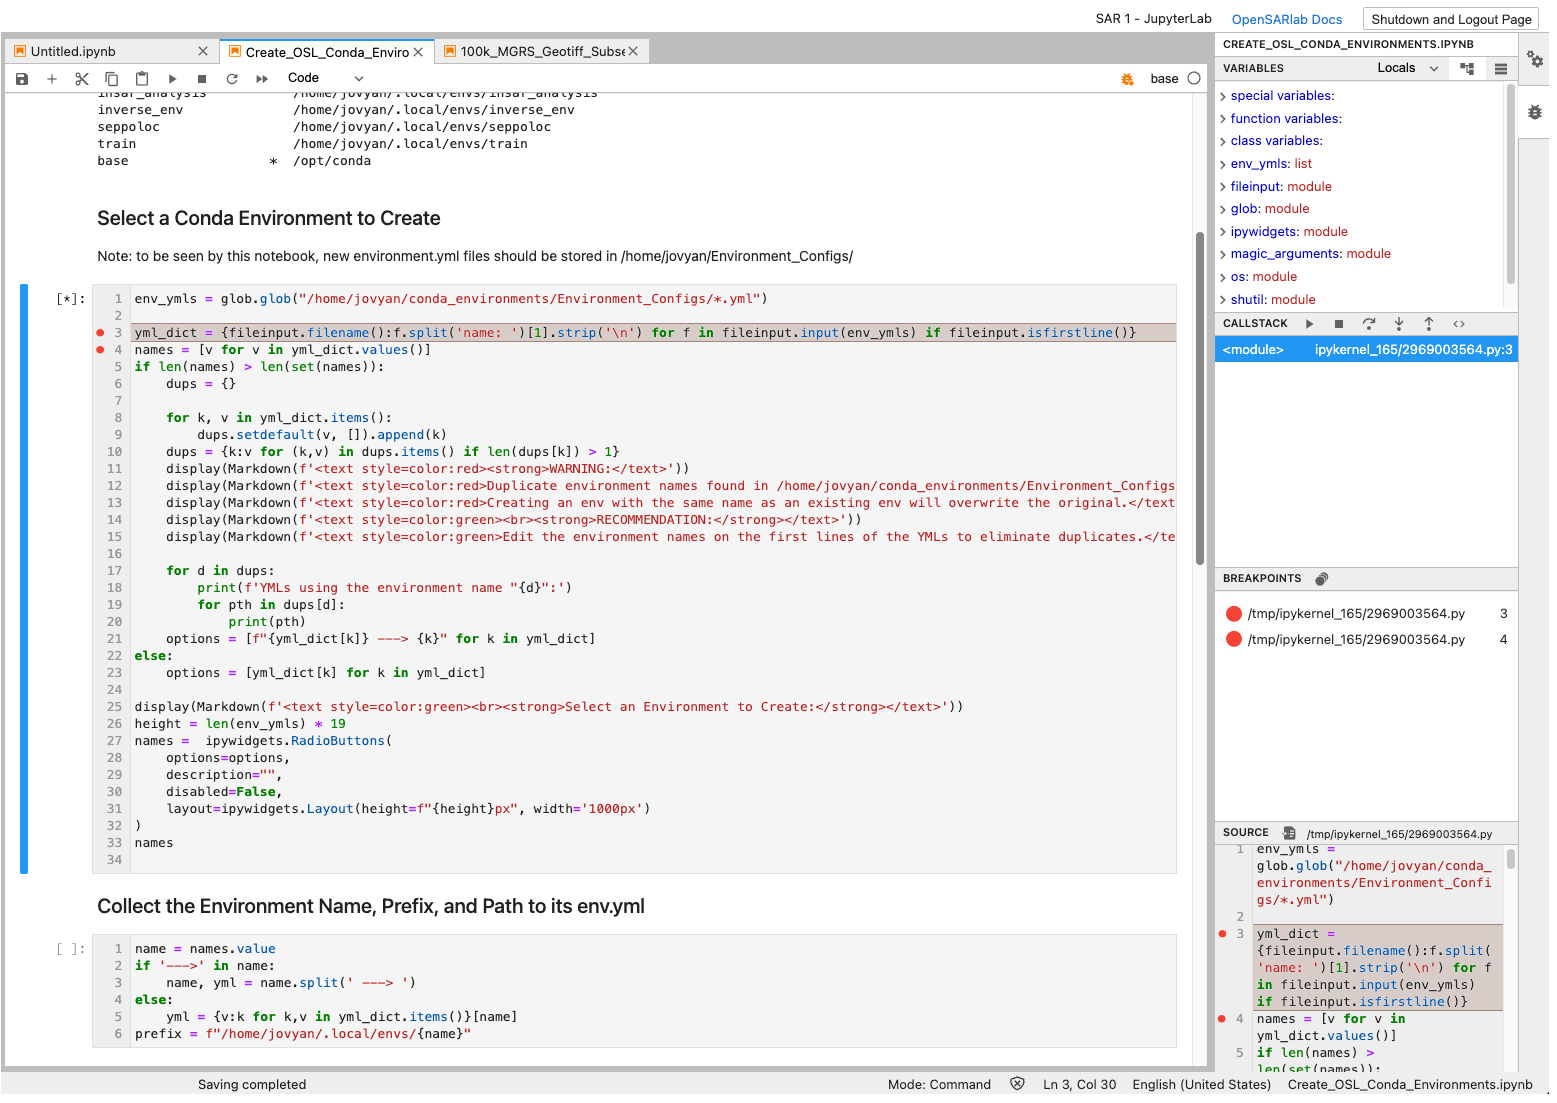
\includegraphics[width=0.7\linewidth]{files/debugger-c772ddfa3cdf2824afc44735f30281be.png}

\paragraph{Mamba}

\begin{itemize}
\item The \href{https://github.com/mamba-org/mamba}{mamba package manager} is now available in OpenSARlab.\begin{itemize}
\item Mamba is a multi-threaded ``reimplementation of the conda package manager in C++.''\begin{itemize}
\item It creates environments much more quickly than conda.
\end{itemize}
\end{itemize}


\item The \href{https://github.com/ASFOpenSARlab/opensarlab-envs}{opensarlab-envs repo} has been updated to use mamba.
\end{itemize}

\paragraph{Mamba Gator is installed}

\begin{itemize}
\item \href{https://github.com/mamba-org/gator}{mamba gator} provides a GUI for managing conda/mamba environments that is accessible in JupyterLab.\begin{itemize}
\item Access mamba gator by selecting the  \texttt{Conda Packages Manager} from the \texttt{Settings} menu.
\end{itemize}
\end{itemize}

\paragraph{Spellchecker}

\begin{itemize}
\item The \href{https://github.com/jupyterlab-contrib/spellchecker}{spellchecker extension} is installed.\begin{itemize}
\item It checks spelling in markdown cells.
\item The language may be changed in the status bar at the bottom of the screen.
\end{itemize}
\end{itemize}

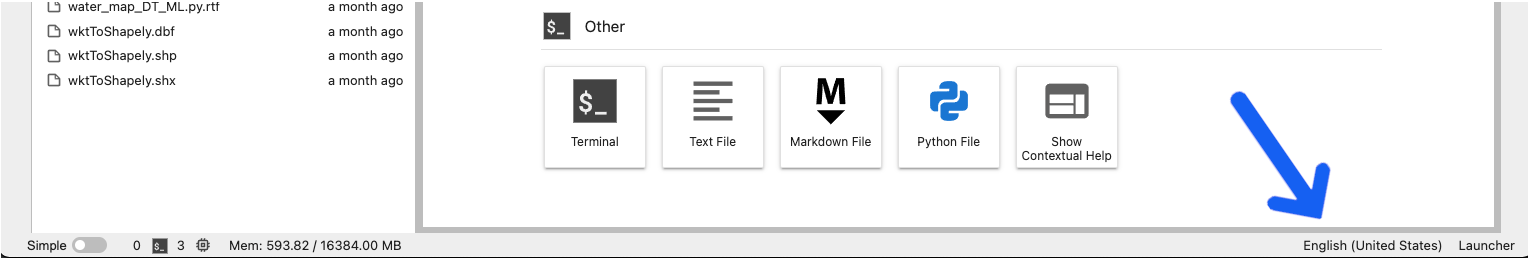
\includegraphics[width=0.7\linewidth]{files/language-7731ca45e6f15149a0b8842980445c71.png}

\paragraph{Custom Extensions}

\begin{itemize}
\item We have added some custom JupyterLab extensions to duplicate custom features previously added in OpenSARlab for Jupyter Notebooks.\begin{itemize}
\item \href{https://pypi.org/project/opensarlab-profile-label/}{opensarlab-profile-label} provides the name of the current OpenSARlab profile in the topbar.
\item \href{https://pypi.org/project/opensarlab-doc-link/}{opensarlab-doc-link} provides a link to the \href{https://opensarlab-docs.asf.alaska.edu/}{OpenSARlab documentation} in the topbar.
\item \href{https://pypi.org/project/opensarlab-controlbtn/}{opensarlab-controlbtn} provides a \texttt{Shutdown and Logout Page} button in the topbar.
\item \href{https://pypi.org/project/opensarlab-notifications/}{opensarlab-notifications} provides similar functionality to the popup notifications used in the OpenSARlab Classic Jupyter Notebook profiles.
\end{itemize}
\end{itemize}

\paragraph{Recommended Jupyter Notebook Changes}

The following bullet points cover code changes you may need to make to your notebooks for them to work in JupyterLab

\textit{note: These changes are backwards compatible and updated notebooks will still run in Jupyter Notebook.}

\textit{note: All \href{https://github.com/ASFOpenSARlab/opensarlab-notebooks}{ASF notebooks} have already been updated.}

\begin{itemize}
\item The javascript variable \texttt{Jupyter.notebook.kernel} does not exist in JupyterLab.\begin{itemize}
\item If you need a Python variable containing a notebook's current Python kernel, run:\begin{itemize}
\item \texttt{env = !echo \$CONDA\_PREFIX}
\end{itemize}
\end{itemize}


\item The javascript variable \texttt{window.location} does not exist in JupyterLab\begin{itemize}
\item If you need the current url of your Jupyter workspace, install the \texttt{url-widget} package in your conda environment and use it to retrieve the url:
\end{itemize}
\end{itemize}

\begin{verbatim}
# In one cell
import url_widget as url_w
notebook_url = url_w.URLWidget()
display(notebook_url)
\end{verbatim}

\begin{verbatim}
# In a following cell
notebook_url = notebook_url.value
\end{verbatim}

\begin{itemize}
\item \texttt{\%matplotlib notebook} does not work for interactive plotting in JupyterLab\begin{itemize}
\item Instead, use: \texttt{\%matplotlib widget}
\end{itemize}


\item \texttt{asf\_notebook.py} is deprecated and has been replaced with \texttt{opensarlab-lib}: \href{https://github.com/ASFOpenSARlab/opensarlab-lib}{https://github.com/ASFOpenSARlab/opensarlab-lib}\begin{itemize}
\item \texttt{asf\_notebook.py} still works (with deprecation warnings) but it is not being maintained.
\item Install \texttt{opensarlab-lib} with one of the following commands:\begin{itemize}
\item \texttt{python -m pip install opensarlab-lib}
\item \texttt{conda install -n \textless environment\_name\textgreater  -c conda-forge opensarlab-lib}
\end{itemize}


\item Alternatively, you may add \texttt{environment.yml} as a dependency and use it instead.
\end{itemize}
\end{itemize}

\subsubsection{February 2023}

Welcome to the February 2023 OpenScienceLab Update!

\subparagraph{Changes:}

\begin{itemize}
\item OpenScienceLab
\item Single~Sign~On
\item Automatic~Authentication
\item User~Access
\item IP~Filter
\item User~Request
\item Multi~Download
\item Kernel~Usage
\item Recommended~Jupyter~Notebook~Changes
\end{itemize}


\bigskip
\centerline{\rule{13cm}{0.4pt}}
\bigskip

\paragraph{\textbf{OpenScienceLab}}\label{opensciencelab}

\begin{itemize}
\item OpenSARLab is now a part of OpenScienceLab with significant changes. Users can access different courses from a single page.
\end{itemize}

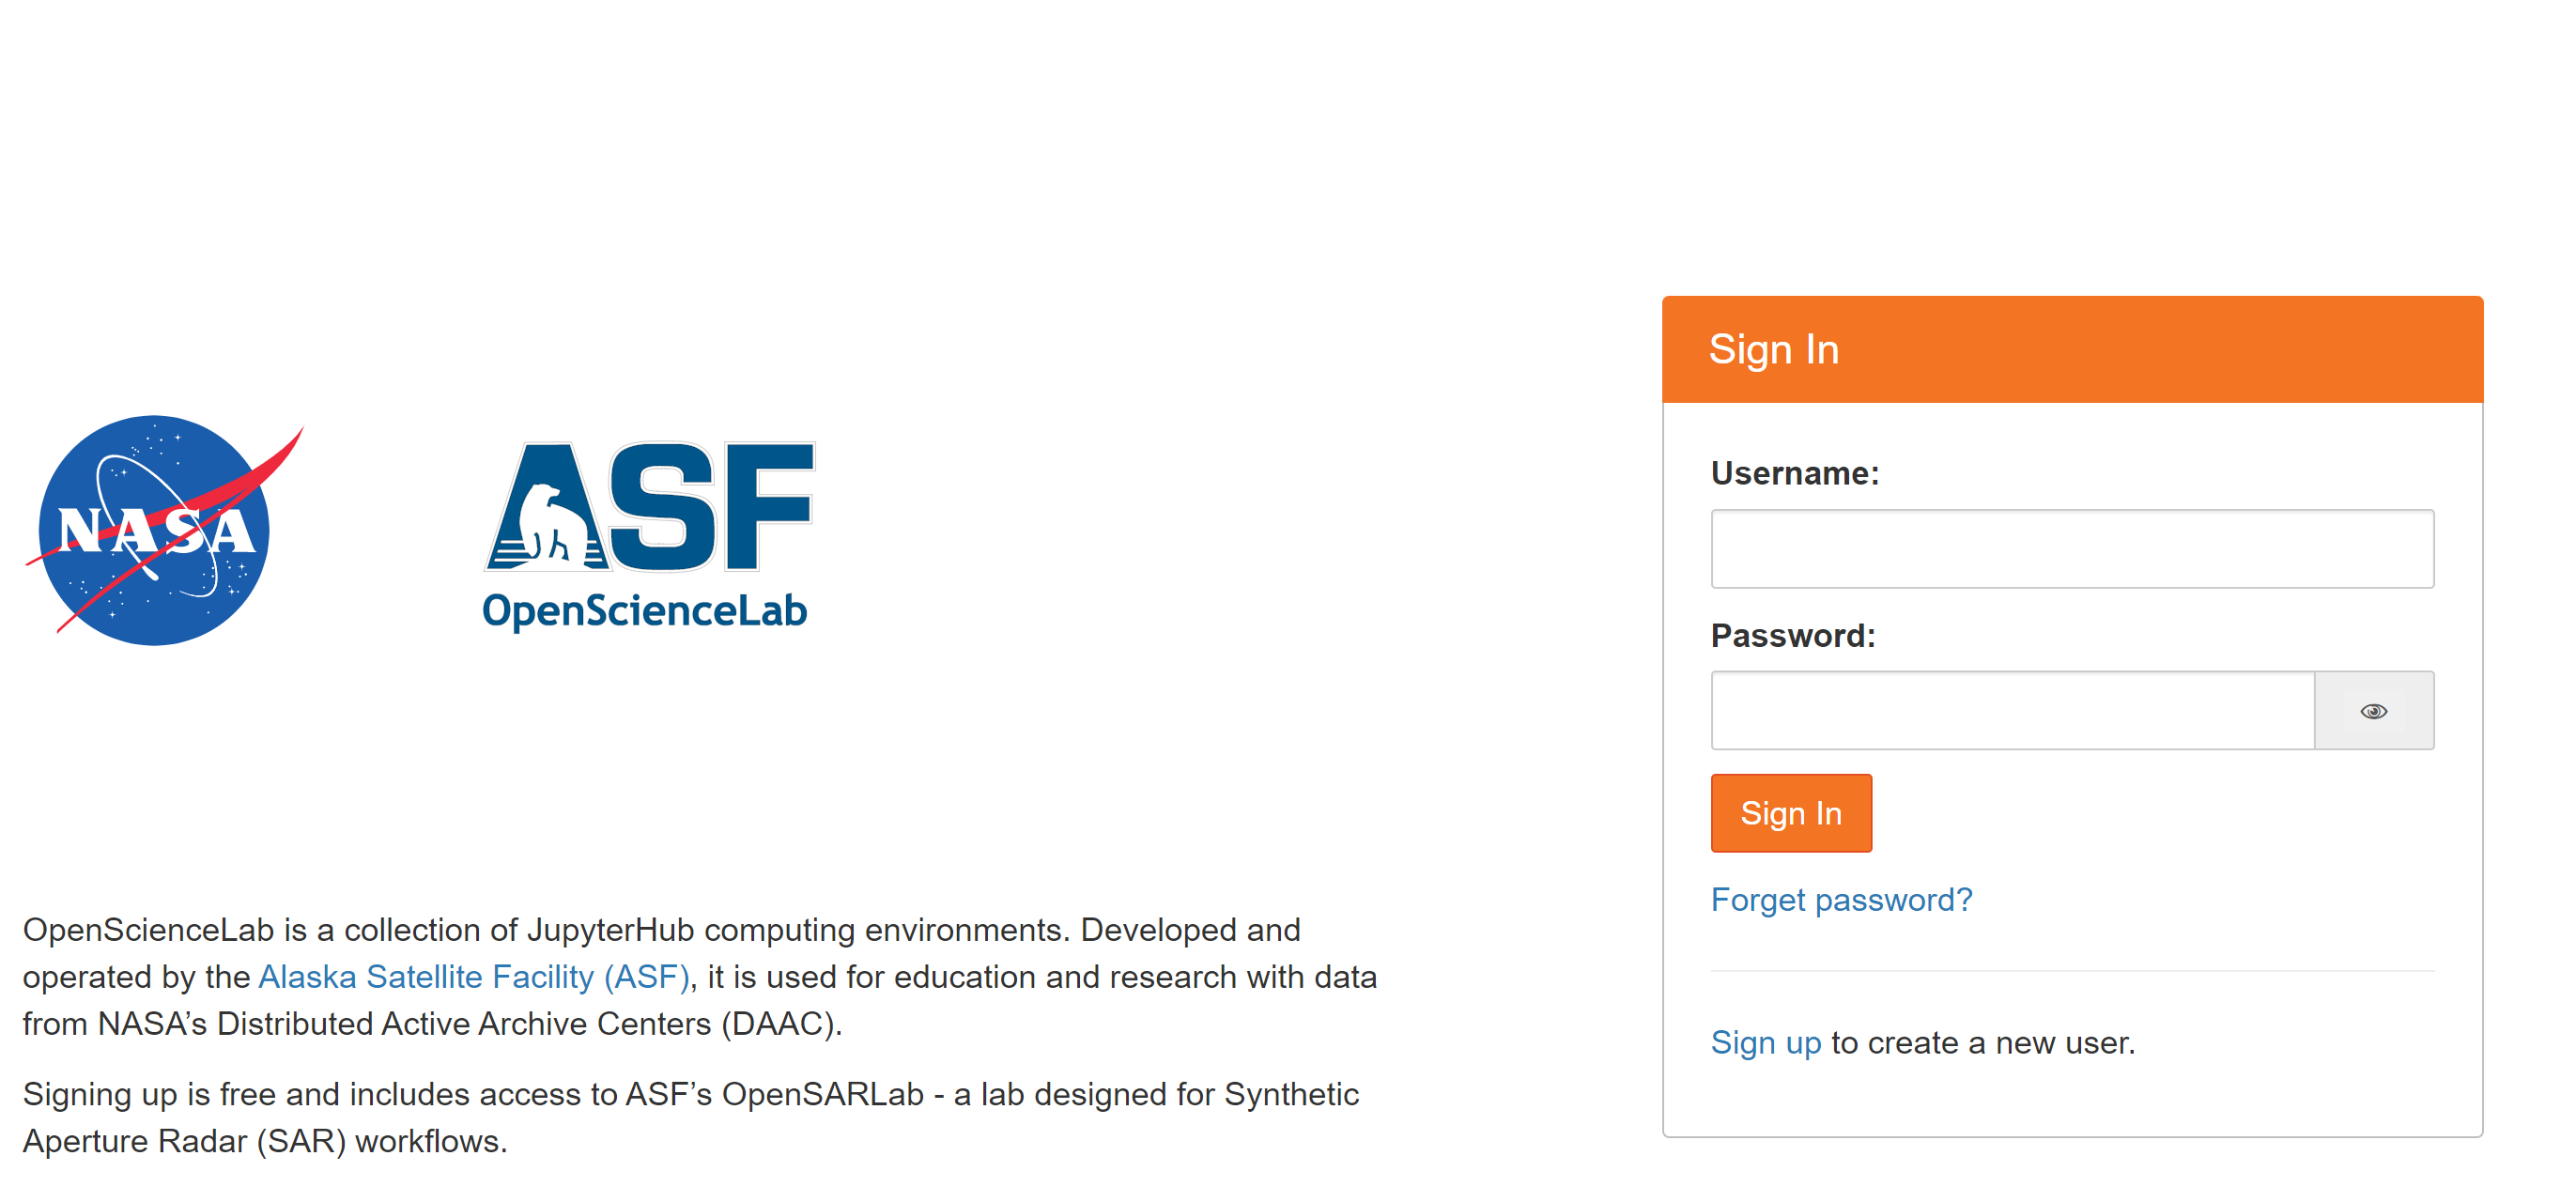
\includegraphics[width=0.7\linewidth]{files/opensciencelab-8e85c9cc58445dc01847745b03f7ec57.PNG}

\paragraph{\textbf{Single Sign On}}\label{single-sign-on}

\begin{itemize}
\item New single sign-on (SSO) to simplify the logging-in process. SSO eliminates the burden of the sign-on process by listing all accounts on a single web page with additional layers of security.
\end{itemize}

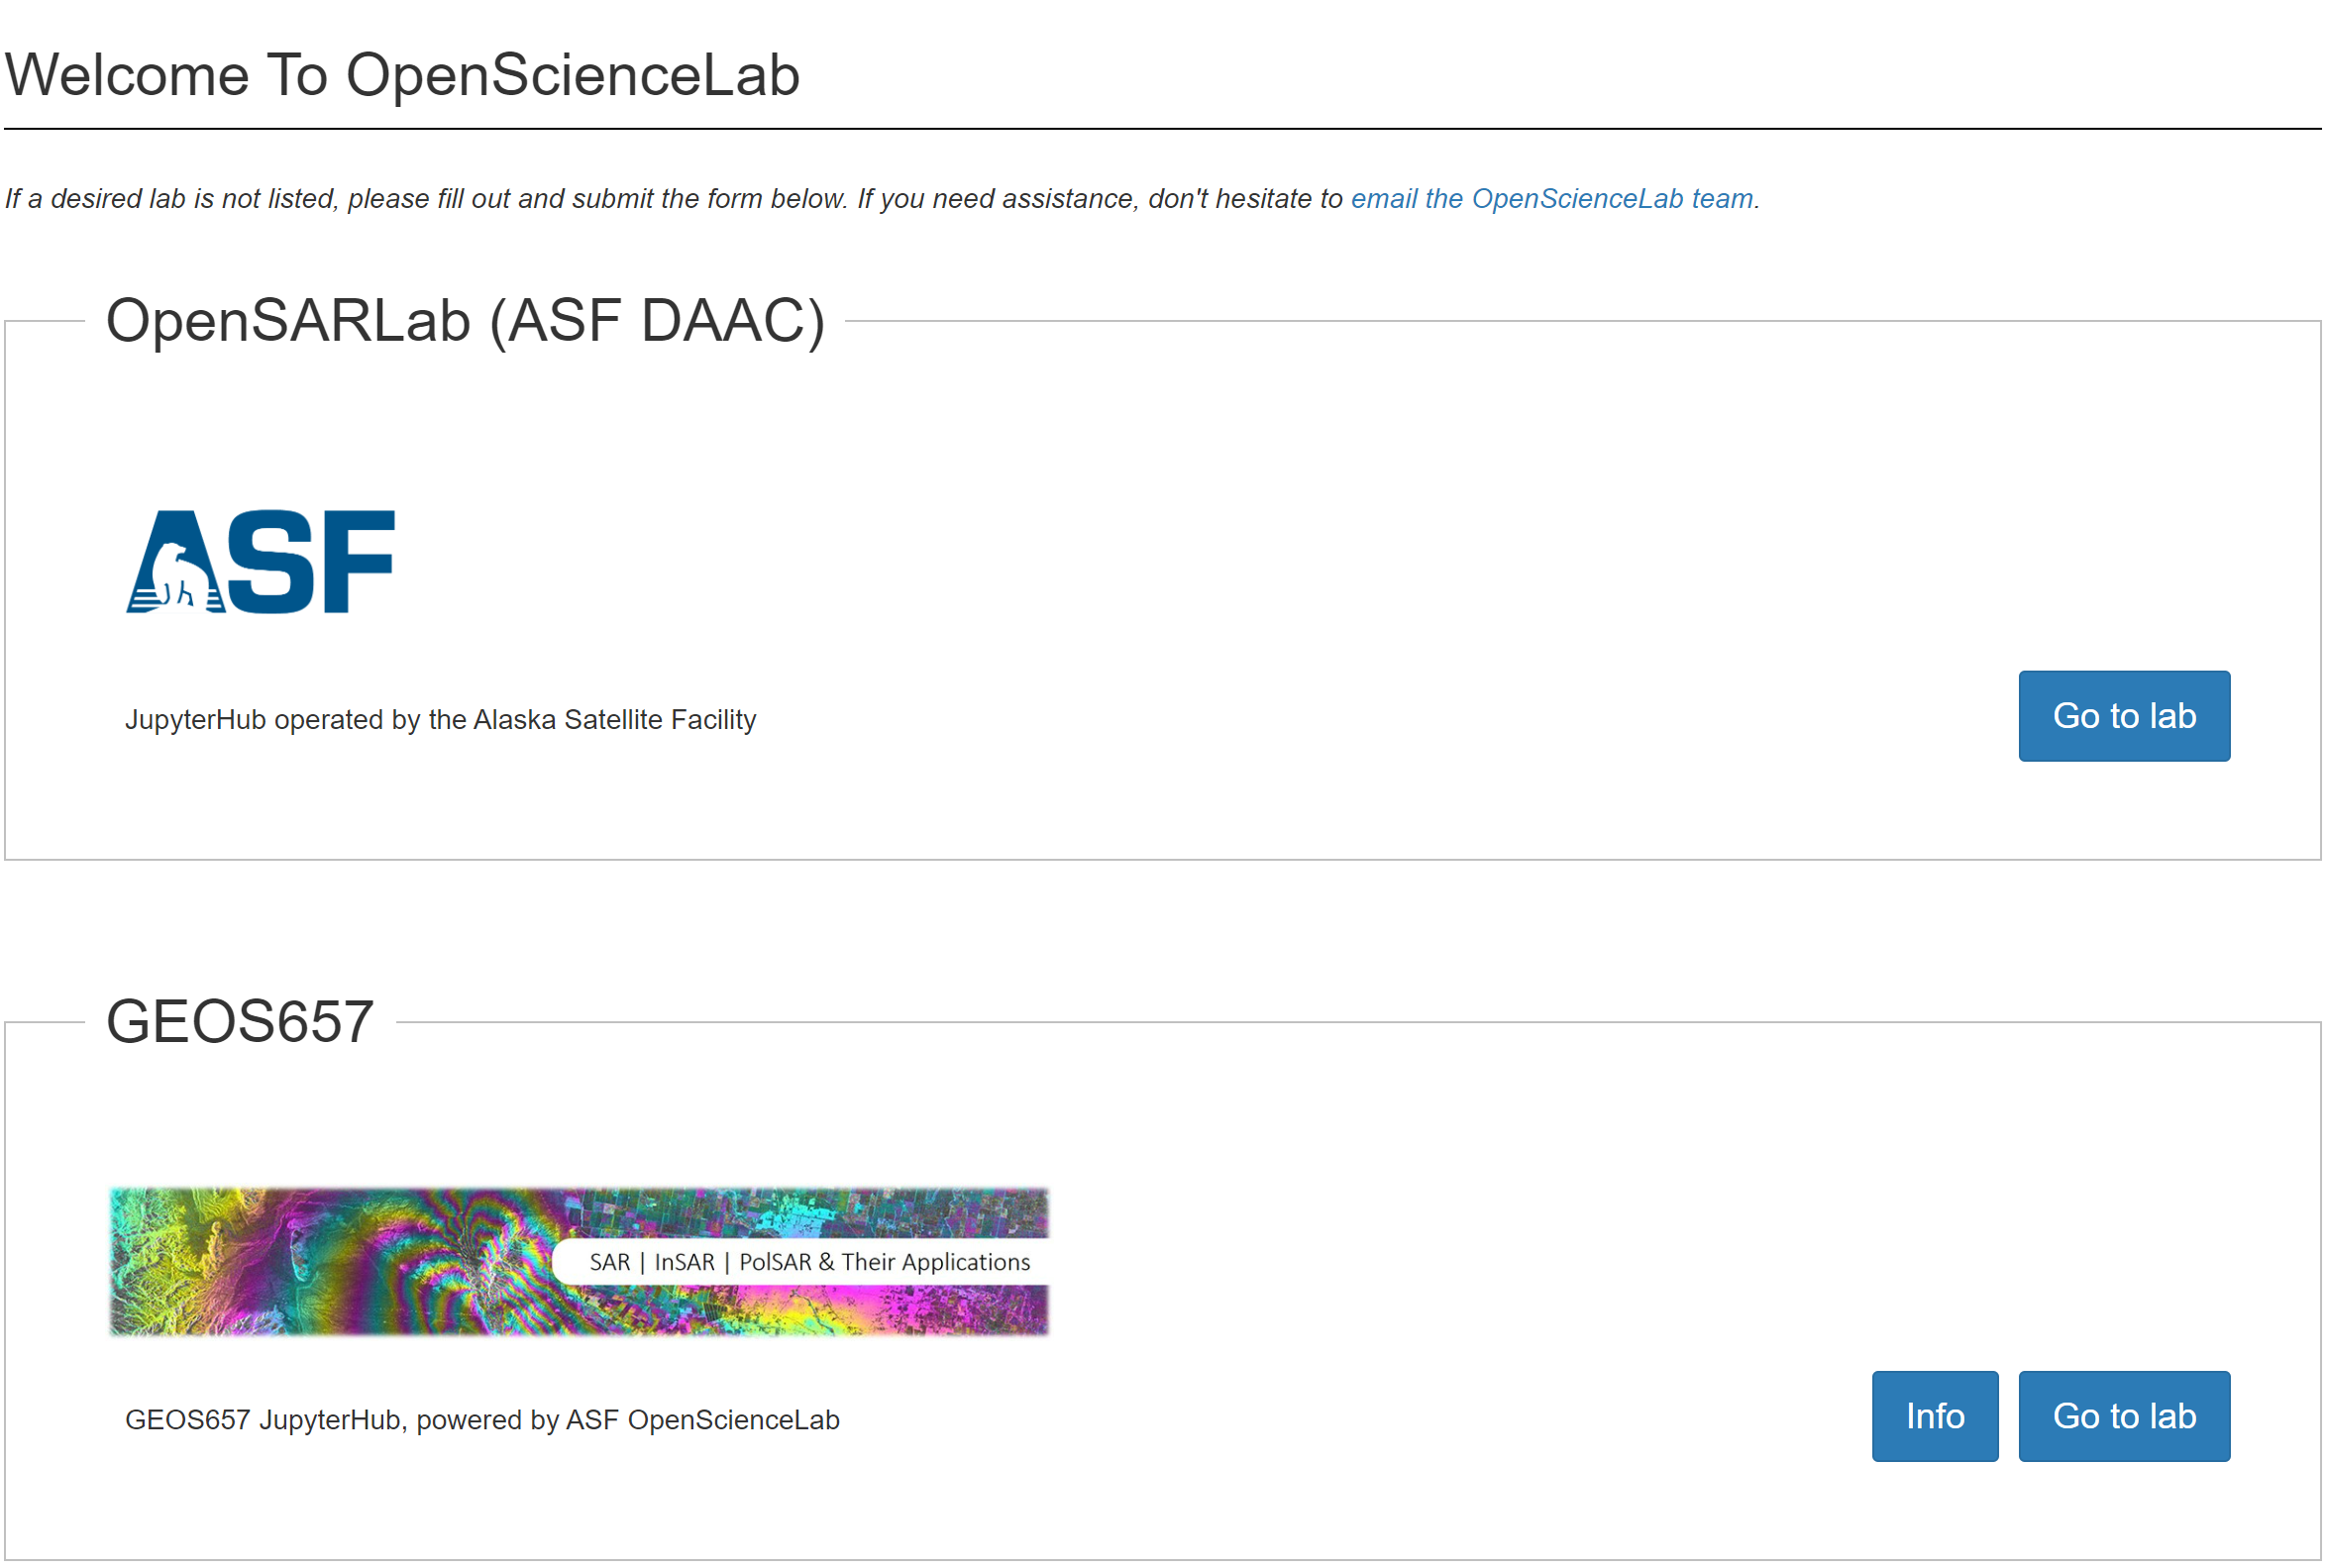
\includegraphics[width=0.7\linewidth]{files/single_sign_on-89eb0d255f0daa91c661c0a2359a6916.PNG}

\paragraph{\textbf{Automatic Authentication}}\label{automatic-authentication}

\begin{itemize}
\item Users who sign up to the OpenScienceLab no longer need admins to activate their accounts.
\end{itemize}

\paragraph{\textbf{User Access}}\label{user-access}

\begin{itemize}
\item Admins can easily give users access to different profiles from a single page. Admins can toggle access lists based on various deployments.
\end{itemize}

\paragraph{\textbf{IP Filter}}\label{ip-filter}

\begin{itemize}
\item OpenScienceLab will prevent users in one of NASA's \href{https://www.nasa.gov/sites/default/files/atoms/files/designated\_country\_list\_6.10.2022.pdf}{designated countries list} from creating an account so that we are compliant with NASA's security protocol.
\end{itemize}

\paragraph{\textbf{User Request}}\label{user-resquest}

\begin{itemize}
\item Users can send a request to the OpenScienceLab team from the portal.
\end{itemize}

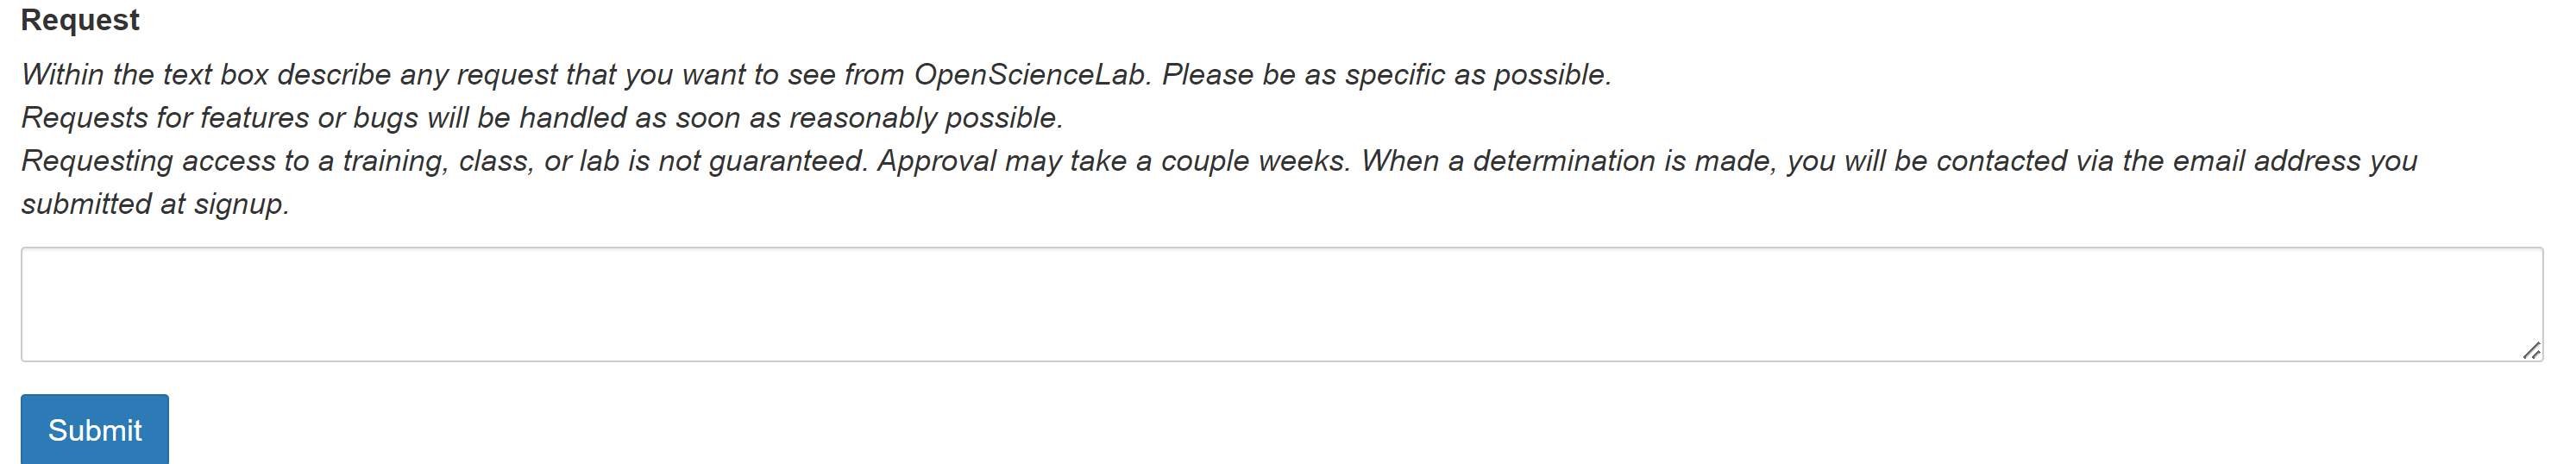
\includegraphics[width=0.7\linewidth]{files/user_request-b4d8f393b11dea7c2cbf0b3baf130dba.PNG}

\paragraph{\textbf{Multi Download}}\label{multi-download}

\begin{itemize}
\item Users can download multiple files at once through OpenScienceLab.
\item \textbf{NB}: Downloading multiple directories requires users to compress the directories beforehand.
\end{itemize}

\includegraphics[width=0.7\linewidth]{files/multi_download-5ee606c2f5273c98a62c6238687f7413.gif}

\paragraph{\textbf{Kernel Usage}}\label{kernel-usage}

\begin{itemize}
\item The latest update of JupyterLab has a built-in kernel monitor that tracks detailed resource usage, such as:\begin{itemize}
\item Kernel Host
\item Memory consumption and availability
\item CPU usage
\end{itemize}
\end{itemize}

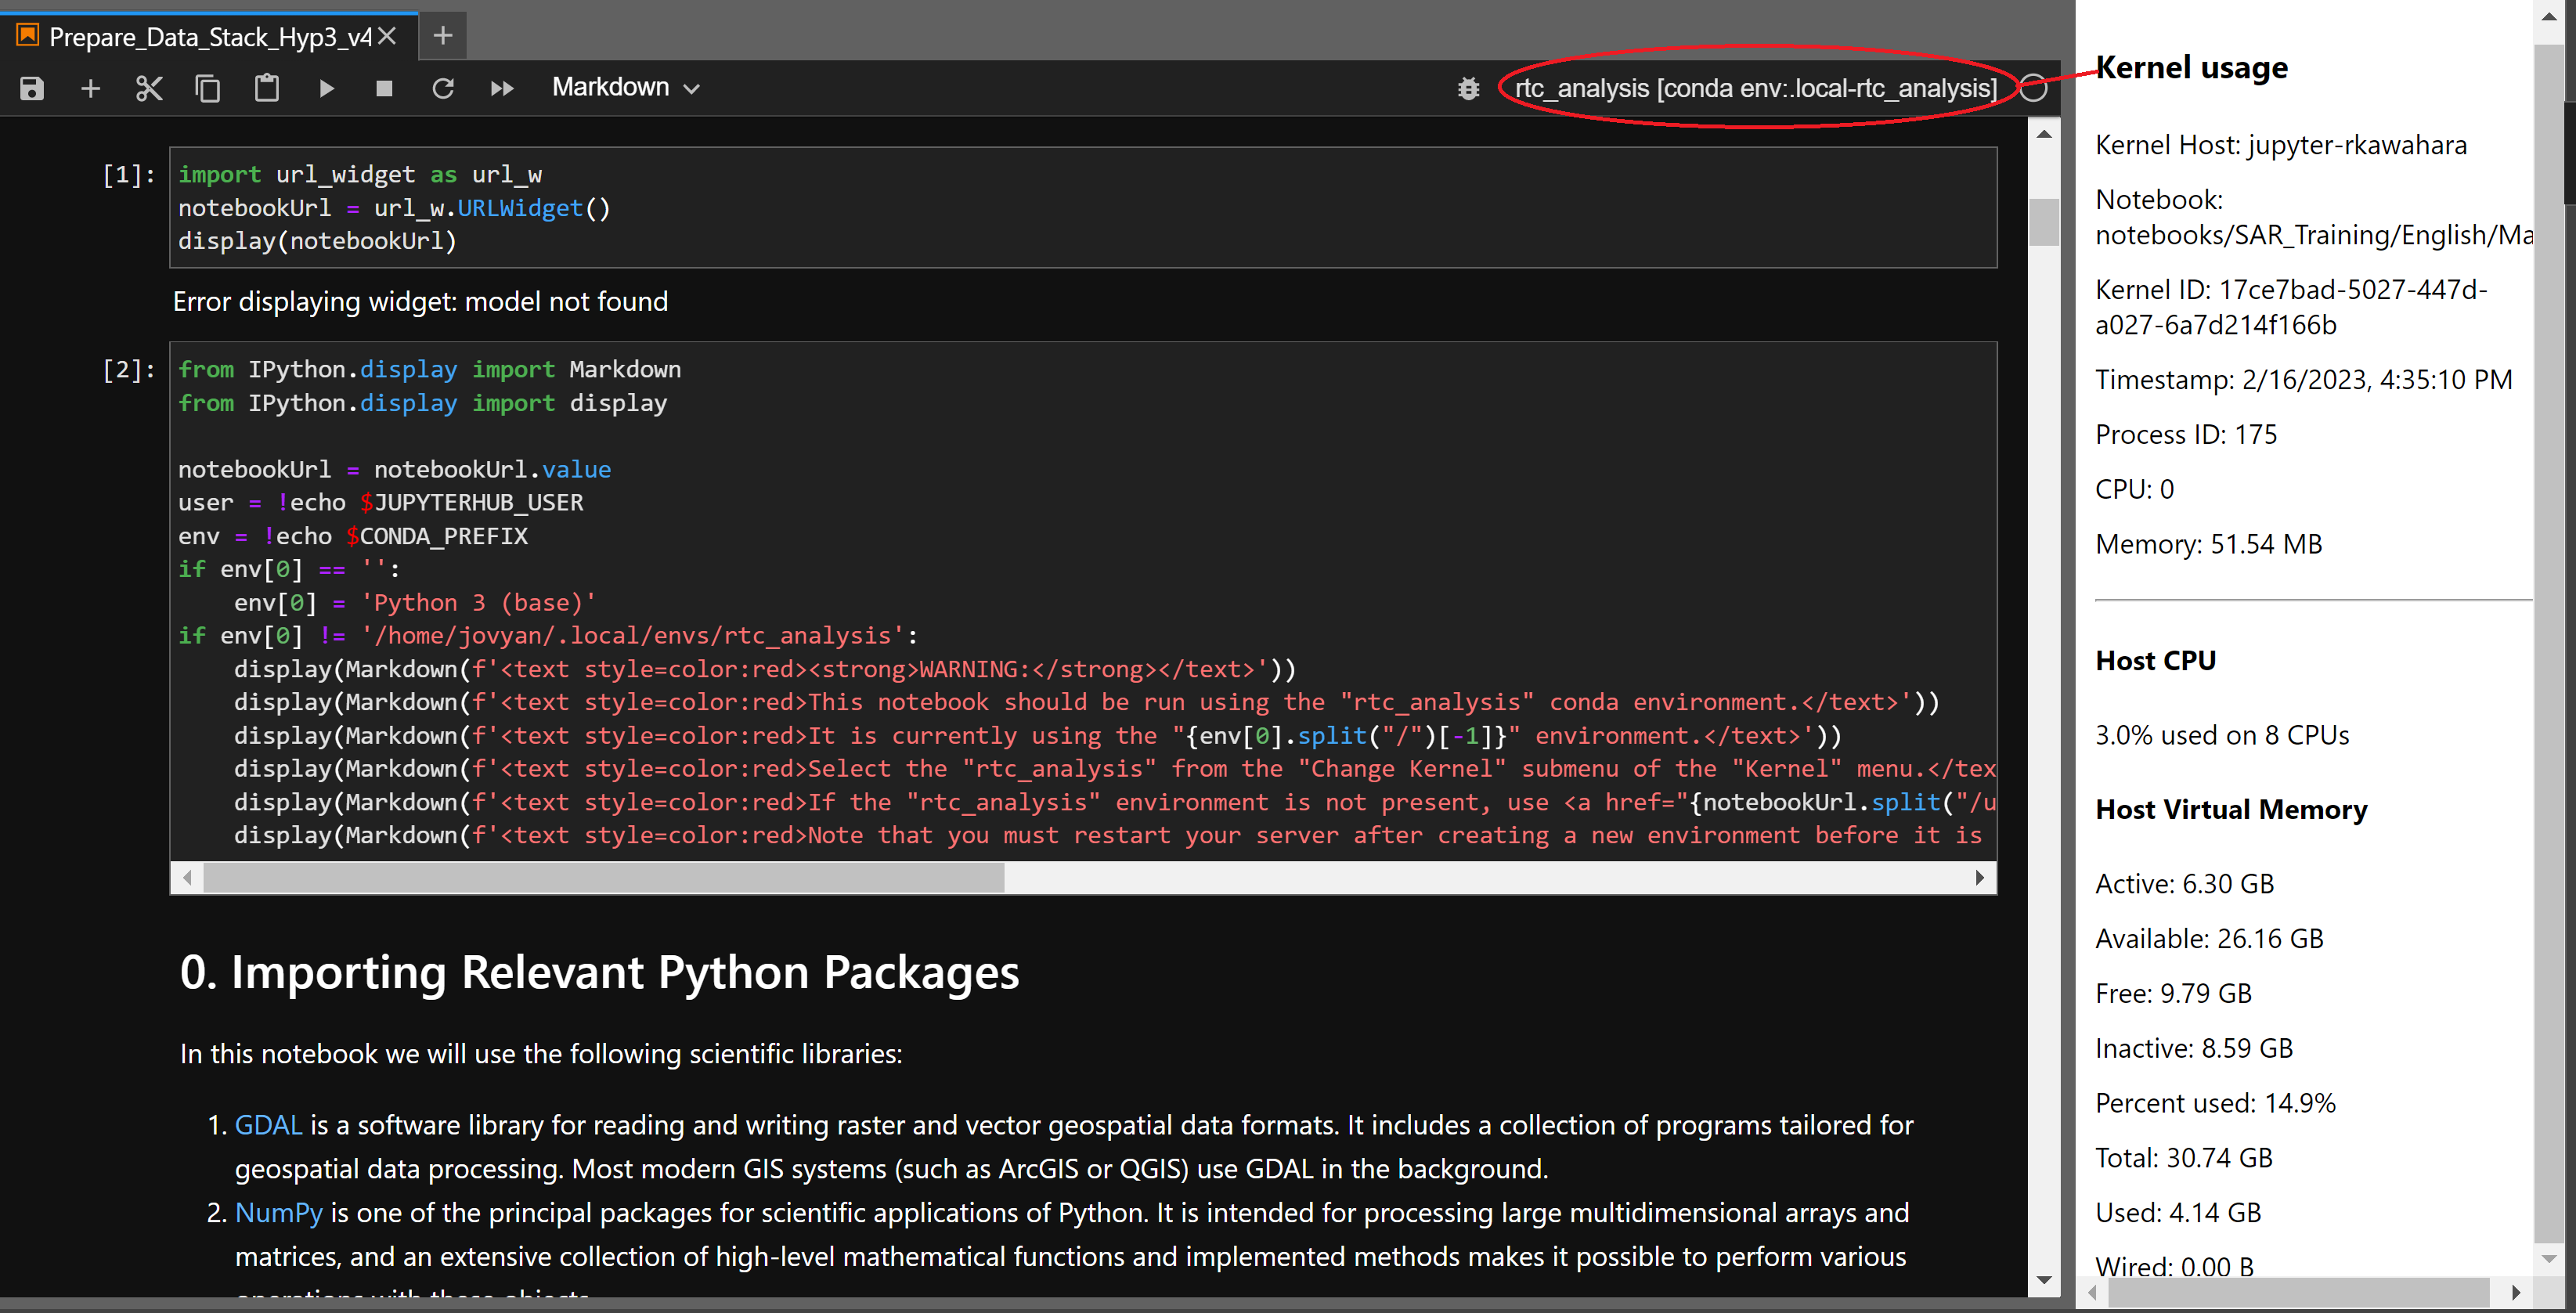
\includegraphics[width=0.7\linewidth]{files/kernel_usage-3999565cdea65e09da8c3bdf1ec55131.PNG}

\paragraph{\textbf{Recommended Jupyter Notebook Changes}}\label{recommended-jupyter-notebook-changes}

The following bullet points cover code changes you may need to make to your notebooks for them to work in JupyterLab:

\begin{itemize}
\item MintPy Update:

Due to the recent MintPy update, import syntax for version 1.4.1+ differs from previous versions. As a result, some notebooks may be incompatible with the latest version of MintPy. Below are examples of how to import MintPy depending on which versions you have:

\begin{verbatim}
# version 1.4.0 and below:
import mintpy.view as view
import mintpy.tsview as tsview
.
.
.

# version 1.4.1+
from mintpy.cli import view, tsview, ...
\end{verbatim}
\end{itemize}

For additional backward compatibility changes, please refer to the previous release notes.

\subsubsection{February 2024}

Welcome to the February 2024 OpenScienceLab Update!

\subparagraph{Changes:}

\begin{itemize}
\item Multi-Factor~Authentication
\end{itemize}


\bigskip
\centerline{\rule{13cm}{0.4pt}}
\bigskip

\paragraph{\textbf{Multi-Factor Authentication}}\label{multi-factor-authentication}

\begin{itemize}
\item OpenScienceLab now requires users to set up Multi-Factor Authentication (MFA)
to access OpenScienceLab resources. Directions on how to do so, as well as
troubleshooting recommendations, can be found on the new
\href{/mfa}{MFA documentation page}
\end{itemize}

\subsubsection{December 2024}

Welcome to the December 2024 OpenScienceLab Update!

\paragraph{Changes:}

Documentation updated to reflect current code for container, cluster, and portal.





\end{document}
